% ----------------------------------------
% Preamble
% ----------------------------------------
% ------- To set document layout -------
% ----------------------------------------
% Preamble: To set document layout
% ----------------------------------------
% ------- To define document class -------
\documentclass[article, crop=false]{standalone}


% ------- To set page size and margins -------
\usepackage[
    letterpaper,
    centering,
    includehead, includefoot,
    top = 1.5cm,
    headheight = 1.0cm, headsep = 1.0cm,
    footskip = 1.0cm,
    left = 2.0cm, right = 2.5cm
]{geometry}


% ------- To set header and footer styles -------
\usepackage{fancyhdr}
\usepackage{lastpage}
\pagestyle{fancy}
\renewcommand{\headrulewidth}{0pt}
\fancyhf{}
\lhead{
    \textbf{\small{\underline{
        SMUD Greenergy Program: Descriptive Analysis
    } \\
    \vspace{0.1cm}
    \emph{Jinmahn Jo} (ID\#: 915528897)}
    }
}
\rfoot{
    \footnotesize{Page  \thepage \hspace{1pt} of \pageref{LastPage}}
}




% ------- To load package(s) required -------
% ----------------------------------------
% Preamble: To load package(s) required
% ----------------------------------------
% ------- To load package(s) required -------
% 1. General
\usepackage[utf8]{inputenc}

% 2. To insert mathematical equations
\usepackage{amsmath, amssymb, amsthm}

% 3. To embed image files
\usepackage{graphicx}
\usepackage{caption, subcaption}

% 4. To embed tables
\usepackage{longtable}
\usepackage{xtab, ltablex}
\usepackage{boldline, rotating, adjustbox}
\usepackage{makecell}

% 4.1. Tables from "fixest" library
\usepackage{booktabs}
\usepackage{threeparttable}
% % 4.2. Tables from "huxtable" library
% \usepackage{array}
% \usepackage{caption}
% \usepackage{graphicx}
% \usepackage{siunitx}
% \usepackage{ulem}
% \usepackage{colortbl}
% \usepackage{multirow}
% \usepackage{hhline}
% \usepackage{calc}
% \usepackage{tabularx}
% \usepackage{threeparttable}
% \usepackage{wrapfig}
% \usepackage{adjustbox}
% \usepackage{hyperref}

% 5. To generate figures
\usepackage{tikz}
\usetikzlibrary{intersections, through, calc, decorations.pathreplacing}

% 6. To change page mode
\usepackage{lscape}




% ------- To define new commands -------
% ----------------------------------------
% Preamble: To define new commands
% ----------------------------------------
% ------- To define new commands -------
% 1. For Mathematical Equations
\renewcommand{\vec}[1]{\mathbf{#1}}
\let \boldhat \hat
\renewcommand{\hat}[1]{\boldhat{\mathbf{#1}}}
\newcommand{\R}{\mathbb{R}}
\newcommand{\N}{\mathbb{N}}
\DeclareMathOperator{\plim}{plim}
\renewcommand{\baselinestretch}{1.5}




% ------- To add basic document information -------
% 2. TITLE, AUTHOR, AND DATE
% 2.1. Title
%\title{}

% 2.2. Author
\author{Jinmahn Jo}

%2.3. Date
\date{October 23, 2020}



% ----------------------------------------
% Main Document 
% ----------------------------------------
\begin{document}

% ------- Front-Matter -------
%\frontmatter
\tableofcontents

\clearpage
\listoftables

\clearpage
\listoffigures
\clearpage


% ------- Main-Matter -------
%\mainmatter

\section{Regression Results}

%\subsection{Un-Restricted Samples}
%\subsubsection{Models with Linear Term of Running Variable}
%\vspace{0.3cm}
%
%\begin{table}[htbp]
\centering
\caption{\label{Table:Regression-Results_RD_Linear_BW-2} Regression Results: RD Design, Linear Models with 2\% Bandwidth}
\begin{tabular}{lcccccccccc}
\tabularnewline\toprule\toprule
Dependent Variable:&\multicolumn{10}{c}{Daily Average Consumption in Period 1 (kWh/Day)}\\
Model:&(1) & (2) & (3) & (4) & (5) & (6) & (7) & (8) & (9) & (10)\\
\midrule
\emph{Variables}&   &   &   &   &   &   &   &   &   &  \\
1[Treated]&0.1746$^{***}$ & 0.1597$^{***}$ & 0.1006$^{***}$ & 0.0935$^{***}$ & 0.0503$^{*}$ & 0.1774$^{***}$ & 0.1719$^{***}$ & 0.1072$^{***}$ & 0.0970$^{***}$ & 0.0535$^{**}$\\
  &(0.0331) & (0.0316) & (0.0280) & (0.0340) & (0.0262) & (0.0333) & (0.0319) & (0.0282) & (0.0344) & (0.0264)\\
NC0&0.1084$^{***}$ & 0.1016$^{***}$ & 0.0557$^{***}$ & 0.1587$^{***}$ & 0.1192$^{***}$ & 0.1181$^{***}$ & 0.1433$^{***}$ & 0.0785$^{***}$ & 0.1708$^{***}$ & 0.1302$^{***}$\\
  &(0.0141) & (0.0135) & (0.0119) & (0.0134) & (0.0112) & (0.0189) & (0.0181) & (0.0160) & (0.0173) & (0.0150)\\
Daily Avergage CDDs&   & 0.7652$^{***}$ & 1.067$^{***}$ & 1.267$^{***}$ & 1.239$^{***}$ &    & 0.7653$^{***}$ & 1.067$^{***}$ & 1.267$^{***}$ & 1.239$^{***}$\\
  &   & (0.0026) & (0.0029) & (0.0934) & (0.0075) &    & (0.0026) & (0.0029) & (0.0934) & (0.0075)\\
Daily Avergage HDDs&   & 0.2990$^{***}$ & 0.4010$^{***}$ & 0.5368$^{***}$ & 0.4901$^{***}$ &    & 0.2990$^{***}$ & 0.4010$^{***}$ & 0.5368$^{***}$ & 0.4900$^{***}$\\
  &   & (0.0018) & (0.0020) & (0.0792) & (0.0053) &    & (0.0018) & (0.0020) & (0.0792) & (0.0053)\\
1[Treated] $\times $ NC0&   &    &    &    &    & -0.0216 & -0.0928$^{***}$ & -0.0506$^{**}$ & -0.0269 & -0.0243\\
  &   &    &    &    &    & (0.0284) & (0.0271) & (0.0240) & (0.0264) & (0.0224)\\
\midrule Bandwidth & 2\% & 2\% & 2\% & 2\% & 2\% & 2\% & 2\% & 2\% & 2\% & 2\%\\
\midrule
\emph{Fixed-effects}&   &   &   &   &   &   &   &   &   &  \\
FEs: Account-Premise IDs &  &  & Yes &  & Yes &  &  & Yes &  & Yes\\
FEs: Billing Year-Month &  &  &  & Yes & Yes &  &  &  & Yes & Yes\\
\midrule
\emph{Fit statistics}&  & & & & & & & & & \\
Standard-Errors& Heteroskedasticity-robust&Heteroskedasticity-robust&One-way: ids)&One-way: billing.ym\_mid)&One-way: ids)&Heteroskedasticity-robust&Heteroskedasticity-robust&One-way: ids)&One-way: billing.ym\_mid)&One-way: ids)\\
Observations & 964,508&964,508&964,508&964,508&964,508&964,508&964,508&964,508&964,508&964,508\\
R$^2$ & 0.00065&0.08497&0.69117&0.25163&0.73033&0.00065&0.08498&0.69117&0.25163&0.73033\\
Adjusted R$^2$ & 0.00065&0.08497&0.53118&0.25154&0.59055&0.00065&0.08498&0.53118&0.25154&0.59055\\
\bottomrule\bottomrule
\multicolumn{11}{l}{\emph{Signif. Codes: ***: 0.01, **: 0.05, *: 0.1}}\\
\end{tabular}

\emph{\medskip Notes:} NC0 means Normalized Consumption in period 0 relative to Base Usage Qty (\%). Standard errors are clustered by Account-Premise IDs or Billing Year-Month.
\end{table}
%
%\clearpage
%\begin{table}[htbp]
\centering
\caption{\label{Table:Regression-Results_RD_Linear_BW-5} Regression Results: RD Design, Linear Models with 5\% Bandwidth}
\begin{tabular}{lcccccccccc}
\tabularnewline\toprule\toprule
Dependent Variable:&\multicolumn{10}{c}{Daily Average Consumption in Period 1 (kWh/Day)}\\
Model:&(1) & (2) & (3) & (4) & (5) & (6) & (7) & (8) & (9) & (10)\\
\midrule
\emph{Variables}&   &   &   &   &   &   &   &   &   &  \\
1[Treated]&0.0117 & 0.0012 & 0.0588$^{***}$ & -0.0055 & 0.0327$^{**}$ & 0.0197 & 0.0091 & 0.0613$^{***}$ & -0.0002 & 0.0341$^{**}$\\
  &(0.0210) & (0.0201) & (0.0160) & (0.0203) & (0.0150) & (0.0210) & (0.0201) & (0.0160) & (0.0203) & (0.0150)\\
NC0&0.1950$^{***}$ & 0.1856$^{***}$ & 0.0845$^{***}$ & 0.2127$^{***}$ & 0.1348$^{***}$ & 0.2185$^{***}$ & 0.2092$^{***}$ & 0.0919$^{***}$ & 0.2283$^{***}$ & 0.1389$^{***}$\\
  &(0.0036) & (0.0034) & (0.0027) & (0.0045) & (0.0026) & (0.0048) & (0.0046) & (0.0037) & (0.0057) & (0.0035)\\
Daily Avergage CDDs&   & 0.7657$^{***}$ & 1.086$^{***}$ & 1.272$^{***}$ & 1.267$^{***}$ &    & 0.7657$^{***}$ & 1.086$^{***}$ & 1.272$^{***}$ & 1.267$^{***}$\\
  &   & (0.0016) & (0.0019) & (0.0935) & (0.0046) &    & (0.0016) & (0.0019) & (0.0935) & (0.0046)\\
Daily Avergage HDDs&   & 0.2982$^{***}$ & 0.4125$^{***}$ & 0.5348$^{***}$ & 0.4970$^{***}$ &    & 0.2982$^{***}$ & 0.4125$^{***}$ & 0.5348$^{***}$ & 0.4970$^{***}$\\
  &   & (0.0012) & (0.0013) & (0.0795) & (0.0034) &    & (0.0012) & (0.0013) & (0.0794) & (0.0034)\\
1[Treated] $\times $ NC0&   &    &    &    &    & -0.0500$^{***}$ & -0.0499$^{***}$ & -0.0157$^{***}$ & -0.0330$^{***}$ & -0.0088$^{*}$\\
  &   &    &    &    &    & (0.0072) & (0.0069) & (0.0055) & (0.0075) & (0.0051)\\
\midrule Bandwidth & 5\% & 5\% & 5\% & 5\% & 5\% & 5\% & 5\% & 5\% & 5\% & 5\%\\
\midrule
\emph{Fixed-effects}&   &   &   &   &   &   &   &   &   &  \\
FEs: Account-Premise IDs &  &  & Yes &  & Yes &  &  & Yes &  & Yes\\
FEs: Billing Year-Month &  &  &  & Yes & Yes &  &  &  & Yes & Yes\\
\midrule
\emph{Fit statistics}&  & & & & & & & & & \\
Standard-Errors& Heteroskedasticity-robust&Heteroskedasticity-robust&One-way: ids)&One-way: billing.ym\_mid)&One-way: ids)&Heteroskedasticity-robust&Heteroskedasticity-robust&One-way: ids)&One-way: billing.ym\_mid)&One-way: ids)\\
Observations & 2,397,899&2,397,899&2,397,899&2,397,899&2,397,899&2,397,899&2,397,899&2,397,899&2,397,899&2,397,899\\
R$^2$ & 0.00497&0.08841&0.60191&0.25394&0.65217&0.00499&0.08843&0.60191&0.25394&0.65217\\
Adjusted R$^2$ & 0.00497&0.08841&0.51964&0.2539&0.58027&0.00499&0.08843&0.51964&0.25391&0.58027\\
\bottomrule\bottomrule
\multicolumn{11}{l}{\emph{Signif. Codes: ***: 0.01, **: 0.05, *: 0.1}}\\
\end{tabular}

\emph{\medskip Notes:} NC0 means Normalized Consumption in period 0 relative to Base Usage Qty (\%). Standard errors are clustered by Account-Premise IDs or Billing Year-Month.
\end{table}
%
%\clearpage
%\begin{table}[htbp]
\centering
\caption{\label{Table:Regression-Results_RD_Linear_BW-10} Regression Results: RD Design, Linear Models with 10\% Bandwidth}
\begin{tabular}{lcccccccccc}
\tabularnewline\toprule\toprule
Dependent Variable:&\multicolumn{10}{c}{Daily Average Consumption in Period 1 (kWh/Day)}\\
Model:&(1) & (2) & (3) & (4) & (5) & (6) & (7) & (8) & (9) & (10)\\
\midrule
\emph{Variables}&   &   &   &   &   &   &   &   &   &  \\
1[Treated]&-0.0818$^{***}$ & -0.0963$^{***}$ & 0.0105 & -0.0612$^{***}$ & 0.0050 & -0.0790$^{***}$ & -0.0936$^{***}$ & 0.0096 & -0.0580$^{***}$ & 0.0059\\
  &(0.0149) & (0.0143) & (0.0110) & (0.0143) & (0.0103) & (0.0150) & (0.0144) & (0.0110) & (0.0143) & (0.0103)\\
NC0&0.2134$^{***}$ & 0.2048$^{***}$ & 0.0940$^{***}$ & 0.2235$^{***}$ & 0.1400$^{***}$ & 0.2174$^{***}$ & 0.2088$^{***}$ & 0.0927$^{***}$ & 0.2280$^{***}$ & 0.1414$^{***}$\\
  &(0.0013) & (0.0012) & (0.0010) & (0.0035) & (0.0009) & (0.0017) & (0.0016) & (0.0013) & (0.0037) & (0.0012)\\
Daily Avergage CDDs&   & 0.7672$^{***}$ & 1.093$^{***}$ & 1.269$^{***}$ & 1.28$^{***}$ &    & 0.7672$^{***}$ & 1.093$^{***}$ & 1.269$^{***}$ & 1.28$^{***}$\\
  &   & (0.0012) & (0.0015) & (0.0930) & (0.0034) &    & (0.0012) & (0.0015) & (0.0930) & (0.0034)\\
Daily Avergage HDDs&   & 0.2996$^{***}$ & 0.4187$^{***}$ & 0.5354$^{***}$ & 0.5055$^{***}$ &    & 0.2996$^{***}$ & 0.4187$^{***}$ & 0.5354$^{***}$ & 0.5055$^{***}$\\
  &   & (0.0008) & (0.0011) & (0.0786) & (0.0026) &    & (0.0008) & (0.0011) & (0.0786) & (0.0026)\\
1[Treated] $\times $ NC0&   &    &    &    &    & -0.0088$^{***}$ & -0.0085$^{***}$ & 0.0027 & -0.0099$^{***}$ & -0.0029\\
  &   &    &    &    &    & (0.0026) & (0.0025) & (0.0019) & (0.0026) & (0.0018)\\
\midrule Bandwidth & 10\% & 10\% & 10\% & 10\% & 10\% & 10\% & 10\% & 10\% & 10\% & 10\%\\
\midrule
\emph{Fixed-effects}&   &   &   &   &   &   &   &   &   &  \\
FEs: Account-Premise IDs &  &  & Yes &  & Yes &  &  & Yes &  & Yes\\
FEs: Billing Year-Month &  &  &  & Yes & Yes &  &  &  & Yes & Yes\\
\midrule
\emph{Fit statistics}&  & & & & & & & & & \\
Standard-Errors& Heteroskedasticity-robust&Heteroskedasticity-robust&One-way: ids)&One-way: billing.ym\_mid)&One-way: ids)&Heteroskedasticity-robust&Heteroskedasticity-robust&One-way: ids)&One-way: billing.ym\_mid)&One-way: ids)\\
Observations & 4,719,361&4,719,361&4,719,361&4,719,361&4,719,361&4,719,361&4,719,361&4,719,361&4,719,361&4,719,361\\
R$^2$ & 0.0211&0.10346&0.56299&0.26521&0.61794&0.02111&0.10346&0.56299&0.26521&0.61794\\
Adjusted R$^2$ & 0.0211&0.10346&0.51752&0.26519&0.57818&0.02111&0.10346&0.51752&0.2652&0.57818\\
\bottomrule\bottomrule
\multicolumn{11}{l}{\emph{Signif. Codes: ***: 0.01, **: 0.05, *: 0.1}}\\
\end{tabular}

\emph{\medskip Notes:} NC0 means Normalized Consumption in period 0 relative to Base Usage Qty (\%). Standard errors are clustered by Account-Premise IDs or Billing Year-Month.
\end{table}
%
%\clearpage
%\begin{table}[htbp]
\centering
\caption{\label{Table:Regression-Results_RD_Linear_BW-20} Regression Results: RD Design, Linear Models with 20\% Bandwidth}
\begin{adjustbox}{scale = 0.75}
\begin{tabular}{lcccccccccc}
\tabularnewline\toprule\toprule
Dependent Variable:&\multicolumn{10}{c}{Daily Average Consumption in Period 1 (kWh/Day)}\\
Model:&(1) & (2) & (3) & (4) & (5) & (6) & (7) & (8) & (9) & (10)\\
\midrule
\emph{Variables}&   &   &   &   &   &   &   &   &   &  \\
1[Treated]&-0.0755$^{***}$ & -0.0866$^{***}$ & -0.0076 & -0.0620$^{***}$ & -0.0140$^{*}$ & -0.0686$^{***}$ & -0.0791$^{***}$ & -0.0093 & -0.0556$^{***}$ & -0.0113\\
  &(0.0106) & (0.0101) & (0.0077) & (0.0116) & (0.0072) & (0.0106) & (0.0102) & (0.0078) & (0.0113) & (0.0072)\\
& & & & & & & & & & \\
NC0&0.2112$^{***}$ & 0.2023$^{***}$ & 0.0980$^{***}$ & 0.2225$^{***}$ & 0.1433$^{***}$ & 0.2161$^{***}$ & 0.2076$^{***}$ & 0.0968$^{***}$ & 0.2270$^{***}$ & 0.1453$^{***}$\\
  &(0.0005) & (0.0004) & (0.0004) & (0.0034) & (0.0004) & (0.0006) & (0.0006) & (0.0005) & (0.0035) & (0.0004)\\
& & & & & & & & & & \\
1[Treated] $\times $ NC0&   &    &    &    &    & -0.0106$^{***}$ & -0.0116$^{***}$ & 0.0027$^{***}$ & -0.0099$^{***}$ & -0.0043$^{***}$\\
  &   &    &    &    &    & (0.0009) & (0.0009) & (0.0007) & (0.0014) & (0.0007)\\
& & & & & & & & & & \\
Daily Avergage CDDs&   & 0.7706$^{***}$ & 1.083$^{***}$ & 1.27$^{***}$ & 1.287$^{***}$ &    & 0.7707$^{***}$ & 1.084$^{***}$ & 1.27$^{***}$ & 1.287$^{***}$\\
  &   & (0.0008) & (0.0012) & (0.0921) & (0.0026) &    & (0.0008) & (0.0012) & (0.0921) & (0.0026)\\
& & & & & & & & & & \\
Daily Avergage HDDs&   & 0.3031$^{***}$ & 0.4176$^{***}$ & 0.5370$^{***}$ & 0.5152$^{***}$ &    & 0.3031$^{***}$ & 0.4176$^{***}$ & 0.5370$^{***}$ & 0.5151$^{***}$\\
  &   & (0.0006) & (0.0009) & (0.0777) & (0.0022) &    & (0.0006) & (0.0009) & (0.0776) & (0.0022)\\
& & & & & & & & & & \\
\midrule Bandwidth & 20\% & 20\% & 20\% & 20\% & 20\% & 20\% & 20\% & 20\% & 20\% & 20\%\\
\midrule
\emph{Fixed-effects}&   &   &   &   &   &   &   &   &   &  \\
FEs: Account-Premise IDs &  &  & Yes &  & Yes &  &  & Yes &  & Yes\\
FEs: Billing Year-Month &  &  &  & Yes & Yes &  &  &  & Yes & Yes\\
\midrule
\emph{Fit statistics}&  & & & & & & & & & \\
% Standard-Errors& Heteroskedasticity-robust&Heteroskedasticity-robust&One-way: ids)&One-way: billing.ym\_mid)&One-way: ids)&Heteroskedasticity-robust&Heteroskedasticity-robust&One-way: ids)&One-way: billing.ym\_mid)&One-way: ids)\\
Observations & 9,301,301&9,301,301&9,301,301&9,301,301&9,301,301&9,301,301&9,301,301&9,301,301&9,301,301&9,301,301\\
R$^2$ & 0.07956&0.1578&0.55634&0.30708&0.61241&0.07957&0.15781&0.55634&0.3071&0.61241\\
Adjusted R$^2$ & 0.07956&0.1578&0.53313&0.30708&0.59214&0.07957&0.15781&0.53314&0.30709&0.59214\\
\bottomrule\bottomrule
\multicolumn{11}{l}{\emph{Signif. Codes: ***: 0.01, **: 0.05, *: 0.1}}\\
\end{tabular}
\end{adjustbox}
\begin{tablenotes}
\footnotesize
\emph{\medskip Notes}: NC0 means Normalized Consumption in period 0 relative to Base Usage Qty (\%). Standard errors are clustered by Account-Premise IDs and Billing Year-Month.
\end{tablenotes}
\end{table}
%
%\clearpage
%\begin{table}[htbp]
\centering
\caption{\label{Table:Regression-Results_RD_Linear_BW-40} Regression Results: RD Design, Linear Models with 40\% Bandwidth}
\begin{adjustbox}{scale = 0.7}
\begin{tabular}{lcccccccccc}
\tabularnewline\toprule\toprule
Dependent Variable:&\multicolumn{10}{c}{Daily Average Consumption in Period 1 (kWh/Day)}\\
Model:&(1) & (2) & (3) & (4) & (5) & (6) & (7) & (8) & (9) & (10)\\
\midrule
\emph{Variables}&   &   &   &   &   &   &   &   &   &  \\
1[Treated]&-0.0489$^{***}$ & -0.0526$^{***}$ & -0.0320$^{***}$ & -0.0470$^{***}$ & -0.0541$^{***}$ & -0.0306$^{***}$ & -0.0307$^{***}$ & -0.0393$^{***}$ & -0.0243$^{**}$ & -0.0422$^{***}$\\
  &(0.0076) & (0.0073) & (0.0060) & (0.0133) & (0.0054) & (0.0077) & (0.0074) & (0.0060) & (0.0112) & (0.0055)\\
&   &   &   &   &   &   &   &   &   &  \\
NC0&0.2095$^{***}$ & 0.2000$^{***}$ & 0.1064$^{***}$ & 0.2208$^{***}$ & 0.1489$^{***}$ & 0.2137$^{***}$ & 0.2051$^{***}$ & 0.1043$^{***}$ & 0.2260$^{***}$ & 0.1523$^{***}$\\
  &(0.0002) & (0.0002) & (0.0002) & (0.0035) & (0.0002) & (0.0002) & (0.0002) & (0.0002) & (0.0037) & (0.0002)\\
&   &   &   &   &   &   &   &   &   &  \\
1[Treated] $\times $ NC0&   &    &    &    &    & -0.0098$^{***}$ & -0.0117$^{***}$ & 0.0047$^{***}$ & -0.0122$^{***}$ & -0.0076$^{***}$\\
  &   &    &    &    &    & (0.0004) & (0.0003) & (0.0003) & (0.0019) & (0.0003)\\
&   &   &   &   &   &   &   &   &   &  \\
Daily Avergage CDDs&   & 0.7747$^{***}$ & 1.046$^{***}$ & 1.258$^{***}$ & 1.276$^{***}$ &    & 0.7748$^{***}$ & 1.046$^{***}$ & 1.258$^{***}$ & 1.276$^{***}$\\
  &   & (0.0006) & (0.0010) & (0.0900) & (0.0020) &    & (0.0006) & (0.0010) & (0.0900) & (0.0020)\\
&   &   &   &   &   &   &   &   &   &  \\
Daily Avergage HDDs&   & 0.3102$^{***}$ & 0.4088$^{***}$ & 0.5350$^{***}$ & 0.5151$^{***}$ &    & 0.3102$^{***}$ & 0.4088$^{***}$ & 0.5349$^{***}$ & 0.5151$^{***}$\\
  &   & (0.0004) & (0.0008) & (0.0725) & (0.0017) &    & (0.0004) & (0.0008) & (0.0725) & (0.0017)\\
&   &   &   &   &   &   &   &   &   &  \\
\midrule Bandwidth & 40\% & 40\% & 40\% & 40\% & 40\% & 40\% & 40\% & 40\% & 40\% & 40\%\\
\midrule
\emph{Fixed-effects}&   &   &   &   &   &   &   &   &   &  \\
FEs: Account-Premise IDs &  &  & Yes &  & Yes &  &  & Yes &  & Yes\\
FEs: Billing Year-Month &  &  &  & Yes & Yes &  &  &  & Yes & Yes\\
\midrule
\emph{Fit statistics}&  & & & & & & & & & \\
% Standard-Errors& Heteroskedasticity-robust&Heteroskedasticity-robust&One-way: ids)&One-way: billing.ym\_mid)&One-way: ids)&Heteroskedasticity-robust&Heteroskedasticity-robust&One-way: ids)&One-way: billing.ym\_mid)&One-way: ids)\\
Observations & 17,354,571&17,354,571&17,354,571&17,354,571&17,354,571&17,354,571&17,354,571&17,354,571&17,354,571&17,354,571\\
R$^2$ & 0.24394&0.30866&0.60877&0.42413&0.65792&0.24398&0.30871&0.60878&0.42419&0.65794\\
Adjusted R$^2$ & 0.24394&0.30866&0.59787&0.42413&0.64839&0.24398&0.30871&0.59788&0.42419&0.64841\\
\bottomrule\bottomrule
\multicolumn{11}{l}{\emph{Signif. Codes: ***: 0.01, **: 0.05, *: 0.1}}\\
\end{tabular}
\end{adjustbox}
\begin{tablenotes}
\footnotesize
\emph{\medskip Notes:} NC0 means Normalized Consumption in period 0 relative to Base Usage Qty (\%). Standard errors are clustered by Account-Premise IDs and Billing Year-Month.
\end{tablenotes}
\end{table}
%
%
%\clearpage
%\subsubsection{Models with Square Term of Running Variable}
%\vspace{0.3cm}
%
%\begin{table}[htbp]
\centering
\caption{\label{Table:Regression-Results_RD_Square_BW-2} Regression Results: RD Design, Square Models with 2\% Bandwidth}
\begin{adjustbox}{scale = 0.75}
\begin{tabular}{lcccccccccc}
\tabularnewline\toprule\toprule
Dependent Variable:&\multicolumn{10}{c}{Daily Average Consumption in Period 1 (kWh/Day)}\\
Model:&(1) & (2) & (3) & (4) & (5) & (6) & (7) & (8) & (9) & (10)\\
\midrule
\emph{Variables}&   &   &   &   &   &   &   &   &   &  \\
1[Treated]&0.1762$^{***}$ & 0.1695$^{***}$ & 0.1054$^{***}$ & 0.0960$^{***}$ & 0.0523$^{**}$ & 0.5423$^{***}$ & 0.5272$^{***}$ & 0.3014$^{***}$ & 0.2958$^{***}$ & 0.1533$^{***}$\\
  &(0.0332) & (0.0317) & (0.0281) & (0.0343) & (0.0262) & (0.0511) & (0.0489) & (0.0431) & (0.0629) & (0.0404)\\
&   &   &   &   &   &   &   &   &   &  \\
NC0&0.1077$^{***}$ & 0.0977$^{***}$ & 0.0539$^{***}$ & 0.1577$^{***}$ & 0.1185$^{***}$ & -0.2944$^{***}$ & -0.4579$^{***}$ & -0.1939$^{***}$ & -0.0824 & 0.0236\\
  &(0.0142) & (0.0135) & (0.0120) & (0.0135) & (0.0112) & (0.0712) & (0.0679) & (0.0600) & (0.0683) & (0.0562)\\
&   &   &   &   &   &   &   &   &   &  \\
1[Treated] $\times $ NC0&   &    &    &    &    & -0.2563$^{**}$ & 0.0449 & -0.0788 & -0.1023 & -0.1001\\
  &   &    &    &    &    & (0.1151) & (0.1101) & (0.0974) & (0.0914) & (0.0912)\\
&   &   &   &   &   &   &   &   &   &  \\
NC0$^2$&-0.0045 & -0.0267$^{***}$ & -0.0129$^{**}$ & -0.0067 & -0.0053 & -0.2092$^{***}$ & -0.3049$^{***}$ & -0.1383$^{***}$ & -0.1284$^{***}$ & -0.0541$^{*}$\\
  &(0.0068) & (0.0065) & (0.0057) & (0.0064) & (0.0054) & (0.0350) & (0.0334) & (0.0295) & (0.0333) & (0.0277)\\
&   &   &   &   &   &   &   &   &   &  \\
1[Treated] $\times $ NC0$^2$&   &    &    &    &    & 0.5187$^{***}$ & 0.5266$^{***}$ & 0.2821$^{***}$ & 0.2855$^{***}$ & 0.1414$^{***}$\\
  &   &    &    &    &    & (0.0546) & (0.0522) & (0.0459) & (0.0624) & (0.0429)\\
&   &   &   &   &   &   &   &   &   &  \\
Daily Avergage CDDs&   & 0.7653$^{***}$ & 1.067$^{***}$ & 1.267$^{***}$ & 1.239$^{***}$ &    & 0.7654$^{***}$ & 1.067$^{***}$ & 1.267$^{***}$ & 1.239$^{***}$\\
  &   & (0.0026) & (0.0029) & (0.0934) & (0.0075) &    & (0.0026) & (0.0029) & (0.0934) & (0.0075)\\
&   &   &   &   &   &   &   &   &   &  \\
Daily Avergage HDDs&   & 0.2989$^{***}$ & 0.4010$^{***}$ & 0.5368$^{***}$ & 0.4900$^{***}$ &    & 0.2990$^{***}$ & 0.4010$^{***}$ & 0.5367$^{***}$ & 0.4900$^{***}$\\
  &   & (0.0018) & (0.0020) & (0.0792) & (0.0053) &    & (0.0018) & (0.0020) & (0.0792) & (0.0053)\\
&   &   &   &   &   &   &   &   &   &  \\
\midrule Bandwidth & 2\% & 2\% & 2\% & 2\% & 2\% & 2\% & 2\% & 2\% & 2\% & 2\%\\
\midrule
\emph{Fixed-effects}&   &   &   &   &   &   &   &   &   &  \\
FEs: Account-Premise IDs &  &  & Yes &  & Yes &  &  & Yes &  & Yes\\
FEs: Billing Year-Month &  &  &  & Yes & Yes &  &  &  & Yes & Yes\\
\midrule
\emph{Fit statistics}&  & & & & & & & & & \\
% Standard-Errors& Heteroskedasticity-robust&Heteroskedasticity-robust&One-way: ids)&One-way: billing.ym\_mid)&One-way: ids)&Heteroskedasticity-robust&Heteroskedasticity-robust&One-way: ids)&One-way: billing.ym\_mid)&One-way: ids)\\
Observations & 964,508&964,508&964,508&964,508&964,508&964,508&964,508&964,508&964,508&964,508\\
R$^2$ & 0.00065&0.08499&0.69117&0.25163&0.73033&0.00074&0.08509&0.69119&0.25166&0.73033\\
Adjusted R$^2$ & 0.00065&0.08498&0.53118&0.25154&0.59055&0.00074&0.08508&0.53121&0.25157&0.59056\\
\bottomrule\bottomrule
\multicolumn{11}{l}{\emph{Signif. Codes: ***: 0.01, **: 0.05, *: 0.1}}\\
\end{tabular}
\end{adjustbox}
\begin{tablenotes}
\footnotesize
\emph{\medskip Notes}: NC0 means Normalized Consumption in period 0 relative to Base Usage Qty (\%). Standard errors are clustered by Account-Premise IDs or Billing Year-Month.
\end{tablenotes}
\end{table}
%
%\clearpage
%\begin{table}[htbp]
\centering
\caption{\label{Table:Regression-Results_RD_Square_BW-5} Regression Results: RD Design, Square Models with 5\% Bandwidth}
\begin{adjustbox}{scale = 0.75}
\begin{tabular}{lcccccccccc}
\tabularnewline\toprule\toprule
Dependent Variable:&\multicolumn{10}{c}{Daily Average Consumption in Period 1 (kWh/Day)}\\
Model:&(1) & (2) & (3) & (4) & (5) & (6) & (7) & (8) & (9) & (10)\\
\midrule
\emph{Variables}&   &   &   &   &   &   &   &   &   &  \\
1[Treated]&0.0194 & 0.0088 & 0.0613$^{***}$ & -0.0006 & 0.0340$^{**}$ & 0.1247$^{***}$ & 0.1158$^{***}$ & 0.1115$^{***}$ & 0.0514 & 0.0478$^{**}$\\
  &(0.0210) & (0.0201) & (0.0160) & (0.0204) & (0.0150) & (0.0316) & (0.0303) & (0.0242) & (0.0316) & (0.0226)\\
&   &   &   &   &   &   &   &   &   &  \\
NC0&0.1935$^{***}$ & 0.1842$^{***}$ & 0.0840$^{***}$ & 0.2118$^{***}$ & 0.1345$^{***}$ & 0.0433$^{**}$ & 0.0348$^{*}$ & 0.0247$^{*}$ & 0.1293$^{***}$ & 0.1125$^{***}$\\
  &(0.0036) & (0.0034) & (0.0028) & (0.0045) & (0.0026) & (0.0190) & (0.0182) & (0.0146) & (0.0196) & (0.0137)\\
&   &   &   &   &   &   &   &   &   &  \\
1[Treated] $\times $ NC0&   &    &    &    &    & 0.1689$^{***}$ & 0.1655$^{***}$ & 0.0568$^{***}$ & 0.0994$^{***}$ & 0.0267\\
  &   &    &    &    &    & (0.0288) & (0.0276) & (0.0220) & (0.0297) & (0.0206)\\
&   &   &   &   &   &   &   &   &   &  \\
NC0$^2$&-0.0061$^{***}$ & -0.0060$^{***}$ & -0.0019$^{***}$ & -0.0039$^{***}$ & -0.0010$^{**}$ & -0.0350$^{***}$ & -0.0348$^{***}$ & -0.0134$^{***}$ & -0.0198$^{***}$ & -0.0053$^{**}$\\
  &(0.0007) & (0.0007) & (0.0005) & (0.0007) & (0.0005) & (0.0037) & (0.0035) & (0.0028) & (0.0037) & (0.0026)\\
&   &   &   &   &   &   &   &   &   &  \\
1[Treated] $\times $ NC0$^2$&   &    &    &    &    & 0.0264$^{***}$ & 0.0268$^{***}$ & 0.0124$^{***}$ & 0.0132$^{***}$ & 0.0035\\
  &   &    &    &    &    & (0.0055) & (0.0053) & (0.0042) & (0.0050) & (0.0039)\\
&   &   &   &   &   &   &   &   &   &  \\
Daily Avergage CDDs&   & 0.7657$^{***}$ & 1.086$^{***}$ & 1.272$^{***}$ & 1.267$^{***}$ &    & 0.7657$^{***}$ & 1.086$^{***}$ & 1.272$^{***}$ & 1.267$^{***}$\\
  &   & (0.0016) & (0.0019) & (0.0935) & (0.0046) &    & (0.0016) & (0.0019) & (0.0935) & (0.0046)\\
&   &   &   &   &   &   &   &   &   &  \\
Daily Avergage HDDs&   & 0.2982$^{***}$ & 0.4125$^{***}$ & 0.5348$^{***}$ & 0.4970$^{***}$ &    & 0.2982$^{***}$ & 0.4125$^{***}$ & 0.5348$^{***}$ & 0.4970$^{***}$\\
  &   & (0.0012) & (0.0013) & (0.0794) & (0.0034) &    & (0.0012) & (0.0013) & (0.0794) & (0.0034)\\
&   &   &   &   &   &   &   &   &   &  \\
\midrule Bandwidth & 5\% & 5\% & 5\% & 5\% & 5\% & 5\% & 5\% & 5\% & 5\% & 5\%\\
\midrule
\emph{Fixed-effects}&   &   &   &   &   &   &   &   &   &  \\
FEs: Account-Premise IDs &  &  & Yes &  & Yes &  &  & Yes &  & Yes\\
FEs: Billing Year-Month &  &  &  & Yes & Yes &  &  &  & Yes & Yes\\
\midrule
\emph{Fit statistics}&  & & & & & & & & & \\
% Standard-Errors& Heteroskedasticity-robust&Heteroskedasticity-robust&One-way: ids)&One-way: billing.ym\_mid)&One-way: ids)&Heteroskedasticity-robust&Heteroskedasticity-robust&One-way: ids)&One-way: billing.ym\_mid)&One-way: ids)\\
Observations & 2,397,899&2,397,899&2,397,899&2,397,899&2,397,899&2,397,899&2,397,899&2,397,899&2,397,899&2,397,899\\
R$^2$ & 0.005&0.08845&0.60191&0.25395&0.65217&0.00502&0.08847&0.60192&0.25396&0.65218\\
Adjusted R$^2$ & 0.005&0.08844&0.51964&0.25391&0.58027&0.00502&0.08847&0.51964&0.25392&0.58027\\
\bottomrule\bottomrule
\multicolumn{11}{l}{\emph{Signif. Codes: ***: 0.01, **: 0.05, *: 0.1}}\\
\end{tabular}
\end{adjustbox}
\begin{tablenotes}
\footnotesize
\emph{\medskip Notes}: NC0 means Normalized Consumption in period 0 relative to Base Usage Qty (\%). Standard errors are clustered by Account-Premise IDs and Billing Year-Month.
\end{tablenotes}
\end{table}
%
%\clearpage
%\begin{table}[htbp]
\centering
\caption{\label{Table:Regression-Results_RD_Square_BW-10} Regression Results: RD Design, Square Models with 10\% Bandwidth}
\begin{tabular}{lcccccccccc}
\tabularnewline\toprule\toprule
Dependent Variable:&\multicolumn{10}{c}{Daily Average Consumption in Period 1 (kWh/Day)}\\
Model:&(1) & (2) & (3) & (4) & (5) & (6) & (7) & (8) & (9) & (10)\\
\midrule
\emph{Variables}&   &   &   &   &   &   &   &   &   &  \\
1[Treated] $\times $ NC0&   &    &    &    &    & -0.0238$^{**}$ & -0.0207$^{**}$ & -0.0071 & -0.0171$^{*}$ & -0.0052\\
  &   &    &    &    &    & (0.0104) & (0.0100) & (0.0077) & (0.0094) & (0.0072)\\
1[Treated]&-0.0792$^{***}$ & -0.0938$^{***}$ & 0.0095 & -0.0582$^{***}$ & 0.0059 & 0.0764$^{***}$ & 0.0671$^{***}$ & 0.0818$^{***}$ & 0.0316 & 0.0377$^{**}$\\
  &(0.0150) & (0.0144) & (0.0110) & (0.0143) & (0.0103) & (0.0225) & (0.0215) & (0.0165) & (0.0222) & (0.0155)\\
1[Treated] $\times $ I(kwh\_total\_in.percent\_normalize\_period0\^2)&   &    &    &    &    & 0.0094$^{***}$ & 0.0097$^{***}$ & 0.0043$^{***}$ & 0.0054$^{***}$ & 0.0019$^{***}$\\
  &   &    &    &    &    & (0.0010) & (0.0010) & (0.0007) & (0.0010) & (0.0007)\\
NC0&0.2130$^{***}$ & 0.2045$^{***}$ & 0.0941$^{***}$ & 0.2231$^{***}$ & 0.1399$^{***}$ & 0.1783$^{***}$ & 0.1666$^{***}$ & 0.0760$^{***}$ & 0.2047$^{***}$ & 0.1329$^{***}$\\
  &(0.0013) & (0.0013) & (0.0010) & (0.0035) & (0.0009) & (0.0068) & (0.0065) & (0.0050) & (0.0074) & (0.0047)\\
Daily Avergage CDDs&   & 0.7672$^{***}$ & 1.093$^{***}$ & 1.269$^{***}$ & 1.28$^{***}$ &    & 0.7672$^{***}$ & 1.093$^{***}$ & 1.269$^{***}$ & 1.28$^{***}$\\
  &   & (0.0012) & (0.0015) & (0.0930) & (0.0034) &    & (0.0012) & (0.0015) & (0.0930) & (0.0034)\\
Daily Avergage HDDs&   & 0.2996$^{***}$ & 0.4187$^{***}$ & 0.5354$^{***}$ & 0.5055$^{***}$ &    & 0.2996$^{***}$ & 0.4187$^{***}$ & 0.5354$^{***}$ & 0.5055$^{***}$\\
  &   & (0.0008) & (0.0011) & (0.0786) & (0.0026) &    & (0.0008) & (0.0011) & (0.0786) & (0.0026)\\
I(kwh\_total\_in.percent\_normalize\_period0\^2)&-0.0004$^{***}$ & -0.0004$^{***}$ & 0.0001 & -0.0005$^{***}$ & -0.0001 & -0.0039$^{***}$ & -0.0042$^{***}$ & -0.0017$^{***}$ & -0.0023$^{***}$ & -0.0008$^{*}$\\
  &(0.0001) & (0.0001) & ($9.358\times 10^{-5}$) & (0.0001) & ($8.744\times 10^{-5}$) & (0.0007) & (0.0006) & (0.0005) & (0.0006) & (0.0005)\\
\midrule Bandwidth & 10\% & 10\% & 10\% & 10\% & 10\% & 10\% & 10\% & 10\% & 10\% & 10\%\\
\midrule
\emph{Fixed-effects}&   &   &   &   &   &   &   &   &   &  \\
FEs: Account-Premise IDs &  &  & Yes &  & Yes &  &  & Yes &  & Yes\\
FEs: Billing Year-Month &  &  &  & Yes & Yes &  &  &  & Yes & Yes\\
\midrule
\emph{Fit statistics}&  & & & & & & & & & \\
Standard-Errors& Heteroskedasticity-robust&Heteroskedasticity-robust&One-way: ids)&One-way: billing.ym\_mid)&One-way: ids)&Heteroskedasticity-robust&Heteroskedasticity-robust&One-way: ids)&One-way: billing.ym\_mid)&One-way: ids)\\
Observations & 4,719,361&4,719,361&4,719,361&4,719,361&4,719,361&4,719,361&4,719,361&4,719,361&4,719,361&4,719,361\\
R$^2$ & 0.02111&0.10346&0.56299&0.26521&0.61794&0.02112&0.10348&0.56299&0.26522&0.61794\\
Adjusted R$^2$ & 0.02111&0.10346&0.51752&0.2652&0.57818&0.02112&0.10348&0.51753&0.2652&0.57818\\
\bottomrule\bottomrule
\multicolumn{11}{l}{\emph{Signif. Codes: ***: 0.01, **: 0.05, *: 0.1}}\\
\end{tabular}

\emph{\medskip Notes:} NC0 means Normalized Consumption in period 0 relative to Base Usage Qty (\%). Standard errors are clustered by Account-Premise IDs or Billing Year-Month.
\end{table}
%
%\clearpage
%\begin{table}[htbp]
\centering
\caption{\label{Table:Regression-Results_RD_Square_BW-20} Regression Results: RD Design, Square Models with 20\% Bandwidth}
\begin{tabular}{lcccccccccc}
\tabularnewline\toprule\toprule
Dependent Variable:&\multicolumn{10}{c}{Daily Average Consumption in Period 1 (kWh/Day)}\\
Model:&(1) & (2) & (3) & (4) & (5) & (6) & (7) & (8) & (9) & (10)\\
\midrule
\emph{Variables}&   &   &   &   &   &   &   &   &   &  \\
1[Treated] $\times $ NC0&   &    &    &    &    & 0.0040 & 0.0044 & 0.0016 & -0.0008 & -0.0015\\
  &   &    &    &    &    & (0.0037) & (0.0035) & (0.0027) & (0.0034) & (0.0025)\\
1[Treated] $\times $ NC0$^2$&   &    &    &    &    & 0.0003$^{*}$ & 0.0003 & 0.0005$^{***}$ & 0.0002 & 0.0003$^{**}$\\
  &   &    &    &    &    & (0.0002) & (0.0002) & (0.0001) & (0.0001) & (0.0001)\\
1[Treated]&-0.0678$^{***}$ & -0.0781$^{***}$ & -0.0094 & -0.0550$^{***}$ & -0.0111 & -0.0454$^{***}$ & -0.0603$^{***}$ & 0.0252$^{**}$ & -0.0417$^{***}$ & 0.0085\\
  &(0.0107) & (0.0102) & (0.0078) & (0.0113) & (0.0073) & (0.0159) & (0.0152) & (0.0115) & (0.0156) & (0.0108)\\
NC0&0.2107$^{***}$ & 0.2017$^{***}$ & 0.0981$^{***}$ & 0.2220$^{***}$ & 0.1432$^{***}$ & 0.2053$^{***}$ & 0.1969$^{***}$ & 0.0921$^{***}$ & 0.2204$^{***}$ & 0.1410$^{***}$\\
  &(0.0005) & (0.0004) & (0.0004) & (0.0034) & (0.0004) & (0.0024) & (0.0023) & (0.0018) & (0.0039) & (0.0016)\\
NC0$^2$&-0.0003$^{***}$ & -0.0003$^{***}$ & $6.414\times 10^{-5}$$^{***}$ & -0.0002$^{***}$ & -0.0001$^{***}$ & -0.0005$^{***}$ & -0.0005$^{***}$ & -0.0002$^{***}$ & -0.0003$^{***}$ & -0.0002$^{***}$\\
  &($2.271\times 10^{-5}$) & ($2.171\times 10^{-5}$) & ($1.744\times 10^{-5}$) & ($3.402\times 10^{-5}$) & ($1.608\times 10^{-5}$) & (0.0001) & (0.0001) & ($8.333\times 10^{-5}$) & ($9.803\times 10^{-5}$) & ($7.792\times 10^{-5}$)\\
Daily Avergage CDDs&   & 0.7707$^{***}$ & 1.084$^{***}$ & 1.27$^{***}$ & 1.287$^{***}$ &    & 0.7707$^{***}$ & 1.084$^{***}$ & 1.27$^{***}$ & 1.287$^{***}$\\
  &   & (0.0008) & (0.0012) & (0.0921) & (0.0026) &    & (0.0008) & (0.0012) & (0.0921) & (0.0026)\\
Daily Avergage HDDs&   & 0.3031$^{***}$ & 0.4176$^{***}$ & 0.5370$^{***}$ & 0.5151$^{***}$ &    & 0.3031$^{***}$ & 0.4176$^{***}$ & 0.5370$^{***}$ & 0.5151$^{***}$\\
  &   & (0.0006) & (0.0009) & (0.0776) & (0.0022) &    & (0.0006) & (0.0009) & (0.0776) & (0.0022)\\
\midrule Bandwidth & 20\% & 20\% & 20\% & 20\% & 20\% & 20\% & 20\% & 20\% & 20\% & 20\%\\
\midrule
\emph{Fixed-effects}&   &   &   &   &   &   &   &   &   &  \\
FEs: Account-Premise IDs &  &  & Yes &  & Yes &  &  & Yes &  & Yes\\
FEs: Billing Year-Month &  &  &  & Yes & Yes &  &  &  & Yes & Yes\\
\midrule
\emph{Fit statistics}&  & & & & & & & & & \\
Standard-Errors& Heteroskedasticity-robust&Heteroskedasticity-robust&One-way: ids)&One-way: billing.ym\_mid)&One-way: ids)&Heteroskedasticity-robust&Heteroskedasticity-robust&One-way: ids)&One-way: billing.ym\_mid)&One-way: ids)\\
Observations & 9,301,301&9,301,301&9,301,301&9,301,301&9,301,301&9,301,301&9,301,301&9,301,301&9,301,301&9,301,301\\
R$^2$ & 0.07957&0.15781&0.55634&0.3071&0.61241&0.07957&0.15782&0.55634&0.3071&0.61241\\
Adjusted R$^2$ & 0.07957&0.15781&0.53314&0.30709&0.59214&0.07957&0.15781&0.53314&0.30709&0.59214\\
\bottomrule\bottomrule
\multicolumn{11}{l}{\emph{Signif. Codes: ***: 0.01, **: 0.05, *: 0.1}}\\
\end{tabular}

\emph{\medskip Notes:} NC0 means Normalized Consumption in period 0 relative to Base Usage Qty (\%). Standard errors are clustered by Account-Premise IDs or Billing Year-Month.
\end{table}
%
%\clearpage
%\begin{table}[htbp]
\centering
\caption{\label{Table:Regression-Results_RD_Square_BW-40} Regression Results: RD Design, Square Models with 40\% Bandwidth}
\begin{tabular}{lcccccccccc}
\tabularnewline\toprule\toprule
Dependent Variable:&\multicolumn{10}{c}{Daily Average Consumption in Period 1 (kWh/Day)}\\
Model:&(1) & (2) & (3) & (4) & (5) & (6) & (7) & (8) & (9) & (10)\\
\midrule
\emph{Variables}&   &   &   &   &   &   &   &   &   &  \\
1[Treated] $\times $ NC0&   &    &    &    &    & -0.0061$^{***}$ & -0.0058$^{***}$ & -0.0008 & -0.0054$^{***}$ & -0.0020$^{**}$\\
  &   &    &    &    &    & (0.0014) & (0.0013) & (0.0011) & (0.0016) & (0.0010)\\
1[Treated] $\times $ NC0$^2$&   &    &    &    &    & -0.0002$^{***}$ & -0.0002$^{***}$ & 0.0002$^{***}$ & -0.0002$^{***}$ & 0.0002$^{***}$\\
  &   &    &    &    &    & ($3.465\times 10^{-5}$) & ($3.311\times 10^{-5}$) & ($2.703\times 10^{-5}$) & ($3.787\times 10^{-5}$) & ($2.477\times 10^{-5}$)\\
1[Treated]&-0.0286$^{***}$ & -0.0281$^{***}$ & -0.0406$^{***}$ & -0.0215$^{*}$ & -0.0402$^{***}$ & -0.0761$^{***}$ & -0.0909$^{***}$ & 0.0087 & -0.0671$^{***}$ & -0.0027\\
  &(0.0077) & (0.0074) & (0.0060) & (0.0110) & (0.0055) & (0.0114) & (0.0109) & (0.0084) & (0.0116) & (0.0078)\\
NC0&0.2087$^{***}$ & 0.1992$^{***}$ & 0.1067$^{***}$ & 0.2199$^{***}$ & 0.1485$^{***}$ & 0.2154$^{***}$ & 0.2069$^{***}$ & 0.1032$^{***}$ & 0.2261$^{***}$ & 0.1466$^{***}$\\
  &(0.0002) & (0.0002) & (0.0002) & (0.0034) & (0.0002) & (0.0008) & (0.0008) & (0.0007) & (0.0036) & (0.0006)\\
NC0$^2$&-0.0001$^{***}$ & -0.0001$^{***}$ & $5.994\times 10^{-5}$$^{***}$ & -0.0002$^{***}$ & $-9.621\times 10^{-5}$$^{***}$ & $4.35\times 10^{-5}$$^{**}$ & $4.494\times 10^{-5}$$^{**}$ & $-2.737\times 10^{-5}$$^{*}$ & $5.201\times 10^{-7}$ & -0.0001$^{***}$\\
  &($4.457\times 10^{-6}$) & ($4.258\times 10^{-6}$) & ($4.257\times 10^{-6}$) & ($2.454\times 10^{-5}$) & ($3.732\times 10^{-6}$) & ($1.906\times 10^{-5}$) & ($1.828\times 10^{-5}$) & ($1.592\times 10^{-5}$) & ($3.54\times 10^{-5}$) & ($1.439\times 10^{-5}$)\\
Daily Avergage CDDs&   & 0.7748$^{***}$ & 1.046$^{***}$ & 1.258$^{***}$ & 1.276$^{***}$ &    & 0.7748$^{***}$ & 1.046$^{***}$ & 1.258$^{***}$ & 1.276$^{***}$\\
  &   & (0.0006) & (0.0010) & (0.0900) & (0.0020) &    & (0.0006) & (0.0010) & (0.0900) & (0.0020)\\
Daily Avergage HDDs&   & 0.3102$^{***}$ & 0.4088$^{***}$ & 0.5349$^{***}$ & 0.5151$^{***}$ &    & 0.3102$^{***}$ & 0.4088$^{***}$ & 0.5349$^{***}$ & 0.5151$^{***}$\\
  &   & (0.0004) & (0.0008) & (0.0725) & (0.0017) &    & (0.0004) & (0.0008) & (0.0725) & (0.0017)\\
\midrule Bandwidth & 40\% & 40\% & 40\% & 40\% & 40\% & 40\% & 40\% & 40\% & 40\% & 40\%\\
\midrule
\emph{Fixed-effects}&   &   &   &   &   &   &   &   &   &  \\
FEs: Account-Premise IDs &  &  & Yes &  & Yes &  &  & Yes &  & Yes\\
FEs: Billing Year-Month &  &  &  & Yes & Yes &  &  &  & Yes & Yes\\
\midrule
\emph{Fit statistics}&  & & & & & & & & & \\
Standard-Errors& Heteroskedasticity-robust&Heteroskedasticity-robust&One-way: ids)&One-way: billing.ym\_mid)&One-way: ids)&Heteroskedasticity-robust&Heteroskedasticity-robust&One-way: ids)&One-way: billing.ym\_mid)&One-way: ids)\\
Observations & 17,354,571&17,354,571&17,354,571&17,354,571&17,354,571&17,354,571&17,354,571&17,354,571&17,354,571&17,354,571\\
R$^2$ & 0.24398&0.30871&0.60878&0.42419&0.65794&0.24398&0.30871&0.60878&0.42419&0.65794\\
Adjusted R$^2$ & 0.24398&0.30871&0.59788&0.42419&0.64841&0.24398&0.30871&0.59788&0.42419&0.64841\\
\bottomrule\bottomrule
\multicolumn{11}{l}{\emph{Signif. Codes: ***: 0.01, **: 0.05, *: 0.1}}\\
\end{tabular}

\emph{\medskip Notes:} NC0 means Normalized Consumption in period 0 relative to Base Usage Qty (\%). Standard errors are clustered by Account-Premise IDs or Billing Year-Month.
\end{table}
%
%
%\clearpage
%\subsubsection{Models with Cubic Term of Running Variable}
%
%\begin{table}[htbp]
\centering
\caption{\label{Table:Regression-Results_RD_Cubic_BW-2} Regression Results: RD Design, Cubic Models with 2\% Bandwidth}
\begin{adjustbox}{scale = 0.7}
\begin{tabular}{lcccccccccc}
\tabularnewline\toprule\toprule
Dependent Variable:&\multicolumn{10}{c}{Daily Average Consumption in Period 1 (kWh/Day)}\\
Model:&(1) & (2) & (3) & (4) & (5) & (6) & (7) & (8) & (9) & (10)\\
\midrule
\emph{Variables}&   &   &   &   &   &   &   &   &   &  \\
1[Treated]&0.3770$^{***}$ & 0.3856$^{***}$ & 0.2313$^{***}$ & 0.2007$^{***}$ & 0.1146$^{***}$ & 1.247$^{***}$ & 1.332$^{***}$ & 0.5714$^{***}$ & 0.7719$^{***}$ & 0.2606$^{***}$\\
  &(0.0441) & (0.0421) & (0.0372) & (0.0522) & (0.0349) & (0.0721) & (0.0691) & (0.0610) & (0.0939) & (0.0572)\\
&   &   &   &   &   &   &   &   &   &  \\
NC0&-0.1155$^{***}$ & -0.1425$^{***}$ & -0.0862$^{***}$ & 0.0413 & 0.0491$^{*}$ & -1.54$^{***}$ & -1.295$^{***}$ & -0.4243$^{***}$ & -0.8580$^{***}$ & -0.1098\\
  &(0.0352) & (0.0337) & (0.0296) & (0.0403) & (0.0277) & (0.1639) & (0.1558) & (0.1393) & (0.1603) & (0.1300)\\
&   &   &   &   &   &   &   &   &   &  \\
1[Treated] $\times $ NC0&   &    &    &    &    & -1.685$^{***}$ & -2.579$^{***}$ & -1.045$^{***}$ & -1.179$^{***}$ & -0.4134$^{*}$\\
  &   &    &    &    &    & (0.2982) & (0.2854) & (0.2524) & (0.2621) & (0.2363)\\
&   &   &   &   &   &   &   &   &   &  \\
NC0$^2$&-0.0069 & -0.0294$^{***}$ & -0.0145$^{**}$ & -0.0080 & -0.0061 & -1.84$^{***}$ & -1.4$^{***}$ & -0.4401$^{***}$ & -1.143$^{***}$ & -0.2288\\
  &(0.0068) & (0.0065) & (0.0057) & (0.0064) & (0.0054) & (0.1985) & (0.1889) & (0.1689) & (0.1828) & (0.1576)\\
&   &   &   &   &   &   &   &   &   &  \\
1[Treated] $\times $ NC0$^2$&   &    &    &    &    & 5.253$^{***}$ & 5.638$^{***}$ & 1.973$^{***}$ & 3.45$^{***}$ & 0.8346$^{***}$\\
  &   &    &    &    &    & (0.3360) & (0.3210) & (0.2857) & (0.3697) & (0.2674)\\
&   &   &   &   &   &   &   &   &   &  \\
NC0$^3$&0.0602$^{***}$ & 0.0648$^{***}$ & 0.0378$^{***}$ & 0.0314$^{***}$ & 0.0187$^{***}$ & -0.5512$^{***}$ & -0.3701$^{***}$ & -0.1021$^{*}$ & -0.3430$^{***}$ & -0.0591\\
  &(0.0087) & (0.0083) & (0.0073) & (0.0094) & (0.0069) & (0.0665) & (0.0632) & (0.0566) & (0.0600) & (0.0529)\\
&   &   &   &   &   &   &   &   &   &  \\
1[Treated] $\times $ NC0$^3$&   &    &    &    &    & -0.4375$^{***}$ & -0.9094$^{***}$ & -0.3407$^{***}$ & -0.3418$^{***}$ & -0.1062\\
  &   &    &    &    &    & (0.1080) & (0.1030) & (0.0916) & (0.0890) & (0.0857)\\
&   &   &   &   &   &   &   &   &   &  \\
Daily Avergage CDDs&   & 0.7654$^{***}$ & 1.067$^{***}$ & 1.267$^{***}$ & 1.239$^{***}$ &    & 0.7657$^{***}$ & 1.068$^{***}$ & 1.267$^{***}$ & 1.239$^{***}$\\
  &   & (0.0026) & (0.0029) & (0.0934) & (0.0075) &    & (0.0026) & (0.0029) & (0.0934) & (0.0075)\\
&   &   &   &   &   &   &   &   &   &  \\
Daily Avergage HDDs&   & 0.2990$^{***}$ & 0.4010$^{***}$ & 0.5367$^{***}$ & 0.4900$^{***}$ &    & 0.2989$^{***}$ & 0.4009$^{***}$ & 0.5365$^{***}$ & 0.4900$^{***}$\\
  &   & (0.0018) & (0.0020) & (0.0792) & (0.0053) &    & (0.0018) & (0.0020) & (0.0791) & (0.0053)\\
&   &   &   &   &   &   &   &   &   &  \\
\midrule Bandwidth & 2\% & 2\% & 2\% & 2\% & 2\% & 2\% & 2\% & 2\% & 2\% & 2\%\\
\midrule
\emph{Fixed-effects}&   &   &   &   &   &   &   &   &   &  \\
FEs: Account-Premise IDs &  &  & Yes &  & Yes &  &  & Yes &  & Yes\\
FEs: Billing Year-Month &  &  &  & Yes & Yes &  &  &  & Yes & Yes\\
\midrule
\emph{Fit statistics}&  & & & & & & & & & \\
% Standard-Errors& Heteroskedasticity-robust&Heteroskedasticity-robust&One-way: ids)&One-way: billing.ym\_mid)&One-way: ids)&Heteroskedasticity-robust&Heteroskedasticity-robust&One-way: ids)&One-way: billing.ym\_mid)&One-way: ids)\\
Observations & 964,508&964,508&964,508&964,508&964,508&964,508&964,508&964,508&964,508&964,508\\
R$^2$ & 7e-04&0.08504&0.69118&0.25164&0.73033&0.00096&0.08536&0.69121&0.25176&0.73033\\
Adjusted R$^2$ & 0.00069&0.08504&0.5312&0.25156&0.59056&0.00095&0.08535&0.53124&0.25167&0.59056\\
\bottomrule\bottomrule
\multicolumn{11}{l}{\emph{Signif. Codes: ***: 0.01, **: 0.05, *: 0.1}}\\
\end{tabular}
\end{adjustbox}
\begin{tablenotes}
\footnotesize
\emph{\medskip Notes}: NC0 means Normalized Consumption in period 0 relative to Base Usage Qty (\%). Standard errors are clustered by Account-Premise IDs and Billing Year-Month.
\end{tablenotes}
\end{table}
%
%\clearpage
%\begin{table}[htbp]
\centering
\caption{\label{Table:Regression-Results_RD_Cubic_BW-5} Regression Results: RD Design, Cubic Models with 5\% Bandwidth}
\begin{adjustbox}{scale = 0.7}
\begin{tabular}{lcccccccccc}
\tabularnewline\toprule\toprule
Dependent Variable:&\multicolumn{10}{c}{Daily Average Consumption in Period 1 (kWh/Day)}\\
Model:&(1) & (2) & (3) & (4) & (5) & (6) & (7) & (8) & (9) & (10)\\
\midrule
\emph{Variables}&   &   &   &   &   &   &   &   &   &  \\
1[Treated]&0.0939$^{***}$ & 0.0832$^{***}$ & 0.0975$^{***}$ & 0.0330 & 0.0424$^{**}$ & 0.3604$^{***}$ & 0.3622$^{***}$ & 0.2023$^{***}$ & 0.2136$^{***}$ & 0.1007$^{***}$\\
  &(0.0279) & (0.0267) & (0.0214) & (0.0276) & (0.0200) & (0.0425) & (0.0407) & (0.0325) & (0.0491) & (0.0304)\\
&   &   &   &   &   &   &   &   &   &  \\
NC0&0.1603$^{***}$ & 0.1511$^{***}$ & 0.0679$^{***}$ & 0.1968$^{***}$ & 0.1308$^{***}$ & 0.0434 & 0.0295 & 0.0595$^{*}$ & 0.1115$^{***}$ & 0.1275$^{***}$\\
  &(0.0089) & (0.0086) & (0.0068) & (0.0090) & (0.0064) & (0.0461) & (0.0440) & (0.0353) & (0.0404) & (0.0330)\\
&   &   &   &   &   &   &   &   &   &  \\
1[Treated] $\times $ NC0&   &    &    &    &    & -0.3551$^{***}$ & -0.3722$^{***}$ & -0.2100$^{***}$ & -0.2276$^{***}$ & -0.1190$^{**}$\\
  &   &    &    &    &    & (0.0725) & (0.0694) & (0.0553) & (0.0671) & (0.0517)\\
&   &   &   &   &   &   &   &   &   &  \\
NC0$^2$&-0.0061$^{***}$ & -0.0061$^{***}$ & -0.0020$^{***}$ & -0.0039$^{***}$ & -0.0010$^{**}$ & -0.0349 & -0.0375$^{*}$ & 0.0042 & -0.0288 & 0.0023\\
  &(0.0007) & (0.0007) & (0.0005) & (0.0007) & (0.0005) & (0.0215) & (0.0205) & (0.0164) & (0.0178) & (0.0154)\\
&   &   &   &   &   &   &   &   &   &  \\
1[Treated] $\times $ NC0$^2$&   &    &    &    &    & 0.2797$^{***}$ & 0.2921$^{***}$ & 0.1071$^{***}$ & 0.1890$^{***}$ & 0.0591$^{**}$\\
  &   &    &    &    &    & (0.0331) & (0.0317) & (0.0253) & (0.0328) & (0.0237)\\
&   &   &   &   &   &   &   &   &   &  \\
NC0$^3$&0.0014$^{***}$ & 0.0014$^{***}$ & 0.0007$^{***}$ & 0.0006$^{**}$ & 0.0002 & $1.173\times 10^{-5}$ & -0.0004 & 0.0023 & -0.0012 & 0.0010\\
  &(0.0004) & (0.0003) & (0.0003) & (0.0003) & (0.0003) & (0.0028) & (0.0027) & (0.0022) & (0.0023) & (0.0020)\\
&   &   &   &   &   &   &   &   &   &  \\
1[Treated] $\times $ NC0$^3$&   &    &    &    &    & -0.0330$^{***}$ & -0.0339$^{***}$ & -0.0170$^{***}$ & -0.0205$^{***}$ & -0.0093$^{***}$\\
  &   &    &    &    &    & (0.0043) & (0.0041) & (0.0033) & (0.0041) & (0.0031)\\
&   &   &   &   &   &   &   &   &   &  \\
Daily Avergage CDDs&   & 0.7657$^{***}$ & 1.086$^{***}$ & 1.272$^{***}$ & 1.267$^{***}$ &    & 0.7658$^{***}$ & 1.086$^{***}$ & 1.272$^{***}$ & 1.267$^{***}$\\
  &   & (0.0016) & (0.0019) & (0.0935) & (0.0046) &    & (0.0016) & (0.0019) & (0.0934) & (0.0046)\\
&   &   &   &   &   &   &   &   &   &  \\
Daily Avergage HDDs&   & 0.2982$^{***}$ & 0.4125$^{***}$ & 0.5348$^{***}$ & 0.4970$^{***}$ &    & 0.2982$^{***}$ & 0.4125$^{***}$ & 0.5348$^{***}$ & 0.4969$^{***}$\\
  &   & (0.0012) & (0.0013) & (0.0794) & (0.0034) &    & (0.0012) & (0.0013) & (0.0794) & (0.0034)\\
&   &   &   &   &   &   &   &   &   &  \\
\midrule Bandwidth & 5\% & 5\% & 5\% & 5\% & 5\% & 5\% & 5\% & 5\% & 5\% & 5\%\\
\midrule
\emph{Fixed-effects}&   &   &   &   &   &   &   &   &   &  \\
FEs: Account-Premise IDs &  &  & Yes &  & Yes &  &  & Yes &  & Yes\\
FEs: Billing Year-Month &  &  &  & Yes & Yes &  &  &  & Yes & Yes\\
\midrule
\emph{Fit statistics}&  & & & & & & & & & \\
% Standard-Errors& Heteroskedasticity-robust&Heteroskedasticity-robust&One-way: ids)&One-way: billing.ym\_mid)&One-way: ids)&Heteroskedasticity-robust&Heteroskedasticity-robust&One-way: ids)&One-way: billing.ym\_mid)&One-way: ids)\\
Observations & 2,397,899&2,397,899&2,397,899&2,397,899&2,397,899&2,397,899&2,397,899&2,397,899&2,397,899&2,397,899\\
R$^2$ & 0.00501&0.08845&0.60191&0.25395&0.65218&0.00507&0.08852&0.60192&0.25398&0.65218\\
Adjusted R$^2$ & 0.005&0.08845&0.51964&0.25391&0.58027&0.00507&0.08852&0.51965&0.25394&0.58027\\
\bottomrule\bottomrule
\multicolumn{11}{l}{\emph{Signif. Codes: ***: 0.01, **: 0.05, *: 0.1}}\\
\end{tabular}
\end{adjustbox}
\begin{tablenotes}
\footnotesize
\emph{\medskip Notes}: NC0 means Normalized Consumption in period 0 relative to Base Usage Qty (\%). Standard errors are clustered by Account-Premise IDs and Billing Year-Month.
\end{tablenotes}
\end{table}
%
%\clearpage
%\begin{table}[htbp]
\centering
\caption{\label{Table:Regression-Results_RD_Cubic_BW-10} Regression Results: RD Design, Cubic Models with 10\% Bandwidth}
\begin{adjustbox}{scale = 0.65}
\begin{tabular}{lcccccccccc}
\tabularnewline\toprule\toprule
Dependent Variable:&\multicolumn{10}{c}{Daily Average Consumption in Period 1 (kWh/Day)}\\
Model:&(1) & (2) & (3) & (4) & (5) & (6) & (7) & (8) & (9) & (10)\\
\midrule
\emph{Variables}&   &   &   &   &   &   &   &   &   &  \\
1[Treated]&0.0394$^{**}$ & 0.0294 & 0.0646$^{***}$ & 0.0099 & 0.0293$^{**}$ & 0.0653$^{**}$ & 0.0561$^{*}$ & 0.0816$^{***}$ & 0.0233 & 0.0419$^{**}$\\
  &(0.0199) & (0.0191) & (0.0146) & (0.0194) & (0.0137) & (0.0300) & (0.0288) & (0.0222) & (0.0302) & (0.0207)\\
&   &   &   &   &   &   &   &   &   &  \\
NC0&0.1863$^{***}$ & 0.1767$^{***}$ & 0.0817$^{***}$ & 0.2077$^{***}$ & 0.1346$^{***}$ & 0.1670$^{***}$ & 0.1600$^{***}$ & 0.0711$^{***}$ & 0.1964$^{***}$ & 0.1242$^{***}$\\
  &(0.0032) & (0.0031) & (0.0024) & (0.0044) & (0.0022) & (0.0169) & (0.0162) & (0.0125) & (0.0161) & (0.0117)\\
&   &   &   &   &   &   &   &   &   &  \\
1[Treated] $\times $ NC0&   &    &    &    &    & 0.0112 & 0.0051 & 0.0025 & 0.0089 & 0.0070\\
  &   &    &    &    &    & (0.0261) & (0.0250) & (0.0193) & (0.0259) & (0.0181)\\
&   &   &   &   &   &   &   &   &   &  \\
NC0$^2$&-0.0003$^{***}$ & -0.0003$^{***}$ & 0.0002$^{*}$ & -0.0004$^{***}$ & -0.0001 & -0.0067$^{*}$ & -0.0059 & -0.0029 & -0.0044 & -0.0030\\
  &(0.0001) & (0.0001) & ($9.395\times 10^{-5}$) & (0.0001) & ($8.779\times 10^{-5}$) & (0.0039) & (0.0037) & (0.0029) & (0.0037) & (0.0027)\\
&   &   &   &   &   &   &   &   &   &  \\
1[Treated] $\times $ NC0$^2$&   &    &    &    &    & 0.0062 & 0.0065 & 0.0044 & 0.0031 & 0.0032\\
  &   &    &    &    &    & (0.0061) & (0.0058) & (0.0045) & (0.0050) & (0.0042)\\
&   &   &   &   &   &   &   &   &   &  \\
NC0$^3$&0.0003$^{***}$ & 0.0003$^{***}$ & 0.0001$^{***}$ & 0.0002$^{***}$ & $5.894\times 10^{-5}$$^{***}$ & -0.0002 & -0.0001 & $-8.073\times 10^{-5}$ & -0.0001 & -0.0001\\
  &($3.299\times 10^{-5}$) & ($3.157\times 10^{-5}$) & ($2.435\times 10^{-5}$) & ($3.08\times 10^{-5}$) & ($2.276\times 10^{-5}$) & (0.0003) & (0.0002) & (0.0002) & (0.0002) & (0.0002)\\
&   &   &   &   &   &   &   &   &   &  \\
1[Treated] $\times $ NC0$^3$&   &    &    &    &    & 0.0006 & 0.0004 & 0.0002 & 0.0004 & 0.0002\\
  &   &    &    &    &    & (0.0004) & (0.0004) & (0.0003) & (0.0004) & (0.0003)\\
&   &   &   &   &   &   &   &   &   &  \\
Daily Avergage CDDs&   & 0.7672$^{***}$ & 1.093$^{***}$ & 1.269$^{***}$ & 1.28$^{***}$ &    & 0.7672$^{***}$ & 1.093$^{***}$ & 1.269$^{***}$ & 1.28$^{***}$\\
  &   & (0.0012) & (0.0015) & (0.0930) & (0.0034) &    & (0.0012) & (0.0015) & (0.0930) & (0.0034)\\
&   &   &   &   &   &   &   &   &   &  \\
Daily Avergage HDDs&   & 0.2996$^{***}$ & 0.4187$^{***}$ & 0.5354$^{***}$ & 0.5055$^{***}$ &    & 0.2996$^{***}$ & 0.4187$^{***}$ & 0.5354$^{***}$ & 0.5055$^{***}$\\
  &   & (0.0008) & (0.0011) & (0.0786) & (0.0026) &    & (0.0008) & (0.0011) & (0.0786) & (0.0026)\\
&   &   &   &   &   &   &   &   &   &  \\
\midrule Bandwidth & 10\% & 10\% & 10\% & 10\% & 10\% & 10\% & 10\% & 10\% & 10\% & 10\%\\
\midrule
\emph{Fixed-effects}&   &   &   &   &   &   &   &   &   &  \\
FEs: Account-Premise IDs &  &  & Yes &  & Yes &  &  & Yes &  & Yes\\
FEs: Billing Year-Month &  &  &  & Yes & Yes &  &  &  & Yes & Yes\\
\midrule
\emph{Fit statistics}&  & & & & & & & & & \\
% Standard-Errors& Heteroskedasticity-robust&Heteroskedasticity-robust&One-way: ids)&One-way: billing.ym\_mid)&One-way: ids)&Heteroskedasticity-robust&Heteroskedasticity-robust&One-way: ids)&One-way: billing.ym\_mid)&One-way: ids)\\
Observations & 4,719,361&4,719,361&4,719,361&4,719,361&4,719,361&4,719,361&4,719,361&4,719,361&4,719,361&4,719,361\\
R$^2$ & 0.02112&0.10348&0.56299&0.26522&0.61794&0.02112&0.10348&0.56299&0.26522&0.61794\\
Adjusted R$^2$ & 0.02112&0.10347&0.51753&0.2652&0.57818&0.02112&0.10348&0.51753&0.2652&0.57818\\
\bottomrule\bottomrule
\multicolumn{11}{l}{\emph{Signif. Codes: ***: 0.01, **: 0.05, *: 0.1}}\\
\end{tabular}
\end{adjustbox}
\begin{tablenotes}
\footnotesize
\emph{\medskip Notes:} NC0 means Normalized Consumption in period 0 relative to Base Usage Qty (\%). Standard errors are clustered by Account-Premise IDs and Billing Year-Month.
\end{tablenotes}
\end{table}
%
%\clearpage
%\begin{table}[htbp]
\centering
\caption{\label{Table:Regression-Results_RD_Cubic_BW-20} Regression Results: RD Design, Cubic Models with 20\% Bandwidth}
\begin{tabular}{lcccccccccc}
\tabularnewline\toprule\toprule
Dependent Variable:&\multicolumn{10}{c}{Daily Average Consumption in Period 1 (kWh/Day)}\\
Model:&(1) & (2) & (3) & (4) & (5) & (6) & (7) & (8) & (9) & (10)\\
\midrule
\emph{Variables}&   &   &   &   &   &   &   &   &   &  \\
1[Treated] $\times $ NC0&   &    &    &    &    & -0.0408$^{***}$ & -0.0382$^{***}$ & -0.0134$^{**}$ & -0.0334$^{***}$ & -0.0110$^{*}$\\
  &   &    &    &    &    & (0.0092) & (0.0088) & (0.0067) & (0.0089) & (0.0063)\\
1[Treated] $\times $ NC0$^2$&   &    &    &    &    & 0.0052$^{***}$ & 0.0052$^{***}$ & 0.0020$^{**}$ & 0.0036$^{***}$ & 0.0009\\
  &   &    &    &    &    & (0.0011) & (0.0010) & (0.0008) & (0.0010) & (0.0007)\\
1[Treated] $\times $ NC0$^3$&   &    &    &    &    & -0.0002$^{***}$ & -0.0002$^{***}$ & $-6.287\times 10^{-5}$$^{**}$ & -0.0001$^{***}$ & $-3.957\times 10^{-5}$\\
  &   &    &    &    &    & ($3.549\times 10^{-5}$) & ($3.392\times 10^{-5}$) & ($2.595\times 10^{-5}$) & ($3.238\times 10^{-5}$) & ($2.424\times 10^{-5}$)\\
1[Treated]&-0.0559$^{***}$ & -0.0699$^{***}$ & 0.0159 & -0.0493$^{***}$ & 0.0031 & 0.0187 & 0.0051 & 0.0448$^{***}$ & 0.0035 & 0.0166\\
  &(0.0141) & (0.0135) & (0.0102) & (0.0141) & (0.0096) & (0.0212) & (0.0203) & (0.0153) & (0.0211) & (0.0144)\\
NC0&0.2094$^{***}$ & 0.2008$^{***}$ & 0.0953$^{***}$ & 0.2214$^{***}$ & 0.1416$^{***}$ & 0.2085$^{***}$ & 0.1985$^{***}$ & 0.0937$^{***}$ & 0.2232$^{***}$ & 0.1433$^{***}$\\
  &(0.0011) & (0.0011) & (0.0009) & (0.0035) & (0.0008) & (0.0060) & (0.0057) & (0.0044) & (0.0062) & (0.0041)\\
NC0$^2$&-0.0003$^{***}$ & -0.0003$^{***}$ & $6.74\times 10^{-5}$$^{***}$ & -0.0002$^{***}$ & -0.0001$^{***}$ & -0.0001 & -0.0003 & $-3.143\times 10^{-5}$ & $1.533\times 10^{-5}$ & $7.071\times 10^{-5}$\\
  &($2.287\times 10^{-5}$) & ($2.186\times 10^{-5}$) & ($1.753\times 10^{-5}$) & ($3.414\times 10^{-5}$) & ($1.617\times 10^{-5}$) & (0.0007) & (0.0006) & (0.0005) & (0.0006) & (0.0005)\\
NC0$^3$&$3.735\times 10^{-6}$ & $2.574\times 10^{-6}$ & $7.985\times 10^{-6}$$^{***}$ & $1.801\times 10^{-6}$ & $4.482\times 10^{-6}$$^{**}$ & $1.308\times 10^{-5}$ & $6.806\times 10^{-6}$ & $6.662\times 10^{-6}$ & $1.14\times 10^{-5}$ & $9.543\times 10^{-6}$\\
  &($2.926\times 10^{-6}$) & ($2.798\times 10^{-6}$) & ($2.152\times 10^{-6}$) & ($2.414\times 10^{-6}$) & ($2.006\times 10^{-6}$) & ($2.197\times 10^{-5}$) & ($2.102\times 10^{-5}$) & ($1.621\times 10^{-5}$) & ($1.722\times 10^{-5}$) & ($1.52\times 10^{-5}$)\\
Daily Avergage CDDs&   & 0.7707$^{***}$ & 1.084$^{***}$ & 1.27$^{***}$ & 1.287$^{***}$ &    & 0.7707$^{***}$ & 1.084$^{***}$ & 1.27$^{***}$ & 1.287$^{***}$\\
  &   & (0.0008) & (0.0012) & (0.0921) & (0.0026) &    & (0.0008) & (0.0012) & (0.0921) & (0.0026)\\
Daily Avergage HDDs&   & 0.3031$^{***}$ & 0.4176$^{***}$ & 0.5370$^{***}$ & 0.5151$^{***}$ &    & 0.3031$^{***}$ & 0.4176$^{***}$ & 0.5370$^{***}$ & 0.5151$^{***}$\\
  &   & (0.0006) & (0.0009) & (0.0776) & (0.0022) &    & (0.0006) & (0.0009) & (0.0776) & (0.0022)\\
\midrule Bandwidth & 20\% & 20\% & 20\% & 20\% & 20\% & 20\% & 20\% & 20\% & 20\% & 20\%\\
\midrule
\emph{Fixed-effects}&   &   &   &   &   &   &   &   &   &  \\
FEs: Account-Premise IDs &  &  & Yes &  & Yes &  &  & Yes &  & Yes\\
FEs: Billing Year-Month &  &  &  & Yes & Yes &  &  &  & Yes & Yes\\
\midrule
\emph{Fit statistics}&  & & & & & & & & & \\
Standard-Errors& Heteroskedasticity-robust&Heteroskedasticity-robust&One-way: ids)&One-way: billing.ym\_mid)&One-way: ids)&Heteroskedasticity-robust&Heteroskedasticity-robust&One-way: ids)&One-way: billing.ym\_mid)&One-way: ids)\\
Observations & 9,301,301&9,301,301&9,301,301&9,301,301&9,301,301&9,301,301&9,301,301&9,301,301&9,301,301&9,301,301\\
R$^2$ & 0.07957&0.15782&0.55634&0.3071&0.61241&0.07958&0.15782&0.55634&0.3071&0.61241\\
Adjusted R$^2$ & 0.07957&0.15781&0.53314&0.30709&0.59214&0.07958&0.15782&0.53314&0.30709&0.59214\\
\bottomrule\bottomrule
\multicolumn{11}{l}{\emph{Signif. Codes: ***: 0.01, **: 0.05, *: 0.1}}\\
\end{tabular}

\emph{\medskip Notes:} NC0 means Normalized Consumption in period 0 relative to Base Usage Qty (\%). Standard errors are clustered by Account-Premise IDs or Billing Year-Month.
\end{table}
%
%\clearpage
%\begin{table}[htbp]
\centering
\caption{\label{Table:Regression-Results_RD_Cubic_BW-40} Regression Results: RD Design, Cubic Models with 40\% Bandwidth}
\begin{adjustbox}{scale = 0.54}
\begin{tabular}{lcccccccccc}
\tabularnewline\toprule\toprule
Dependent Variable:&\multicolumn{10}{c}{Daily Average Consumption in Period 1 (kWh/Day)}\\
Model:&(1) & (2) & (3) & (4) & (5) & (6) & (7) & (8) & (9) & (10)\\
\midrule
\emph{Variables}&   &   &   &   &   &   &   &   &   &  \\
1[Treated]&-0.0706$^{***}$ & -0.0817$^{***}$ & -0.0022 & -0.0619$^{***}$ & -0.0119$^{*}$ & -0.0556$^{***}$ & -0.0710$^{***}$ & 0.0035 & -0.0461$^{***}$ & -0.0054\\
  &(0.0100) & (0.0096) & (0.0074) & (0.0109) & (0.0069) & (0.0152) & (0.0145) & (0.0111) & (0.0154) & (0.0103)\\
&   &   &   &   &   &   &   &   &   &  \\
NC0&0.2112$^{***}$ & 0.2023$^{***}$ & 0.1044$^{***}$ & 0.2222$^{***}$ & 0.1468$^{***}$ & 0.2144$^{***}$ & 0.2059$^{***}$ & 0.1068$^{***}$ & 0.2236$^{***}$ & 0.1478$^{***}$\\
  &(0.0004) & (0.0004) & (0.0003) & (0.0034) & (0.0003) & (0.0021) & (0.0020) & (0.0016) & (0.0038) & (0.0015)\\
&   &   &   &   &   &   &   &   &   &  \\
1[Treated] $\times $ NC0&   &    &    &    &    & -0.0104$^{***}$ & -0.0101$^{***}$ & -0.0064$^{**}$ & -0.0069$^{**}$ & -0.0038\\
  &   &    &    &    &    & (0.0034) & (0.0032) & (0.0025) & (0.0030) & (0.0023)\\
&   &   &   &   &   &   &   &   &   &  \\
NC0$^2$&-0.0001$^{***}$ & -0.0001$^{***}$ & $6.213\times 10^{-5}$$^{***}$ & -0.0002$^{***}$ & $-9.46\times 10^{-5}$$^{***}$ & $-2.115\times 10^{-5}$ & $-1.464\times 10^{-5}$ & 0.0002$^{**}$ & -0.0002 & $-6.672\times 10^{-5}$\\
  &($4.555\times 10^{-6}$) & ($4.349\times 10^{-6}$) & ($4.301\times 10^{-6}$) & ($2.461\times 10^{-5}$) & ($3.777\times 10^{-6}$) & (0.0001) & (0.0001) & ($8.921\times 10^{-5}$) & (0.0001) & ($8.287\times 10^{-5}$)\\
&   &   &   &   &   &   &   &   &   &  \\
1[Treated] $\times $ NC0$^2$&   &    &    &    &    & 0.0002 & 0.0002 & 0.0001 & 0.0002 & 0.0001\\
  &   &    &    &    &    & (0.0002) & (0.0002) & (0.0002) & (0.0002) & (0.0001)\\
&   &   &   &   &   &   &   &   &   &  \\
NC0$^3$&$-1.76\times 10^{-6}$$^{***}$ & $-2.249\times 10^{-6}$$^{***}$ & $1.631\times 10^{-6}$$^{***}$ & $-1.694\times 10^{-6}$$^{***}$ & $1.202\times 10^{-6}$$^{***}$ & $-1.081\times 10^{-6}$ & $-9.963\times 10^{-7}$ & $3.737\times 10^{-6}$$^{**}$ & $-2.613\times 10^{-6}$ & $1.327\times 10^{-6}$\\
  &($2.774\times 10^{-7}$) & ($2.651\times 10^{-7}$) & ($2.2\times 10^{-7}$) & ($3.21\times 10^{-7}$) & ($2.013\times 10^{-7}$) & ($1.869\times 10^{-6}$) & ($1.793\times 10^{-6}$) & ($1.454\times 10^{-6}$) & ($1.658\times 10^{-6}$) & ($1.351\times 10^{-6}$)\\
&   &   &   &   &   &   &   &   &   &  \\
1[Treated] $\times $ NC0$^3$&   &    &    &    &    & $-4.765\times 10^{-6}$ & $-4.762\times 10^{-6}$ & $-6.034\times 10^{-6}$$^{**}$ & $-1.764\times 10^{-6}$ & $-1.825\times 10^{-6}$\\
  &   &    &    &    &    & ($3.408\times 10^{-6}$) & ($3.256\times 10^{-6}$) & ($2.543\times 10^{-6}$) & ($3.048\times 10^{-6}$) & ($2.366\times 10^{-6}$)\\
&   &   &   &   &   &   &   &   &   &  \\
Daily Avergage CDDs&   & 0.7748$^{***}$ & 1.046$^{***}$ & 1.258$^{***}$ & 1.276$^{***}$ &    & 0.7748$^{***}$ & 1.046$^{***}$ & 1.258$^{***}$ & 1.276$^{***}$\\
  &   & (0.0006) & (0.0010) & (0.0900) & (0.0020) &    & (0.0006) & (0.0010) & (0.0900) & (0.0020)\\
&   &   &   &   &   &   &   &   &   &  \\
Daily Avergage HDDs&   & 0.3102$^{***}$ & 0.4088$^{***}$ & 0.5349$^{***}$ & 0.5151$^{***}$ &    & 0.3102$^{***}$ & 0.4088$^{***}$ & 0.5349$^{***}$ & 0.5151$^{***}$\\
  &   & (0.0004) & (0.0008) & (0.0725) & (0.0017) &    & (0.0004) & (0.0008) & (0.0725) & (0.0017)\\
&   &   &   &   &   &   &   &   &   &  \\
\midrule Bandwidth & 40\% & 40\% & 40\% & 40\% & 40\% & 40\% & 40\% & 40\% & 40\% & 40\%\\
\midrule
\emph{Fixed-effects}&   &   &   &   &   &   &   &   &   &  \\
FEs: Account-Premise IDs &  &  & Yes &  & Yes &  &  & Yes &  & Yes\\
FEs: Billing Year-Month &  &  &  & Yes & Yes &  &  &  & Yes & Yes\\
\midrule
\emph{Fit statistics}&  & & & & & & & & & \\
% Standard-Errors& Heteroskedasticity-robust&Heteroskedasticity-robust&One-way: ids)&One-way: billing.ym\_mid)&One-way: ids)&Heteroskedasticity-robust&Heteroskedasticity-robust&One-way: ids)&One-way: billing.ym\_mid)&One-way: ids)\\
Observations & 17,354,571&17,354,571&17,354,571&17,354,571&17,354,571&17,354,571&17,354,571&17,354,571&17,354,571&17,354,571\\
R$^2$ & 0.24398&0.30871&0.60878&0.42419&0.65794&0.24398&0.30871&0.60878&0.42419&0.65794\\
Adjusted R$^2$ & 0.24398&0.30871&0.59788&0.42419&0.64841&0.24398&0.30871&0.59788&0.42419&0.64841\\
\bottomrule\bottomrule
\multicolumn{11}{l}{\emph{Signif. Codes: ***: 0.01, **: 0.05, *: 0.1}}\\
\end{tabular}
\end{adjustbox}
\begin{tablenotes}
\footnotesize
\emph{\medskip Notes:} NC0 means Normalized Consumption in period 0 relative to Base Usage Qty (\%). Standard errors are clustered by Account-Premise IDs and Billing Year-Month.
\end{tablenotes}
\end{table}
%
%
%\clearpage
%\subsection{Samples constructed based on Rate Codes}
%\begin{table}[!htbp]
\centering 
\caption{Regression Results from RD Design: RSGH, Summer, and 10\%-Bandwidth} 
\label{}
\footnotesize
\begin{adjustbox}{scale = 0.75}
\begin{tabular}{@{\extracolsep{5pt}}lcccccccccc} 
\\[-1.8ex]\hline 
\hline \\[-1.8ex] 
 & \multicolumn{10}{c}{\textit{Dependent variable:}} \\ 
\cline{2-11} 
\\[-1.8ex] & \multicolumn{10}{c}{Daily Average Consumption in Period 1 (kWh/Day)} \\ 
\\[-1.8ex] & (1) & (2) & (3) & (4) & (5) & (6) & (7) & (8) & (9) & (10)\\ 
\hline \\[-1.8ex] 
 1[Treated]:0 & $-$0.087$^{***}$ & $-$0.084$^{***}$ &  &  &  &  &  &  &  &  \\ 
  & (0.024) & (0.023) &  &  &  &  &  &  &  &  \\ 
  % & & & & & & & & & & \\ 
 NC:0 & 0.215$^{***}$ & 0.220$^{***}$ &  &  &  &  &  &  &  &  \\ 
  & (0.008) & (0.009) &  &  &  &  &  &  &  &  \\ 
  % & & & & & & & & & & \\ 
 1[Treated]:0 $\times$ NC:0 &  & $-$0.010$^{**}$ &  &  &  &  &  &  &  &  \\ 
  &  & (0.004) &  &  &  &  &  &  &  &  \\ 
  % & & & & & & & & & & \\ 
 1[Treated]:-1 &  &  & $-$0.114$^{***}$ & $-$0.111$^{***}$ &  &  &  &  &  &  \\ 
  &  &  & (0.024) & (0.024) &  &  &  &  &  &  \\ 
  % & & & & & & & & & & \\ 
 NC:-1 &  &  & 0.194$^{***}$ & 0.200$^{***}$ &  &  &  &  &  &  \\ 
  &  &  & (0.009) & (0.011) &  &  &  &  &  &  \\ 
  % & & & & & & & & & & \\ 
 1[Treated]:-1 $\times$ NC:-1 &  &  &  & $-$0.013$^{**}$ &  &  &  &  &  &  \\ 
  &  &  &  & (0.005) &  &  &  &  &  &  \\ 
  % & & & & & & & & & & \\ 
 1[Treated]:-2 &  &  &  &  & $-$0.100$^{***}$ & $-$0.096$^{***}$ &  &  &  &  \\ 
  &  &  &  &  & (0.032) & (0.032) &  &  &  &  \\ 
  % & & & & & & & & & & \\ 
 NC:-2 &  &  &  &  & 0.174$^{***}$ & 0.180$^{***}$ &  &  &  &  \\ 
  &  &  &  &  & (0.009) & (0.010) &  &  &  &  \\ 
  % & & & & & & & & & & \\ 
 1[Treated]:-2 $\times$ NC:-2 &  &  &  &  &  & $-$0.013$^{**}$ &  &  &  &  \\ 
  &  &  &  &  &  & (0.005) &  &  &  &  \\ 
  % & & & & & & & & & & \\ 
 1[Treated]:-3 &  &  &  &  &  &  & $-$0.104$^{***}$ & $-$0.104$^{***}$ &  &  \\ 
  &  &  &  &  &  &  & (0.029) & (0.029) &  &  \\ 
  % & & & & & & & & & & \\ 
 NC:-3 &  &  &  &  &  &  & 0.152$^{***}$ & 0.152$^{***}$ &  &  \\ 
  &  &  &  &  &  &  & (0.006) & (0.008) &  &  \\ 
  % & & & & & & & & & & \\ 
 1[Treated]:-3 $\times$ NC:-3 &  &  &  &  &  &  &  & $-$0.002 &  &  \\ 
  &  &  &  &  &  &  &  & (0.006) &  &  \\ 
  % & & & & & & & & & & \\ 
 1[Treated]:-4 &  &  &  &  &  &  &  &  & $-$0.109$^{***}$ & $-$0.109$^{***}$ \\ 
  &  &  &  &  &  &  &  &  & (0.035) & (0.035) \\ 
  % & & & & & & & & & & \\ 
 NC:-4 &  &  &  &  &  &  &  &  & 0.140$^{***}$ & 0.140$^{***}$ \\ 
  &  &  &  &  &  &  &  &  & (0.005) & (0.006) \\ 
  % & & & & & & & & & & \\ 
 1[Treated]:-4 $\times$ NC:-4 &  &  &  &  &  &  &  &  &  & 0.0003 \\ 
  &  &  &  &  &  &  &  &  &  & (0.005) \\ 
  % & & & & & & & & & & \\ 
 Daily Average CDDs & 1.412$^{***}$ & 1.412$^{***}$ & 1.458$^{***}$ & 1.458$^{***}$ & 1.855$^{***}$ & 1.855$^{***}$ & 1.924$^{***}$ & 1.924$^{***}$ & 1.154$^{***}$ & 1.154$^{***}$ \\ 
  & (0.120) & (0.120) & (0.256) & (0.256) & (0.214) & (0.214) & (0.139) & (0.139) & (0.309) & (0.309) \\ 
  % & & & & & & & & & & \\ 
 Daily Average HDDs & 1.259$^{***}$ & 1.259$^{***}$ & 0.847$^{***}$ & 0.847$^{***}$ & 0.431$^{***}$ & 0.431$^{***}$ & 0.148$^{**}$ & 0.148$^{**}$ & $-$0.100 & $-$0.100 \\ 
  & (0.166) & (0.166) & (0.093) & (0.093) & (0.126) & (0.126) & (0.067) & (0.067) & (0.078) & (0.078) \\ 
  % & & & & & & & & & & \\ 
\hline \\[-1.8ex] 
Rate Code & RSGH & RSGH & RSGH & RSGH & RSGH & RSGH & RSGH & RSGH & RSGH & RSGH \\ 
Season & Summer & Summer & Summer & Summer & Summer & Summer & Summer & Summer & Summer & Summer \\ 
Bandwidth & 10\% & 10\% & 10\% & 10\% & 10\% & 10\% & 10\% & 10\% & 10\% & 10\% \\ 
FEs: Account-Premise IDs & No & No & No & No & No & No & No & No & No & No \\ 
FEs: Billing Year-Month & Yes & Yes & Yes & Yes & Yes & Yes & Yes & Yes & Yes & Yes \\ 
Observations & 1,198,877 & 1,198,877 & 1,194,407 & 1,194,407 & 1,185,177 & 1,185,177 & 1,175,731 & 1,175,731 & 1,165,476 & 1,165,476 \\ 
% R$^{2}$ & 0.524 & 0.524 & 0.535 & 0.535 & 0.421 & 0.421 & 0.213 & 0.213 & 0.065 & 0.065 \\ 
Adjusted R$^{2}$ & 0.524 & 0.524 & 0.535 & 0.535 & 0.421 & 0.421 & 0.213 & 0.213 & 0.065 & 0.065 \\ 
\hline 
\hline \\[-1.8ex] 
\textit{Note:}  & \multicolumn{10}{r}{$^{*}$p$<$0.1; $^{**}$p$<$0.05; $^{***}$p$<$0.01} \\ 
\end{tabular}
\end{adjustbox}
\end{table} 

%\clearpage
%\begin{table}[!htbp]
\centering 
\caption{Regression Results from RD Design: RSGH, Summer, and 30\%-Bandwidth} 
\label{} 
\footnotesize
\begin{adjustbox}{scale = 0.75}
\begin{tabular}{@{\extracolsep{5pt}}lcccccccccc} 
\\[-1.8ex]\hline 
\hline \\[-1.8ex] 
 & \multicolumn{10}{c}{\textit{Dependent variable:}} \\ 
\cline{2-11} 
\\[-1.8ex] & \multicolumn{10}{c}{Daily Average Consumption in Period 1 (kWh/Day)} \\ 
\\[-1.8ex] & (1) & (2) & (3) & (4) & (5) & (6) & (7) & (8) & (9) & (10)\\ 
\hline \\[-1.8ex] 
 1[Treated]:0 & $-$0.087$^{***}$ & $-$0.074$^{***}$ &  &  &  &  &  &  &  &  \\ 
  & (0.019) & (0.018) &  &  &  &  &  &  &  &  \\ 
  % & & & & & & & & & & \\ 
 NC:0 & 0.214$^{***}$ & 0.222$^{***}$ &  &  &  &  &  &  &  &  \\ 
  & (0.008) & (0.009) &  &  &  &  &  &  &  &  \\ 
  % & & & & & & & & & & \\ 
 1[Treated]:0 $\times$ NC:0 &  & $-$0.017$^{***}$ &  &  &  &  &  &  &  &  \\ 
  &  & (0.004) &  &  &  &  &  &  &  &  \\ 
  % & & & & & & & & & & \\ 
 1[Treated]:-1 &  &  & $-$0.142$^{***}$ & $-$0.120$^{***}$ &  &  &  &  &  &  \\ 
  &  &  & (0.023) & (0.021) &  &  &  &  &  &  \\ 
  % & & & & & & & & & & \\ 
 NC:-1 &  &  & 0.195$^{***}$ & 0.208$^{***}$ &  &  &  &  &  &  \\ 
  &  &  & (0.010) & (0.011) &  &  &  &  &  &  \\ 
  % & & & & & & & & & & \\ 
 1[Treated]:-1 $\times$ NC:-1 &  &  &  & $-$0.029$^{***}$ &  &  &  &  &  &  \\ 
  &  &  &  & (0.005) &  &  &  &  &  &  \\ 
  % & & & & & & & & & & \\ 
 1[Treated]:-2 &  &  &  &  & $-$0.122$^{***}$ & $-$0.098$^{***}$ &  &  &  &  \\ 
  &  &  &  &  & (0.027) & (0.025) &  &  &  &  \\ 
  % & & & & & & & & & & \\ 
 NC:-2 &  &  &  &  & 0.174$^{***}$ & 0.188$^{***}$ &  &  &  &  \\ 
  &  &  &  &  & (0.009) & (0.010) &  &  &  &  \\ 
  % & & & & & & & & & & \\ 
 1[Treated]:-2 $\times$ NC:-2 &  &  &  &  &  & $-$0.032$^{***}$ &  &  &  &  \\ 
  &  &  &  &  &  & (0.005) &  &  &  &  \\ 
  % & & & & & & & & & & \\ 
 1[Treated]:-3 &  &  &  &  &  &  & $-$0.117$^{***}$ & $-$0.100$^{***}$ &  &  \\ 
  &  &  &  &  &  &  & (0.029) & (0.028) &  &  \\ 
  % & & & & & & & & & & \\ 
 NC:-3 &  &  &  &  &  &  & 0.151$^{***}$ & 0.162$^{***}$ &  &  \\ 
  &  &  &  &  &  &  & (0.006) & (0.008) &  &  \\ 
  % & & & & & & & & & & \\ 
 1[Treated]:-3 $\times$ NC:-3 &  &  &  &  &  &  &  & $-$0.022$^{***}$ &  &  \\ 
  &  &  &  &  &  &  &  & (0.005) &  &  \\ 
  % & & & & & & & & & & \\ 
 1[Treated]:-4 &  &  &  &  &  &  &  &  & $-$0.114$^{***}$ & $-$0.101$^{***}$ \\ 
  &  &  &  &  &  &  &  &  & (0.034) & (0.034) \\ 
  % & & & & & & & & & & \\ 
 NC:-4 &  &  &  &  &  &  &  &  & 0.139$^{***}$ & 0.147$^{***}$ \\ 
  &  &  &  &  &  &  &  &  & (0.005) & (0.006) \\ 
  % & & & & & & & & & & \\ 
 1[Treated]:-4 $\times$ NC:-4 &  &  &  &  &  &  &  &  &  & $-$0.016$^{***}$ \\ 
  &  &  &  &  &  &  &  &  &  & (0.005) \\ 
  % & & & & & & & & & & \\ 
 Daily Average CDDs & 1.421$^{***}$ & 1.421$^{***}$ & 1.450$^{***}$ & 1.450$^{***}$ & 1.826$^{***}$ & 1.827$^{***}$ & 1.851$^{***}$ & 1.851$^{***}$ & 1.107$^{***}$ & 1.108$^{***}$ \\ 
  & (0.120) & (0.120) & (0.245) & (0.245) & (0.205) & (0.205) & (0.130) & (0.130) & (0.288) & (0.288) \\ 
  % & & & & & & & & & & \\ 
 Daily Average HDDs & 1.245$^{***}$ & 1.246$^{***}$ & 0.837$^{***}$ & 0.837$^{***}$ & 0.428$^{***}$ & 0.428$^{***}$ & 0.154$^{**}$ & 0.154$^{**}$ & $-$0.078 & $-$0.079 \\ 
  & (0.167) & (0.167) & (0.089) & (0.089) & (0.123) & (0.124) & (0.066) & (0.066) & (0.074) & (0.074) \\ 
  % & & & & & & & & & & \\ 
\hline \\[-1.8ex] 
Rate Code & RSGH & RSGH & RSGH & RSGH & RSGH & RSGH & RSGH & RSGH & RSGH & RSGH \\ 
Season & Summer & Summer & Summer & Summer & Summer & Summer & Summer & Summer & Summer & Summer \\ 
Bandwidth & 30\% & 30\% & 30\% & 30\% & 30\% & 30\% & 30\% & 30\% & 30\% & 30\% \\ 
FEs: Account-Premise IDs & No & No & No & No & No & No & No & No & No & No \\ 
FEs: Billing Year-Month & Yes & Yes & Yes & Yes & Yes & Yes & Yes & Yes & Yes & Yes \\ 
Observations & 3,446,391 & 3,446,391 & 3,433,766 & 3,433,766 & 3,407,469 & 3,407,469 & 3,380,658 & 3,380,658 & 3,351,068 & 3,351,068 \\ 
% R$^{2}$ & 0.578 & 0.578 & 0.549 & 0.549 & 0.431 & 0.431 & 0.246 & 0.246 & 0.123 & 0.123 \\ 
Adjusted R$^{2}$ & 0.578 & 0.578 & 0.549 & 0.549 & 0.431 & 0.431 & 0.246 & 0.246 & 0.123 & 0.123 \\ 
\hline 
\hline \\[-1.8ex] 
\textit{Note:}  & \multicolumn{10}{r}{$^{*}$p$<$0.1; $^{**}$p$<$0.05; $^{***}$p$<$0.01} \\ 
\end{tabular}
\end{adjustbox}
\end{table} 

%\clearpage
%
% Table created by stargazer v.5.2.2 by Marek Hlavac, Harvard University. E-mail: hlavac at fas.harvard.edu
% Date and time: Fri, Nov 13, 2020 - 02:36:37
\begin{table}[!htbp] \centering 
  \caption{} 
  \label{} 
\tiny 
\begin{tabular}{@{\extracolsep{5pt}}lcccccccccc} 
\\[-1.8ex]\hline 
\hline \\[-1.8ex] 
 & \multicolumn{10}{c}{\textit{Dependent variable:}} \\ 
\cline{2-11} 
\\[-1.8ex] & \multicolumn{10}{c}{Daily Average Consumption in Period 1 (kWh/Day)} \\ 
\\[-1.8ex] & (1) & (2) & (3) & (4) & (5) & (6) & (7) & (8) & (9) & (10)\\ 
\hline \\[-1.8ex] 
 1[Treated]:0 & $-$0.120$^{***}$ & $-$0.093$^{***}$ &  &  &  &  &  &  &  &  \\ 
  & (0.030) & (0.024) &  &  &  &  &  &  &  &  \\ 
  & & & & & & & & & & \\ 
 NC:0 & 0.214$^{***}$ & 0.225$^{***}$ &  &  &  &  &  &  &  &  \\ 
  & (0.008) & (0.009) &  &  &  &  &  &  &  &  \\ 
  & & & & & & & & & & \\ 
 1[Treated]:0 $\times$ NC:0 &  & $-$0.023$^{***}$ &  &  &  &  &  &  &  &  \\ 
  &  & (0.005) &  &  &  &  &  &  &  &  \\ 
  & & & & & & & & & & \\ 
 1[Treated]:-1 &  &  & $-$0.176$^{***}$ & $-$0.126$^{***}$ &  &  &  &  &  &  \\ 
  &  &  & (0.039) & (0.029) &  &  &  &  &  &  \\ 
  & & & & & & & & & & \\ 
 NC:-1 &  &  & 0.194$^{***}$ & 0.214$^{***}$ &  &  &  &  &  &  \\ 
  &  &  & (0.010) & (0.011) &  &  &  &  &  &  \\ 
  & & & & & & & & & & \\ 
 1[Treated]:-1 $\times$ NC:-1 &  &  &  & $-$0.043$^{***}$ &  &  &  &  &  &  \\ 
  &  &  &  & (0.007) &  &  &  &  &  &  \\ 
  & & & & & & & & & & \\ 
 1[Treated]:-2 &  &  &  &  & $-$0.142$^{***}$ & $-$0.087$^{**}$ &  &  &  &  \\ 
  &  &  &  &  & (0.047) & (0.036) &  &  &  &  \\ 
  & & & & & & & & & & \\ 
 NC:-2 &  &  &  &  & 0.172$^{***}$ & 0.194$^{***}$ &  &  &  &  \\ 
  &  &  &  &  & (0.009) & (0.011) &  &  &  &  \\ 
  & & & & & & & & & & \\ 
 1[Treated]:-2 $\times$ NC:-2 &  &  &  &  &  & $-$0.048$^{***}$ &  &  &  &  \\ 
  &  &  &  &  &  & (0.007) &  &  &  &  \\ 
  & & & & & & & & & & \\ 
 1[Treated]:-3 &  &  &  &  &  &  & $-$0.113$^{**}$ & $-$0.073$^{*}$ &  &  \\ 
  &  &  &  &  &  &  & (0.048) & (0.039) &  &  \\ 
  & & & & & & & & & & \\ 
 NC:-3 &  &  &  &  &  &  & 0.149$^{***}$ & 0.165$^{***}$ &  &  \\ 
  &  &  &  &  &  &  & (0.006) & (0.008) &  &  \\ 
  & & & & & & & & & & \\ 
 1[Treated]:-3 $\times$ NC:-3 &  &  &  &  &  &  &  & $-$0.035$^{***}$ &  &  \\ 
  &  &  &  &  &  &  &  & (0.006) &  &  \\ 
  & & & & & & & & & & \\ 
 1[Treated]:-4 &  &  &  &  &  &  &  &  & $-$0.090$^{*}$ & $-$0.060 \\ 
  &  &  &  &  &  &  &  &  & (0.051) & (0.044) \\ 
  & & & & & & & & & & \\ 
 NC:-4 &  &  &  &  &  &  &  &  & 0.136$^{***}$ & 0.148$^{***}$ \\ 
  &  &  &  &  &  &  &  &  & (0.005) & (0.007) \\ 
  & & & & & & & & & & \\ 
 1[Treated]:-4 $\times$ NC:-4 &  &  &  &  &  &  &  &  &  & $-$0.026$^{***}$ \\ 
  &  &  &  &  &  &  &  &  &  & (0.006) \\ 
  & & & & & & & & & & \\ 
 Daily Average CDDs & 1.433$^{***}$ & 1.434$^{***}$ & 1.447$^{***}$ & 1.448$^{***}$ & 1.796$^{***}$ & 1.796$^{***}$ & 1.754$^{***}$ & 1.756$^{***}$ & 0.994$^{***}$ & 1.000$^{***}$ \\ 
  & (0.123) & (0.123) & (0.231) & (0.231) & (0.198) & (0.198) & (0.126) & (0.126) & (0.265) & (0.265) \\ 
  & & & & & & & & & & \\ 
 Daily Average HDDs & 1.225$^{***}$ & 1.228$^{***}$ & 0.829$^{***}$ & 0.830$^{***}$ & 0.424$^{***}$ & 0.424$^{***}$ & 0.163$^{**}$ & 0.162$^{**}$ & $-$0.049 & $-$0.049 \\ 
  & (0.172) & (0.172) & (0.087) & (0.087) & (0.122) & (0.122) & (0.066) & (0.066) & (0.072) & (0.072) \\ 
  & & & & & & & & & & \\ 
\hline \\[-1.8ex] 
Rate Code & RSGH & RSGH & RSGH & RSGH & RSGH & RSGH & RSGH & RSGH & RSGH & RSGH \\ 
Season & Summer & Summer & Summer & Summer & Summer & Summer & Summer & Summer & Summer & Summer \\ 
Bandwidth & 50\% & 50\% & 50\% & 50\% & 50\% & 50\% & 50\% & 50\% & 50\% & 50\% \\ 
FEs: Account-Premise IDs & No & No & No & No & No & No & No & No & No & No \\ 
FEs: Billing Year-Month & Yes & Yes & Yes & Yes & Yes & Yes & Yes & Yes & Yes & Yes \\ 
Observations & 5,237,736 & 5,237,736 & 5,221,061 & 5,221,061 & 5,181,228 & 5,181,228 & 5,140,548 & 5,140,548 & 5,095,661 & 5,095,661 \\ 
R$^{2}$ & 0.644 & 0.645 & 0.572 & 0.573 & 0.452 & 0.454 & 0.300 & 0.301 & 0.209 & 0.209 \\ 
Adjusted R$^{2}$ & 0.644 & 0.645 & 0.572 & 0.573 & 0.452 & 0.454 & 0.300 & 0.301 & 0.209 & 0.209 \\ 
\hline 
\hline \\[-1.8ex] 
\textit{Note:}  & \multicolumn{10}{r}{$^{*}$p$<$0.1; $^{**}$p$<$0.05; $^{***}$p$<$0.01} \\ 
\end{tabular} 
\end{table} 

%\clearpage
%
% Table created by stargazer v.5.2.2 by Marek Hlavac, Harvard University. E-mail: hlavac at fas.harvard.edu
% Date and time: Fri, Nov 13, 2020 - 03:53:14
\begin{table}[!htbp] \centering 
  \caption{} 
  \label{} 
\footnotesize 
\begin{tabular}{@{\extracolsep{5pt}}lcccccccccc} 
\\[-1.8ex]\hline 
\hline \\[-1.8ex] 
 & \multicolumn{10}{c}{\textit{Dependent variable:}} \\ 
\cline{2-11} 
\\[-1.8ex] & \multicolumn{10}{c}{Daily Average Consumption in Period 1 (kWh/Day)} \\ 
\\[-1.8ex] & (1) & (2) & (3) & (4) & (5) & (6) & (7) & (8) & (9) & (10)\\ 
\hline \\[-1.8ex] 
 1[Treated]:0 & 1.178$^{***}$ & 0.318 &  &  &  &  &  &  &  &  \\ 
  & (0.313) & (0.194) &  &  &  &  &  &  &  &  \\ 
  & & & & & & & & & & \\ 
 NC:0 & 0.193$^{***}$ & 0.227$^{***}$ &  &  &  &  &  &  &  &  \\ 
  & (0.006) & (0.009) &  &  &  &  &  &  &  &  \\ 
  & & & & & & & & & & \\ 
 1[Treated]:0 $\times$ NC:0 &  & $-$0.039$^{***}$ &  &  &  &  &  &  &  &  \\ 
  &  & (0.007) &  &  &  &  &  &  &  &  \\ 
  & & & & & & & & & & \\ 
 1[Treated]:-1 &  &  & 1.873$^{***}$ & 0.585$^{***}$ &  &  &  &  &  &  \\ 
  &  &  & (0.356) & (0.196) &  &  &  &  &  &  \\ 
  & & & & & & & & & & \\ 
 NC:-1 &  &  & 0.159$^{***}$ & 0.211$^{***}$ &  &  &  &  &  &  \\ 
  &  &  & (0.008) & (0.010) &  &  &  &  &  &  \\ 
  & & & & & & & & & & \\ 
 1[Treated]:-1 $\times$ NC:-1 &  &  &  & $-$0.058$^{***}$ &  &  &  &  &  &  \\ 
  &  &  &  & (0.009) &  &  &  &  &  &  \\ 
  & & & & & & & & & & \\ 
 1[Treated]:-2 &  &  &  &  & 2.000$^{***}$ & 0.635$^{***}$ &  &  &  &  \\ 
  &  &  &  &  & (0.355) & (0.202) &  &  &  &  \\ 
  & & & & & & & & & & \\ 
 NC:-2 &  &  &  &  & 0.134$^{***}$ & 0.189$^{***}$ &  &  &  &  \\ 
  &  &  &  &  & (0.007) & (0.010) &  &  &  &  \\ 
  & & & & & & & & & & \\ 
 1[Treated]:-2 $\times$ NC:-2 &  &  &  &  &  & $-$0.061$^{***}$ &  &  &  &  \\ 
  &  &  &  &  &  & (0.009) &  &  &  &  \\ 
  & & & & & & & & & & \\ 
 1[Treated]:-3 &  &  &  &  &  &  & 1.369$^{***}$ & 0.410$^{***}$ &  &  \\ 
  &  &  &  &  &  &  & (0.258) & (0.136) &  &  \\ 
  & & & & & & & & & & \\ 
 NC:-3 &  &  &  &  &  &  & 0.121$^{***}$ & 0.159$^{***}$ &  &  \\ 
  &  &  &  &  &  &  & (0.005) & (0.008) &  &  \\ 
  & & & & & & & & & & \\ 
 1[Treated]:-3 $\times$ NC:-3 &  &  &  &  &  &  &  & $-$0.043$^{***}$ &  &  \\ 
  &  &  &  &  &  &  &  & (0.007) &  &  \\ 
  & & & & & & & & & & \\ 
 1[Treated]:-4 &  &  &  &  &  &  &  &  & 0.976$^{***}$ & 0.300$^{***}$ \\ 
  &  &  &  &  &  &  &  &  & (0.194) & (0.095) \\ 
  & & & & & & & & & & \\ 
 NC:-4 &  &  &  &  &  &  &  &  & 0.115$^{***}$ & 0.142$^{***}$ \\ 
  &  &  &  &  &  &  &  &  & (0.003) & (0.007) \\ 
  & & & & & & & & & & \\ 
 1[Treated]:-4 $\times$ NC:-4 &  &  &  &  &  &  &  &  &  & $-$0.030$^{***}$ \\ 
  &  &  &  &  &  &  &  &  &  & (0.007) \\ 
  & & & & & & & & & & \\ 
 Daily Average CDDs & 1.802$^{***}$ & 1.803$^{***}$ & 1.682$^{***}$ & 1.687$^{***}$ & 1.940$^{***}$ & 1.937$^{***}$ & 1.820$^{***}$ & 1.832$^{***}$ & 0.848$^{***}$ & 0.906$^{***}$ \\ 
  & (0.155) & (0.154) & (0.194) & (0.193) & (0.194) & (0.192) & (0.159) & (0.156) & (0.303) & (0.303) \\ 
  & & & & & & & & & & \\ 
 Daily Average HDDs & 1.437$^{***}$ & 1.459$^{***}$ & 0.897$^{***}$ & 0.906$^{***}$ & 0.417$^{***}$ & 0.417$^{***}$ & 0.155$^{**}$ & 0.155$^{**}$ & $-$0.045 & $-$0.047 \\ 
  & (0.225) & (0.222) & (0.096) & (0.097) & (0.136) & (0.135) & (0.078) & (0.077) & (0.091) & (0.090) \\ 
  & & & & & & & & & & \\ 
\hline \\[-1.8ex] 
Rate Code & RSGH & RSGH & RSGH & RSGH & RSGH & RSGH & RSGH & RSGH & RSGH & RSGH \\ 
Season & Summer & Summer & Summer & Summer & Summer & Summer & Summer & Summer & Summer & Summer \\ 
Bandwidth & NA\% & NA\% & NA\% & NA\% & NA\% & NA\% & NA\% & NA\% & NA\% & NA\% \\ 
FEs: Account-Premise IDs & No & No & No & No & No & No & No & No & No & No \\ 
FEs: Billing Year-Month & Yes & Yes & Yes & Yes & Yes & Yes & Yes & Yes & Yes & Yes \\ 
Observations & 7,935,515 & 7,935,515 & 7,918,934 & 7,918,934 & 7,856,266 & 7,856,266 & 7,793,941 & 7,793,941 & 7,728,034 & 7,728,034 \\ 
Adjusted R$^{2}$ & 0.783 & 0.784 & 0.664 & 0.667 & 0.551 & 0.555 & 0.469 & 0.471 & 0.432 & 0.433 \\ 
\hline 
\hline \\[-1.8ex] 
\textit{Note:}  & \multicolumn{10}{r}{$^{*}$p$<$0.1; $^{**}$p$<$0.05; $^{***}$p$<$0.01} \\ 
\end{tabular} 
\end{table} 

%\clearpage
%
% Table created by stargazer v.5.2.2 by Marek Hlavac, Harvard University. E-mail: hlavac at fas.harvard.edu
% Date and time: Fri, Nov 13, 2020 - 02:42:02
\begin{table}[!htbp] \centering 
  \caption{} 
  \label{} 
\tiny 
\begin{tabular}{@{\extracolsep{5pt}}lcccccccccc} 
\\[-1.8ex]\hline 
\hline \\[-1.8ex] 
 & \multicolumn{10}{c}{\textit{Dependent variable:}} \\ 
\cline{2-11} 
\\[-1.8ex] & \multicolumn{10}{c}{Daily Average Consumption in Period 1 (kWh/Day)} \\ 
\\[-1.8ex] & (1) & (2) & (3) & (4) & (5) & (6) & (7) & (8) & (9) & (10)\\ 
\hline \\[-1.8ex] 
 1[Treated]:0 & $-$0.065$^{***}$ & $-$0.062$^{***}$ &  &  &  &  &  &  &  &  \\ 
  & (0.012) & (0.012) &  &  &  &  &  &  &  &  \\ 
  & & & & & & & & & & \\ 
 NC:0 & 0.194$^{***}$ & 0.198$^{***}$ &  &  &  &  &  &  &  &  \\ 
  & (0.003) & (0.003) &  &  &  &  &  &  &  &  \\ 
  & & & & & & & & & & \\ 
 1[Treated]:0 $\times$ NC:0 &  & $-$0.008$^{***}$ &  &  &  &  &  &  &  &  \\ 
  &  & (0.002) &  &  &  &  &  &  &  &  \\ 
  & & & & & & & & & & \\ 
 1[Treated]:-1 &  &  & $-$0.088$^{***}$ & $-$0.086$^{***}$ &  &  &  &  &  &  \\ 
  &  &  & (0.012) & (0.013) &  &  &  &  &  &  \\ 
  & & & & & & & & & & \\ 
 NC:-1 &  &  & 0.188$^{***}$ & 0.191$^{***}$ &  &  &  &  &  &  \\ 
  &  &  & (0.004) & (0.005) &  &  &  &  &  &  \\ 
  & & & & & & & & & & \\ 
 1[Treated]:-1 $\times$ NC:-1 &  &  &  & $-$0.006$^{*}$ &  &  &  &  &  &  \\ 
  &  &  &  & (0.003) &  &  &  &  &  &  \\ 
  & & & & & & & & & & \\ 
 1[Treated]:-2 &  &  &  &  & $-$0.096$^{***}$ & $-$0.092$^{***}$ &  &  &  &  \\ 
  &  &  &  &  & (0.022) & (0.022) &  &  &  &  \\ 
  & & & & & & & & & & \\ 
 NC:-2 &  &  &  &  & 0.198$^{***}$ & 0.203$^{***}$ &  &  &  &  \\ 
  &  &  &  &  & (0.008) & (0.008) &  &  &  &  \\ 
  & & & & & & & & & & \\ 
 1[Treated]:-2 $\times$ NC:-2 &  &  &  &  &  & $-$0.011$^{***}$ &  &  &  &  \\ 
  &  &  &  &  &  & (0.004) &  &  &  &  \\ 
  & & & & & & & & & & \\ 
 1[Treated]:-3 &  &  &  &  &  &  & $-$0.125$^{***}$ & $-$0.120$^{***}$ &  &  \\ 
  &  &  &  &  &  &  & (0.035) & (0.035) &  &  \\ 
  & & & & & & & & & & \\ 
 NC:-3 &  &  &  &  &  &  & 0.213$^{***}$ & 0.219$^{***}$ &  &  \\ 
  &  &  &  &  &  &  & (0.009) & (0.010) &  &  \\ 
  & & & & & & & & & & \\ 
 1[Treated]:-3 $\times$ NC:-3 &  &  &  &  &  &  &  & $-$0.013$^{**}$ &  &  \\ 
  &  &  &  &  &  &  &  & (0.006) &  &  \\ 
  & & & & & & & & & & \\ 
 1[Treated]:-4 &  &  &  &  &  &  &  &  & $-$0.108$^{**}$ & $-$0.104$^{**}$ \\ 
  &  &  &  &  &  &  &  &  & (0.042) & (0.042) \\ 
  & & & & & & & & & & \\ 
 NC:-4 &  &  &  &  &  &  &  &  & 0.223$^{***}$ & 0.229$^{***}$ \\ 
  &  &  &  &  &  &  &  &  & (0.008) & (0.008) \\ 
  & & & & & & & & & & \\ 
 1[Treated]:-4 $\times$ NC:-4 &  &  &  &  &  &  &  &  &  & $-$0.012$^{*}$ \\ 
  &  &  &  &  &  &  &  &  &  & (0.006) \\ 
  & & & & & & & & & & \\ 
 Daily Average CDDs & 1.324$^{***}$ & 1.324$^{***}$ & 1.460$^{***}$ & 1.460$^{***}$ & 1.971$^{***}$ & 1.971$^{***}$ & 1.983$^{***}$ & 1.983$^{***}$ & 1.989$^{***}$ & 1.989$^{***}$ \\ 
  & (0.211) & (0.211) & (0.120) & (0.120) & (0.090) & (0.090) & (0.121) & (0.121) & (0.165) & (0.165) \\ 
  & & & & & & & & & & \\ 
 Daily Average HDDs & 0.086 & 0.086 & 0.071 & 0.071 & 0.159$^{*}$ & 0.159$^{*}$ & 0.483$^{***}$ & 0.483$^{***}$ & 0.758$^{***}$ & 0.758$^{***}$ \\ 
  & (0.066) & (0.066) & (0.090) & (0.091) & (0.089) & (0.089) & (0.096) & (0.096) & (0.205) & (0.205) \\ 
  & & & & & & & & & & \\ 
\hline \\[-1.8ex] 
Rate Code & RSGH & RSGH & RSGH & RSGH & RSGH & RSGH & RSGH & RSGH & RSGH & RSGH \\ 
Season & Winter & Winter & Winter & Winter & Winter & Winter & Winter & Winter & Winter & Winter \\ 
Bandwidth & 10\% & 10\% & 10\% & 10\% & 10\% & 10\% & 10\% & 10\% & 10\% & 10\% \\ 
FEs: Account-Premise IDs & No & No & No & No & No & No & No & No & No & No \\ 
FEs: Billing Year-Month & Yes & Yes & Yes & Yes & Yes & Yes & Yes & Yes & Yes & Yes \\ 
Observations & 1,347,995 & 1,347,995 & 1,342,979 & 1,342,979 & 1,332,820 & 1,332,820 & 1,321,869 & 1,321,869 & 1,310,596 & 1,310,596 \\ 
R$^{2}$ & 0.224 & 0.224 & 0.338 & 0.338 & 0.529 & 0.529 & 0.509 & 0.509 & 0.389 & 0.389 \\ 
Adjusted R$^{2}$ & 0.224 & 0.224 & 0.338 & 0.338 & 0.529 & 0.529 & 0.509 & 0.509 & 0.389 & 0.389 \\ 
\hline 
\hline \\[-1.8ex] 
\textit{Note:}  & \multicolumn{10}{r}{$^{*}$p$<$0.1; $^{**}$p$<$0.05; $^{***}$p$<$0.01} \\ 
\end{tabular} 
\end{table} 

%\clearpage
%
% Table created by stargazer v.5.2.2 by Marek Hlavac, Harvard University. E-mail: hlavac at fas.harvard.edu
% Date and time: Fri, Nov 13, 2020 - 02:51:14
\begin{table}[!htbp] \centering 
  \caption{} 
  \label{} 
\tiny 
\begin{tabular}{@{\extracolsep{5pt}}lcccccccccc} 
\\[-1.8ex]\hline 
\hline \\[-1.8ex] 
 & \multicolumn{10}{c}{\textit{Dependent variable:}} \\ 
\cline{2-11} 
\\[-1.8ex] & \multicolumn{10}{c}{Daily Average Consumption in Period 1 (kWh/Day)} \\ 
\\[-1.8ex] & (1) & (2) & (3) & (4) & (5) & (6) & (7) & (8) & (9) & (10)\\ 
\hline \\[-1.8ex] 
 1[Treated]:0 & $-$0.049$^{***}$ & $-$0.037$^{***}$ &  &  &  &  &  &  &  &  \\ 
  & (0.009) & (0.009) &  &  &  &  &  &  &  &  \\ 
  & & & & & & & & & & \\ 
 NC:0 & 0.192$^{***}$ & 0.197$^{***}$ &  &  &  &  &  &  &  &  \\ 
  & (0.003) & (0.003) &  &  &  &  &  &  &  &  \\ 
  & & & & & & & & & & \\ 
 1[Treated]:0 $\times$ NC:0 &  & $-$0.011$^{***}$ &  &  &  &  &  &  &  &  \\ 
  &  & (0.001) &  &  &  &  &  &  &  &  \\ 
  & & & & & & & & & & \\ 
 1[Treated]:-1 &  &  & $-$0.069$^{***}$ & $-$0.045$^{***}$ &  &  &  &  &  &  \\ 
  &  &  & (0.012) & (0.011) &  &  &  &  &  &  \\ 
  & & & & & & & & & & \\ 
 NC:-1 &  &  & 0.185$^{***}$ & 0.195$^{***}$ &  &  &  &  &  &  \\ 
  &  &  & (0.004) & (0.005) &  &  &  &  &  &  \\ 
  & & & & & & & & & & \\ 
 1[Treated]:-1 $\times$ NC:-1 &  &  &  & $-$0.021$^{***}$ &  &  &  &  &  &  \\ 
  &  &  &  & (0.003) &  &  &  &  &  &  \\ 
  & & & & & & & & & & \\ 
 1[Treated]:-2 &  &  &  &  & $-$0.083$^{***}$ & $-$0.042$^{**}$ &  &  &  &  \\ 
  &  &  &  &  & (0.019) & (0.016) &  &  &  &  \\ 
  & & & & & & & & & & \\ 
 NC:-2 &  &  &  &  & 0.195$^{***}$ & 0.211$^{***}$ &  &  &  &  \\ 
  &  &  &  &  & (0.007) & (0.009) &  &  &  &  \\ 
  & & & & & & & & & & \\ 
 1[Treated]:-2 $\times$ NC:-2 &  &  &  &  &  & $-$0.036$^{***}$ &  &  &  &  \\ 
  &  &  &  &  &  & (0.005) &  &  &  &  \\ 
  & & & & & & & & & & \\ 
 1[Treated]:-3 &  &  &  &  &  &  & $-$0.078$^{***}$ & $-$0.028 &  &  \\ 
  &  &  &  &  &  &  & (0.027) & (0.022) &  &  \\ 
  & & & & & & & & & & \\ 
 NC:-3 &  &  &  &  &  &  & 0.206$^{***}$ & 0.225$^{***}$ &  &  \\ 
  &  &  &  &  &  &  & (0.009) & (0.010) &  &  \\ 
  & & & & & & & & & & \\ 
 1[Treated]:-3 $\times$ NC:-3 &  &  &  &  &  &  &  & $-$0.043$^{***}$ &  &  \\ 
  &  &  &  &  &  &  &  & (0.005) &  &  \\ 
  & & & & & & & & & & \\ 
 1[Treated]:-4 &  &  &  &  &  &  &  &  & $-$0.031 & 0.016 \\ 
  &  &  &  &  &  &  &  &  & (0.030) & (0.028) \\ 
  & & & & & & & & & & \\ 
 NC:-4 &  &  &  &  &  &  &  &  & 0.214$^{***}$ & 0.232$^{***}$ \\ 
  &  &  &  &  &  &  &  &  & (0.007) & (0.009) \\ 
  & & & & & & & & & & \\ 
 1[Treated]:-4 $\times$ NC:-4 &  &  &  &  &  &  &  &  &  & $-$0.040$^{***}$ \\ 
  &  &  &  &  &  &  &  &  &  & (0.005) \\ 
  & & & & & & & & & & \\ 
 Daily Average CDDs & 1.281$^{***}$ & 1.281$^{***}$ & 1.406$^{***}$ & 1.406$^{***}$ & 1.906$^{***}$ & 1.906$^{***}$ & 1.939$^{***}$ & 1.939$^{***}$ & 1.971$^{***}$ & 1.971$^{***}$ \\ 
  & (0.206) & (0.206) & (0.117) & (0.117) & (0.087) & (0.087) & (0.118) & (0.118) & (0.161) & (0.161) \\ 
  & & & & & & & & & & \\ 
 Daily Average HDDs & 0.087 & 0.087 & 0.074 & 0.074 & 0.152$^{*}$ & 0.152$^{*}$ & 0.475$^{***}$ & 0.475$^{***}$ & 0.771$^{***}$ & 0.771$^{***}$ \\ 
  & (0.066) & (0.066) & (0.090) & (0.090) & (0.089) & (0.089) & (0.095) & (0.095) & (0.202) & (0.202) \\ 
  & & & & & & & & & & \\ 
\hline \\[-1.8ex] 
Rate Code & RSGH & RSGH & RSGH & RSGH & RSGH & RSGH & RSGH & RSGH & RSGH & RSGH \\ 
Season & Winter & Winter & Winter & Winter & Winter & Winter & Winter & Winter & Winter & Winter \\ 
Bandwidth & 30\% & 30\% & 30\% & 30\% & 30\% & 30\% & 30\% & 30\% & 30\% & 30\% \\ 
FEs: Account-Premise IDs & No & No & No & No & No & No & No & No & No & No \\ 
FEs: Billing Year-Month & Yes & Yes & Yes & Yes & Yes & Yes & Yes & Yes & Yes & Yes \\ 
Observations & 3,831,179 & 3,831,179 & 3,817,927 & 3,817,927 & 3,788,715 & 3,788,715 & 3,757,646 & 3,757,646 & 3,725,285 & 3,725,285 \\ 
R$^{2}$ & 0.479 & 0.479 & 0.443 & 0.444 & 0.545 & 0.545 & 0.519 & 0.519 & 0.414 & 0.415 \\ 
Adjusted R$^{2}$ & 0.479 & 0.479 & 0.443 & 0.444 & 0.545 & 0.545 & 0.519 & 0.519 & 0.414 & 0.415 \\ 
\hline 
\hline \\[-1.8ex] 
\textit{Note:}  & \multicolumn{10}{r}{$^{*}$p$<$0.1; $^{**}$p$<$0.05; $^{***}$p$<$0.01} \\ 
\end{tabular} 
\end{table} 

%\clearpage
%\begin{table}[!htbp]
\centering 
\caption{Regression Results from RD Design: RSGH, Winter, and 50\%-Bandwidth} 
\label{} 
\footnotesize
\begin{adjustbox}{scale = 0.75}
\begin{tabular}{@{\extracolsep{5pt}}lcccccccccc} 
\\[-1.8ex]\hline 
\hline \\[-1.8ex] 
 & \multicolumn{10}{c}{\textit{Dependent variable:}} \\ 
\cline{2-11} 
\\[-1.8ex] & \multicolumn{10}{c}{Daily Average Consumption in Period 1 (kWh/Day)} \\ 
\\[-1.8ex] & (1) & (2) & (3) & (4) & (5) & (6) & (7) & (8) & (9) & (10)\\ 
\hline \\[-1.8ex] 
 1[Treated]:0 & $-$0.026$^{**}$ & 0.006 &  &  &  &  &  &  &  &  \\ 
  & (0.011) & (0.009) &  &  &  &  &  &  &  &  \\ 
  % & & & & & & & & & & \\ 
 NC:0 & 0.190$^{***}$ & 0.197$^{***}$ &  &  &  &  &  &  &  &  \\ 
  & (0.003) & (0.003) &  &  &  &  &  &  &  &  \\ 
  % & & & & & & & & & & \\ 
 1[Treated]:0 $\times$ NC:0 &  & $-$0.015$^{***}$ &  &  &  &  &  &  &  &  \\ 
  &  & (0.002) &  &  &  &  &  &  &  &  \\ 
  % & & & & & & & & & & \\ 
 1[Treated]:-1 &  &  & $-$0.032 & 0.027 &  &  &  &  &  &  \\ 
  &  &  & (0.022) & (0.018) &  &  &  &  &  &  \\ 
  % & & & & & & & & & & \\ 
 NC:-1 &  &  & 0.182$^{***}$ & 0.195$^{***}$ &  &  &  &  &  &  \\ 
  &  &  & (0.004) & (0.005) &  &  &  &  &  &  \\ 
  % & & & & & & & & & & \\ 
 1[Treated]:-1 $\times$ NC:-1 &  &  &  & $-$0.029$^{***}$ &  &  &  &  &  &  \\ 
  &  &  &  & (0.003) &  &  &  &  &  &  \\ 
  % & & & & & & & & & & \\ 
 1[Treated]:-2 &  &  &  &  & $-$0.033 & 0.067$^{**}$ &  &  &  &  \\ 
  &  &  &  &  & (0.037) & (0.029) &  &  &  &  \\ 
  % & & & & & & & & & & \\ 
 NC:-2 &  &  &  &  & 0.190$^{***}$ & 0.211$^{***}$ &  &  &  &  \\ 
  &  &  &  &  & (0.007) & (0.009) &  &  &  &  \\ 
  % & & & & & & & & & & \\ 
 1[Treated]:-2 $\times$ NC:-2 &  &  &  &  &  & $-$0.048$^{***}$ &  &  &  &  \\ 
  &  &  &  &  &  & (0.006) &  &  &  &  \\ 
  % & & & & & & & & & & \\ 
 1[Treated]:-3 &  &  &  &  &  &  & 0.025 & 0.142$^{***}$ &  &  \\ 
  &  &  &  &  &  &  & (0.049) & (0.038) &  &  \\ 
  % & & & & & & & & & & \\ 
 NC:-3 &  &  &  &  &  &  & 0.199$^{***}$ & 0.224$^{***}$ &  &  \\ 
  &  &  &  &  &  &  & (0.009) & (0.010) &  &  \\ 
  % & & & & & & & & & & \\ 
 1[Treated]:-3 $\times$ NC:-3 &  &  &  &  &  &  &  & $-$0.057$^{***}$ &  &  \\ 
  &  &  &  &  &  &  &  & (0.006) &  &  \\ 
  % & & & & & & & & & & \\ 
 1[Treated]:-4 &  &  &  &  &  &  &  &  & 0.134$^{**}$ & 0.242$^{***}$ \\ 
  &  &  &  &  &  &  &  &  & (0.056) & (0.046) \\ 
  % & & & & & & & & & & \\ 
 NC:-4 &  &  &  &  &  &  &  &  & 0.205$^{***}$ & 0.228$^{***}$ \\ 
  &  &  &  &  &  &  &  &  & (0.007) & (0.009) \\ 
  % & & & & & & & & & & \\ 
 1[Treated]:-4 $\times$ NC:-4 &  &  &  &  &  &  &  &  &  & $-$0.053$^{***}$ \\ 
  &  &  &  &  &  &  &  &  &  & (0.005) \\ 
  % & & & & & & & & & & \\ 
 Daily Average CDDs & 1.214$^{***}$ & 1.216$^{***}$ & 1.326$^{***}$ & 1.328$^{***}$ & 1.827$^{***}$ & 1.829$^{***}$ & 1.893$^{***}$ & 1.893$^{***}$ & 1.951$^{***}$ & 1.950$^{***}$ \\ 
  & (0.201) & (0.201) & (0.113) & (0.112) & (0.082) & (0.082) & (0.109) & (0.110) & (0.155) & (0.155) \\ 
  % & & & & & & & & & & \\ 
 Daily Average HDDs & 0.089 & 0.089 & 0.069 & 0.069 & 0.137 & 0.138 & 0.460$^{***}$ & 0.460$^{***}$ & 0.772$^{***}$ & 0.770$^{***}$ \\ 
  & (0.067) & (0.067) & (0.091) & (0.091) & (0.092) & (0.092) & (0.093) & (0.093) & (0.196) & (0.196) \\ 
  % & & & & & & & & & & \\ 
\hline \\[-1.8ex] 
Rate Code & RSGH & RSGH & RSGH & RSGH & RSGH & RSGH & RSGH & RSGH & RSGH & RSGH \\ 
Season & Winter & Winter & Winter & Winter & Winter & Winter & Winter & Winter & Winter & Winter \\ 
Bandwidth & 50\% & 50\% & 50\% & 50\% & 50\% & 50\% & 50\% & 50\% & 50\% & 50\% \\ 
FEs: Account-Premise IDs & No & No & No & No & No & No & No & No & No & No \\ 
FEs: Billing Year-Month & Yes & Yes & Yes & Yes & Yes & Yes & Yes & Yes & Yes & Yes \\ 
Observations & 5,657,168 & 5,657,168 & 5,639,474 & 5,639,474 & 5,596,159 & 5,596,159 & 5,549,499 & 5,549,499 & 5,501,112 & 5,501,112 \\ 
Adjusted R$^{2}$ & 0.651 & 0.651 & 0.551 & 0.552 & 0.568 & 0.569 & 0.534 & 0.535 & 0.448 & 0.449 \\ 
\hline 
\hline \\[-1.8ex] 
\textit{Note:}  & \multicolumn{10}{r}{$^{*}$p$<$0.1; $^{**}$p$<$0.05; $^{***}$p$<$0.01} \\ 
\end{tabular} 
\end{adjustbox}
\end{table} 

%\clearpage
%
% Table created by stargazer v.5.2.2 by Marek Hlavac, Harvard University. E-mail: hlavac at fas.harvard.edu
% Date and time: Fri, Nov 13, 2020 - 03:38:51
\begin{table}[!htbp] \centering 
  \caption{} 
  \label{} 
\footnotesize 
\begin{tabular}{@{\extracolsep{5pt}}lcccccccccc} 
\\[-1.8ex]\hline 
\hline \\[-1.8ex] 
 & \multicolumn{10}{c}{\textit{Dependent variable:}} \\ 
\cline{2-11} 
\\[-1.8ex] & \multicolumn{10}{c}{Daily Average Consumption in Period 1 (kWh/Day)} \\ 
\\[-1.8ex] & (1) & (2) & (3) & (4) & (5) & (6) & (7) & (8) & (9) & (10)\\ 
\hline \\[-1.8ex] 
 1[Treated]:0 & 1.191$^{***}$ & 0.651$^{***}$ &  &  &  &  &  &  &  &  \\ 
  & (0.287) & (0.202) &  &  &  &  &  &  &  &  \\ 
  & & & & & & & & & & \\ 
 NC:0 & 0.168$^{***}$ & 0.192$^{***}$ &  &  &  &  &  &  &  &  \\ 
  & (0.004) & (0.003) &  &  &  &  &  &  &  &  \\ 
  & & & & & & & & & & \\ 
 1[Treated]:0 $\times$ NC:0 &  & $-$0.028$^{***}$ &  &  &  &  &  &  &  &  \\ 
  &  & (0.004) &  &  &  &  &  &  &  &  \\ 
  & & & & & & & & & & \\ 
 1[Treated]:-1 &  &  & 1.705$^{***}$ & 0.905$^{***}$ &  &  &  &  &  &  \\ 
  &  &  & (0.267) & (0.178) &  &  &  &  &  &  \\ 
  & & & & & & & & & & \\ 
 NC:-1 &  &  & 0.149$^{***}$ & 0.185$^{***}$ &  &  &  &  &  &  \\ 
  &  &  & (0.004) & (0.005) &  &  &  &  &  &  \\ 
  & & & & & & & & & & \\ 
 1[Treated]:-1 $\times$ NC:-1 &  &  &  & $-$0.041$^{***}$ &  &  &  &  &  &  \\ 
  &  &  &  & (0.005) &  &  &  &  &  &  \\ 
  & & & & & & & & & & \\ 
 1[Treated]:-2 &  &  &  &  & 2.231$^{***}$ & 1.009$^{***}$ &  &  &  &  \\ 
  &  &  &  &  & (0.172) & (0.081) &  &  &  &  \\ 
  & & & & & & & & & & \\ 
 NC:-2 &  &  &  &  & 0.145$^{***}$ & 0.200$^{***}$ &  &  &  &  \\ 
  &  &  &  &  & (0.005) & (0.009) &  &  &  &  \\ 
  & & & & & & & & & & \\ 
 1[Treated]:-2 $\times$ NC:-2 &  &  &  &  &  & $-$0.063$^{***}$ &  &  &  &  \\ 
  &  &  &  &  &  & (0.007) &  &  &  &  \\ 
  & & & & & & & & & & \\ 
 1[Treated]:-3 &  &  &  &  &  &  & 2.865$^{***}$ & 1.335$^{***}$ &  &  \\ 
  &  &  &  &  &  &  & (0.184) & (0.097) &  &  \\ 
  & & & & & & & & & & \\ 
 NC:-3 &  &  &  &  &  &  & 0.143$^{***}$ & 0.211$^{***}$ &  &  \\ 
  &  &  &  &  &  &  & (0.006) & (0.011) &  &  \\ 
  & & & & & & & & & & \\ 
 1[Treated]:-3 $\times$ NC:-3 &  &  &  &  &  &  &  & $-$0.079$^{***}$ &  &  \\ 
  &  &  &  &  &  &  &  & (0.008) &  &  \\ 
  & & & & & & & & & & \\ 
 1[Treated]:-4 &  &  &  &  &  &  &  &  & 3.191$^{***}$ & 1.642$^{***}$ \\ 
  &  &  &  &  &  &  &  &  & (0.165) & (0.109) \\ 
  & & & & & & & & & & \\ 
 NC:-4 &  &  &  &  &  &  &  &  & 0.144$^{***}$ & 0.214$^{***}$ \\ 
  &  &  &  &  &  &  &  &  & (0.005) & (0.009) \\ 
  & & & & & & & & & & \\ 
 1[Treated]:-4 $\times$ NC:-4 &  &  &  &  &  &  &  &  &  & $-$0.080$^{***}$ \\ 
  &  &  &  &  &  &  &  &  &  & (0.006) \\ 
  & & & & & & & & & & \\ 
 Daily Average CDDs & 1.271$^{***}$ & 1.284$^{***}$ & 1.312$^{***}$ & 1.324$^{***}$ & 1.830$^{***}$ & 1.839$^{***}$ & 1.951$^{***}$ & 1.952$^{***}$ & 2.055$^{***}$ & 2.046$^{***}$ \\ 
  & (0.243) & (0.242) & (0.129) & (0.127) & (0.084) & (0.084) & (0.102) & (0.103) & (0.162) & (0.162) \\ 
  & & & & & & & & & & \\ 
 Daily Average HDDs & 0.116 & 0.115 & 0.077 & 0.077 & 0.135 & 0.138 & 0.514$^{***}$ & 0.512$^{***}$ & 0.914$^{***}$ & 0.907$^{***}$ \\ 
  & (0.090) & (0.090) & (0.111) & (0.110) & (0.120) & (0.118) & (0.108) & (0.106) & (0.206) & (0.206) \\ 
  & & & & & & & & & & \\ 
\hline \\[-1.8ex] 
Rate Code & RSGH & RSGH & RSGH & RSGH & RSGH & RSGH & RSGH & RSGH & RSGH & RSGH \\ 
Season & Winter & Winter & Winter & Winter & Winter & Winter & Winter & Winter & Winter & Winter \\ 
Bandwidth & NA\% & NA\% & NA\% & NA\% & NA\% & NA\% & NA\% & NA\% & NA\% & NA\% \\ 
FEs: Account-Premise IDs & No & No & No & No & No & No & No & No & No & No \\ 
FEs: Billing Year-Month & Yes & Yes & Yes & Yes & Yes & Yes & Yes & Yes & Yes & Yes \\ 
Observations & 7,648,701 & 7,648,701 & 7,629,801 & 7,629,801 & 7,566,425 & 7,566,425 & 7,500,650 & 7,500,650 & 7,433,865 & 7,433,865 \\ 
Adjusted R$^{2}$ & 0.797 & 0.798 & 0.689 & 0.692 & 0.618 & 0.622 & 0.560 & 0.566 & 0.502 & 0.507 \\ 
\hline 
\hline \\[-1.8ex] 
\textit{Note:}  & \multicolumn{10}{r}{$^{*}$p$<$0.1; $^{**}$p$<$0.05; $^{***}$p$<$0.01} \\ 
\end{tabular} 
\end{table} 



\clearpage
\section{Summary Statistics}
\subsection{Households Electricity Consumption}

\subsubsection{Un-Restricted Samples}
\vspace{0.3cm}
\begin{table}[!htbp]
\centering
\caption{Household Electricity Consumption: Summary Statistics}
\vspace{0.3cm}
\label{Table:Electricity-Consumption_Summary}    
\begin{tabular}{
    >{\centering}m{2.0cm} |
    >{\raggedleft}m{4.2cm} |
    >{\raggedleft}m{4.2cm} |
    >{\raggedleft\arraybackslash}m{4.2cm}
}
    \toprule \toprule
    Statistic & \multicolumn{3}{c}{Consumption} \\
    \cline{2-4}
     & \multicolumn{1}{c|}{Daily Average} & \multicolumn{2}{c}{Monthly} \\
    \cline{3-4}
     & & \multicolumn{1}{c|}{Normalized} & \multicolumn{1}{c}{Actual} \\
     & \multicolumn{1}{c|}{\small{(kWh/Day)}} & \multicolumn{1}{c|}{\small{(\%)}} & \multicolumn{1}{c}{\small{(kWh/Month)}} \\
    \midrule
    Mean & 26.29 & 9.24 & 776.38 \\
    Std. Dev. & 15.08 & 59.46 & 451.49 \\
    Min. & 0.00 & -99.93 & 1.00 \\
    Median & 23.14 & -1.45 & 681.00 \\
    Max. & 3,196.83 & 15,986.45 & 99,736.00 \\ 
    \bottomrule \bottomrule
\end{tabular}
\begin{tablenotes}
    \small
    \textit{Note}: While daily average consumption is for period 1, normalized monthly consumption is for period 0.    
\end{tablenotes}
\end{table}

\vspace{1.0cm}
\begin{table}[!htbp]
\centering
\caption{Household Electricity Consumption: Quantiles}
\vspace{0.5cm}
\label{Table:Electricity-Consumption_Quantiles}    
\begin{tabular}{
    >{\centering}m{2.0cm} |
    >{\raggedleft}m{3.0cm} |
    >{\raggedleft}m{2.5cm} |
    >{\raggedleft}m{3.0cm} |
    >{\raggedleft\arraybackslash}m{2.5cm}
}
    \toprule \toprule
    Quantile & \multicolumn{2}{c|}{Daily Average Consumption} & \multicolumn{2}{c}{Normalized Monthly Consumption} \\
    \cline{2-5}
    & \multicolumn{1}{c|}{Value (kWh/Day)} & \multicolumn{1}{c|}{N} & \multicolumn{1}{c|}{Value (\%)} & \multicolumn{1}{c}{N} \\
    \hline
    0\% & 0.00 & 7,695 & -99.93 & 12 \\
    25\% & 16.28 & 7,319,969 & -30.57 & 7,328,091 \\
    50\% & 23.14 & 14,640,475 & -1.45 & 14,644,598 \\
    75\% & 32.68 & 21,957,481 & 36.31 & 21,955,636 \\
    100\% & 3,196.83 & 29,274,169 & 15,986.45 & 29,274,169 \\
    \bottomrule \bottomrule
\end{tabular}
\begin{tablenotes}
    \small
    \textit{Note}: While daily average consumption is for period 1, normalized monthly consumption is for period 0.    
\end{tablenotes}
\end{table}



\clearpage
\subsubsection{Samples constructed based on Rate Codes}
\vspace{0.3cm}
\begin{table}[!htbp]
\centering
\caption{Household Electricity Consumption: Summary Statistics, By Rate Code}
% \vspace{0.5cm}
\label{Table:Electricity-Consumption_Summary-Statistics_By-Rate-Code}
\begin{adjustbox}{scale = 0.8}
\begin{tabular}{
    >{\centering}m{2.0cm} |
    >{\raggedleft}m{2.0cm} |
    >{\raggedleft}m{2.0cm} |
    >{\raggedleft}m{2.0cm} |
    >{\raggedleft}m{2.0cm} |
    >{\raggedleft}m{2.0cm} |
    >{\raggedleft}m{2.0cm} |
    >{\raggedleft}m{2.0cm} |
    >{\raggedleft\arraybackslash}m{2.0cm}
}
    \toprule \toprule
    Statistic & \multicolumn{4}{c|}{Daily Average Consumption} & \multicolumn{4}{c}{Normalized Monthly Consumption} \\
    \cline{2-9}
    & \multicolumn{2}{c|}{RSCH \& RSEH} & \multicolumn{2}{c|}{RSGH} & \multicolumn{2}{c|}{RSCH \& RSEH} & \multicolumn{2}{c}{RSGH} \\
    \cline{2-9}
    & \multicolumn{1}{c|}{Summer} & \multicolumn{1}{c|}{Winter} & \multicolumn{1}{c|}{Summer} & \multicolumn{1}{c|}{Winter} & \multicolumn{1}{c|}{Summer} & \multicolumn{1}{c|}{Winter} & \multicolumn{1}{c|}{Summer} & \multicolumn{1}{c}{Winter} \\
    \hline
    Mean & 30.00 & 33.45 & 27.83 & 21.74 & 25.30 & -2.62 & 18.62 & 8.51 \\
    Std. Dev. & 16.20 & 18.98 & 15.16 & 11.00 & 68.13 & 54.46 & 63.67 & 56.08 \\
    Min. & 0.00 & 0.00 & 0.00 & 0.00 & -99.86 & -99.91 & -99.86 & -99.84 \\
    Median & 27.11 & 30.00 & 25.00 & 19.97 & 12.86 & -11.88 & 7.29 & -0.81 \\
    Max. & 424.00 & 814.29 & 3,196.83 & 644.21 & 2,385.71 & 1,935.71 & 13,600.71 & 15,986.45 \\
    \bottomrule \bottomrule
\end{tabular}
\end{adjustbox}
\begin{tablenotes}
    \small
    \textit{Note}: While daily average consumption is for period 1, normalized monthly consumption is for period 0. RSCH and RSEH rate codes have the same base usage qty, as illustrated in Figure \ref{Figure:Residential-Rate-Schedules_Base-Usage-Qty_By-Rate-Code}. When constructing samples, observations satisfying following conditions are exploited only: 1) observations between 2005 and 2011, and 2) observations without in-period seasonal change in Base Usage Qty.
\end{tablenotes}
\end{table}


\vspace{1.0cm}
\begin{table}[!htbp]
\centering
\caption{Household Electricity Consumption: Quantiles of RSCH \& RSEH}
% \vspace{0.5cm}
\label{Table:Electricity-Consumption_Quantiles_RSCH-and-RSEH}
\begin{adjustbox}{scale = 0.8}
\begin{tabular}{
    >{\centering}m{2.0cm} |
    >{\raggedleft}m{2.0cm} |
    >{\raggedleft}m{2.0cm} |
    >{\raggedleft}m{2.0cm} |
    >{\raggedleft}m{2.0cm} |
    >{\raggedleft}m{2.0cm} |
    >{\raggedleft}m{2.0cm} |
    >{\raggedleft}m{2.0cm} |
    >{\raggedleft\arraybackslash}m{2.0cm}
}
    \toprule \toprule
    Quantile & \multicolumn{4}{c|}{Daily Average Consumption} & \multicolumn{4}{c}{Normalized Monthly Consumption} \\
    \cline{2-9}
    & \multicolumn{2}{c|}{Summer} & \multicolumn{2}{c|}{Winter} & \multicolumn{2}{c|}{Summer} & \multicolumn{2}{c}{Winter} \\
    \cline{2-9}
    & \multicolumn{1}{c|}{Value} & \multicolumn{1}{c|}{N} & \multicolumn{1}{c|}{Value} & \multicolumn{1}{c|}{N} & \multicolumn{1}{c|}{Value} & \multicolumn{1}{c|}{N} & \multicolumn{1}{c|}{Value} & \multicolumn{1}{c}{N} \\
    & \multicolumn{1}{c|}{(kWh/Day)} & \multicolumn{1}{c|}{} & \multicolumn{1}{c|}{(kWh/Day)} & \multicolumn{1}{c|}{} & \multicolumn{1}{c|}{(\%)} & \multicolumn{1}{c|}{} & \multicolumn{1}{c|}{(\%)} & \multicolumn{1}{c}{} \\
    \hline
    0\% & 0.00 & 625 & 0.00 & 509 & -99.86 & 223 & -99.91 & 167 \\
    25\% & 18.67 & 483,617 & 19.82 & 465,091 & -22.57 & 484,274 & -41.70 & 465,860 \\
    50\% & 27.11 & 967,288 & 30.00 & 929,890 & 12.86 & 968,036 & -11.88 & 930,850 \\
    75\% & 38.19 & 1,450,821 & 43.04 & 1,394,541 & 59.86 & 1,451,576 & 25.45 & 1,394,754 \\
    100\% & 424.00 & 1,934,428 & 814.29 & 1,859,170 & 2,385.71 & 1,934,428 & 1,935.71 & 1,859,170 \\
    \bottomrule \bottomrule
\end{tabular}
\end{adjustbox}
\begin{tablenotes}
    \small
    \textit{Note}: While daily average consumption is for period 1, normalized monthly consumption is for period 0. When constructing samples, observations satisfying following conditions are exploited only: 1) observations between 2005 and 2011, and 2) observations without in-period seasonal change in Base Usage Qty. RSCH and RSEH rate codes have the same base usage qty, as illustrated in Figure \ref{Figure:Residential-Rate-Schedules_Base-Usage-Qty_By-Rate-Code}.
\end{tablenotes}
\end{table}


\clearpage
\begin{table}[!htbp]
\centering
\caption{Household Electricity Consumption: Quantiles of RSGH}
% \vspace{0.5cm}
\label{Table:Electricity-Consumption_Quantiles_RSGH}
\begin{adjustbox}{scale = 0.8}
\begin{tabular}{
    >{\centering}m{2.0cm} |
    >{\raggedleft}m{2.0cm} |
    >{\raggedleft}m{2.0cm} |
    >{\raggedleft}m{2.0cm} |
    >{\raggedleft}m{2.0cm} |
    >{\raggedleft}m{2.0cm} |
    >{\raggedleft}m{2.0cm} |
    >{\raggedleft}m{2.0cm} |
    >{\raggedleft\arraybackslash}m{2.0cm}
}
    \toprule \toprule
    Quantile & \multicolumn{4}{c|}{Daily Average Consumption} & \multicolumn{4}{c}{Normalized Monthly Consumption} \\
    \cline{2-9}
    & \multicolumn{2}{c|}{Summer} & \multicolumn{2}{c|}{Winter} & \multicolumn{2}{c|}{Summer} & \multicolumn{2}{c}{Winter} \\
    \cline{2-9}
    & \multicolumn{1}{c|}{Value} & \multicolumn{1}{c|}{N} & \multicolumn{1}{c|}{Value} & \multicolumn{1}{c|}{N} & \multicolumn{1}{c|}{Value} & \multicolumn{1}{c|}{N} & \multicolumn{1}{c|}{Value} & \multicolumn{1}{c}{N} \\
    & \multicolumn{1}{c|}{(kWh/Day)} & \multicolumn{1}{c|}{} & \multicolumn{1}{c|}{(kWh/Day)} & \multicolumn{1}{c|}{} & \multicolumn{1}{c|}{(\%)} & \multicolumn{1}{c|}{} & \multicolumn{1}{c|}{(\%)} & \multicolumn{1}{c}{} \\
    \hline
    0\% & 0.00 & 2,351 & 0.00 & 1,985 & -99.86 & 846 & -99.84 & 776 \\
    25\% & 17.39 & 1,984,203 & 14.57 & 1,912,604 & -25.29 & 1,989,868 & -27.90 & 1,919,787 \\
    50\% & 25.00 & 3,975,639 & 19.97 & 3,824,815 & 7.29 & 3,972,666 & -0.81 & 3,834,736 \\
    75\% & 35.18 & 5,951,798 & 26.67 & 5,738,356 & 49.86 & 5,952,012 & 33.23 & 5,738,417 \\
    100\% & 3,196.83 & 7,935,663 & 644.21 & 7,648,824 & 13,600.71 & 7,935,663 & 15,986.45 & 7,648,824 \\
    \bottomrule \bottomrule
\end{tabular}
\end{adjustbox}
\begin{tablenotes}
    \small
    \textit{Note}: While daily average consumption is for period 1, normalized monthly consumption is for period 0. When constructing samples, observations satisfying following conditions are exploited only: 1) observations between 2005 and 2011, and 2) observations without in-period seasonal change in Base Usage Qty.
\end{tablenotes}
\end{table}


\clearpage
\begin{table}[!htbp]
\centering
\small
\caption{Household Electricity Consumption: Summary Statistics of RSCH \& RSEH, By Bandwidth and Month}
\label{Table:Electricity-Consumption_Summary-Statistics_By-BW-and-Month_RSCH-and-RSEH}
\vspace{0.1cm}
\begin{longtable}{
     >{\centering}m{1.7cm} |
     >{\centering}m{1.7cm} |
     >{\centering}m{1.7cm} |
     >{\raggedleft}m{1.7cm} |
     >{\raggedleft}m{2.5cm} |
     >{\raggedleft}m{2.5cm} |
     >{\raggedleft\arraybackslash}m{2.5cm}
 }
    \toprule \toprule
    \multicolumn{1}{c|}{Bandwidth} & \multicolumn{1}{c|}{Month} & \multicolumn{1}{c|}{Season} & \multicolumn{1}{c|}{Statistic} & \multicolumn{3}{c}{Consumption} \\
    \cline{5-7} 
     & & & & \multicolumn{1}{c|}{Daily Average} & \multicolumn{2}{c}{Monthly} \\
    \cline{6-7}
     & & & & & \multicolumn{1}{c|}{Normalized} & \multicolumn{1}{c}{Actual} \\
     & & & & \multicolumn{1}{c|}{\footnotesize{(kWh/Day)}} & \multicolumn{1}{c|}{\footnotesize{(\%)}} & \multicolumn{1}{c}{\footnotesize{(kWh/Month)}} \\
    \midrule
    \endhead
    10\% & 1 & Winter & Mean & 31.17 & -0.07 & 1,119.19 \\ 
     &  &  & Std. Dev. & 6.82 & 5.75 & 64.41 \\ 
     &  &  & Min. & 0.00 & -10.00 & 1,008.00 \\ 
     &  &  & Median & 31.18 & -0.09 & 1,119.00 \\ 
     &  &  & Max. & 210.87 & 9.91 & 1,231.00 \\ 
    \cline{2-7}
     & 2 & Winter & Mean & 31.57 & -0.39 & 1,115.63 \\ 
     &  &  & Std. Dev. & 6.79 & 5.75 & 64.39 \\ 
     &  &  & Min. & 0.00 & -10.00 & 1,008.00 \\ 
     &  &  & Median & 31.61 & -0.54 & 1,114.00 \\ 
     &  &  & Max. & 132.18 & 9.91 & 1,231.00 \\
    \cline{2-7}
     & 3 & Winter & Mean & 33.19 & -0.70 & 1,112.17 \\ 
     &  &  & Std. Dev. & 6.73 & 5.73 & 64.22 \\ 
     &  &  & Min. & 0.00 & -10.00 & 1,008.00 \\ 
     &  &  & Median & 33.22 & -0.98 & 1,109.00 \\ 
     &  &  & Max. & 148.11 & 9.91 & 1,231.00 \\ 
    \cline{2-7}
     & 4 & Winter & Mean & 34.53 & -1.00 & 1,108.83 \\ 
     &  &  & Std. Dev. & 7.68 & 5.71 & 63.91 \\ 
     &  &  & Min. & 0.00 & -10.00 & 1,008.00 \\ 
     &  &  & Median & 34.45 & -1.43 & 1,104.00 \\ 
     &  &  & Max. & 106.86 & 9.91 & 1,231.00 \\ 
    \cline{2-7}
     & 5 & Summer & Mean & 29.96 & -0.28 & 698.01 \\ 
     &  &  & Std. Dev. & 7.04 & 5.77 & 40.37 \\ 
     &  &  & Min. & 0.00 & -10.00 & 630.00 \\ 
     &  &  & Median & 29.34 & -0.43 & 697.00 \\ 
     &  &  & Max. & 134.34 & 9.86 & 769.00 \\ 
    \cline{2-7}
     & 6 & Summer & Mean & 29.18 & -0.22 & 698.44 \\ 
     &  &  & Std. Dev. & 7.44 & 5.76 & 40.30 \\ 
     &  &  & Min. & 0.00 & -10.00 & 630.00 \\ 
     &  &  & Median & 28.21 & -0.29 & 698.00 \\ 
     &  &  & Max. & 142.07 & 9.86 & 769.00 \\ 
    \cline{2-7}
    \pagebreak
    10\% & 7 & Summer & Mean & 23.20 & 0.14 & 701.00 \\ 
     &  &  & Std. Dev. & 5.52 & 5.73 & 40.12 \\ 
     &  &  & Min. & 0.00 & -10.00 & 630.00 \\ 
     &  &  & Median & 23.04 & 0.29 & 702.00 \\ 
     &  &  & Max. & 156.19 & 9.86 & 769.00 \\ 
    \cline{2-7}
     & 8 & Summer & Mean & 21.09 & -0.12 & 699.17 \\ 
     &  &  & Std. Dev. & 5.23 & 5.74 & 40.19 \\ 
     &  &  & Min. & 0.00 & -10.00 & 630.00 \\ 
     &  &  & Median & 21.03 & -0.14 & 699.00 \\ 
     &  &  & Max. & 104.90 & 10.00 & 770.00 \\ 
    \cline{2-7}
     & 9 & Summer & Mean & 21.82 & -0.26 & 698.15 \\ 
     &  &  & Std. Dev. & 6.02 & 5.76 & 40.32 \\ 
     &  &  & Min. & 0.00 & -10.00 & 630.00 \\ 
     &  &  & Median & 21.43 & -0.29 & 698.00 \\ 
     &  &  & Max. & 136.82 & 10.00 & 770.00 \\ 
    \cline{2-7}
     & 10 & Summer & Mean & 28.34 & -0.53 & 696.28 \\ 
     &  &  & Std. Dev. & 7.98 & 5.75 & 40.27 \\ 
     &  &  & Min. & 0.00 & -10.00 & 630.00 \\ 
     &  &  & Median & 27.21 & -0.71 & 695.00 \\ 
     &  &  & Max. & 128.77 & 9.86 & 769.00 \\ 
    \cline{2-7}
     & 11 & Winter & Mean & 45.73 & -0.28 & 1,116.89 \\ 
     &  &  & Std. Dev. & 10.68 & 5.75 & 64.41 \\ 
     &  &  & Min. & 0.00 & -10.00 & 1,008.00 \\ 
     &  &  & Median & 44.47 & -0.45 & 1,115.00 \\ 
     &  &  & Max. & 204.64 & 9.91 & 1,231.00 \\ 
    \cline{2-7}
     & 12 & Winter & Mean & 35.91 & -0.12 & 1,118.70 \\ 
     &  &  & Std. Dev. & 7.92 & 5.75 & 64.44 \\ 
     &  &  & Min. & 0.00 & -10.00 & 1,008.00 \\ 
     &  &  & Median & 35.24 & -0.18 & 1,118.00 \\ 
     &  &  & Max. & 157.22 & 9.91 & 1,231.00 \\
    \hline
    \pagebreak
    20\% & 1 & Winter & Mean & 31.17 & -0.16 & 1,118.26 \\ 
    &  &  & Std. Dev. & 7.38 & 11.45 & 128.19 \\ 
    &  &  & Min. & 0.00 & -20.00 & 896.00 \\ 
    &  &  & Median & 30.87 & -0.18 & 1,118.00 \\ 
    &  &  & Max. & 210.87 & 20.00 & 1,344.00 \\ 
    \cline{2-7}
    & 2 & Winter & Mean & 31.28 & -1.31 & 1,105.34 \\ 
    &  &  & Std. Dev. & 7.45 & 11.41 & 127.81 \\ 
    &  &  & Min. & 0.00 & -20.00 & 896.00 \\ 
    &  &  & Median & 31.07 & -1.96 & 1,098.00 \\ 
    &  &  & Max. & 150.50 & 20.00 & 1,344.00 \\ 
    \cline{2-7}
    & 3 & Winter & Mean & 32.49 & -2.59 & 1,090.99 \\ 
    &  &  & Std. Dev. & 7.22 & 11.24 & 125.83 \\ 
    &  &  & Min. & 0.00 & -20.00 & 896.00 \\ 
    &  &  & Median & 32.28 & -3.75 & 1,078.00 \\ 
    &  &  & Max. & 148.11 & 20.00 & 1,344.00 \\ 
    \cline{2-7}
    & 4 & Winter & Mean & 33.62 & -3.55 & 1,080.20 \\ 
    &  &  & Std. Dev. & 8.14 & 11.06 & 123.85 \\ 
    &  &  & Min. & 0.00 & -20.00 & 896.00 \\ 
    &  &  & Median & 33.29 & -5.09 & 1,063.00 \\ 
    &  &  & Max. & 108.71 & 20.00 & 1,344.00 \\ 
    \cline{2-7}
    & 5 & Summer & Mean & 29.79 & -0.99 & 693.10 \\ 
    &  &  & Std. Dev. & 7.52 & 11.50 & 80.53 \\ 
    &  &  & Min. & 0.00 & -20.00 & 560.00 \\ 
    &  &  & Median & 29.10 & -1.43 & 690.00 \\ 
    &  &  & Max. & 140.00 & 20.00 & 840.00 \\ 
    \cline{2-7}
    & 6 & Summer & Mean & 29.15 & -0.48 & 696.61 \\ 
    &  &  & Std. Dev. & 7.86 & 11.47 & 80.30 \\ 
    &  &  & Min. & 0.00 & -20.00 & 560.00 \\ 
    &  &  & Median & 28.16 & -0.71 & 695.00 \\ 
    &  &  & Max. & 142.07 & 20.00 & 840.00 \\ 
    \cline{2-7}
    \pagebreak
    20\% & 7 & Summer & Mean & 23.33 & 0.65 & 704.52 \\ 
    &  &  & Std. Dev. & 5.94 & 11.40 & 79.78 \\ 
    &  &  & Min. & 0.00 & -20.00 & 560.00 \\ 
    &  &  & Median & 23.03 & 1.00 & 707.00 \\ 
    &  &  & Max. & 156.19 & 20.00 & 840.00 \\ 
    \cline{2-7}
    & 8 & Summer & Mean & 21.13 & -0.09 & 699.37 \\ 
    &  &  & Std. Dev. & 5.55 & 11.43 & 79.99 \\ 
    &  &  & Min. & 0.00 & -20.00 & 560.00 \\ 
    &  &  & Median & 20.89 & -0.14 & 699.00 \\ 
    &  &  & Max. & 127.71 & 20.00 & 840.00 \\ 
    \cline{2-7}
    & 9 & Summer & Mean & 21.70 & -0.88 & 693.87 \\ 
    &  &  & Std. Dev. & 6.31 & 11.49 & 80.41 \\ 
    &  &  & Min. & 0.00 & -20.00 & 560.00 \\ 
    &  &  & Median & 21.19 & -1.29 & 691.00 \\ 
    &  &  & Max. & 142.41 & 20.00 & 840.00 \\ 
    \cline{2-7}
    & 10 & Summer & Mean & 28.04 & -1.65 & 688.46 \\ 
    &  &  & Std. Dev. & 8.29 & 11.46 & 80.22 \\ 
    &  &  & Min. & 0.00 & -20.00 & 560.00 \\ 
    &  &  & Median & 27.03 & -2.57 & 682.00 \\ 
    &  &  & Max. & 150.45 & 20.00 & 840.00 \\ 
    \cline{2-7}
    & 11 & Winter & Mean & 45.42 & -1.00 & 1,108.75 \\ 
    &  &  & Std. Dev. & 11.32 & 11.44 & 128.09 \\ 
    &  &  & Min. & 0.00 & -20.00 & 896.00 \\ 
    &  &  & Median & 44.18 & -1.43 & 1,104.00 \\ 
    &  &  & Max. & 204.64 & 20.00 & 1,344.00 \\ 
    \cline{2-7}
    & 12 & Winter & Mean & 35.86 & -0.21 & 1,117.64 \\ 
    &  &  & Std. Dev. & 8.60 & 11.53 & 129.09 \\ 
    &  &  & Min. & 0.00 & -20.00 & 896.00 \\ 
    &  &  & Median & 35.14 & -0.36 & 1,116.00 \\ 
    &  &  & Max. & 161.52 & 20.00 & 1,344.00 \\ 
    \hline
    \pagebreak
    30\% & 1 & Winter & Mean & 31.06 & -0.53 & 1,114.08 \\ 
    &  &  & Std. Dev. & 8.18 & 17.02 & 190.65 \\ 
    &  &  & Min. & 0.00 & -30.00 & 784.00 \\ 
    &  &  & Median & 30.48 & -0.62 & 1,113.00 \\ 
    &  &  & Max. & 210.87 & 30.00 & 1,456.00 \\ 
    \cline{2-7}
    & 2 & Winter & Mean & 30.81 & -2.76 & 1,089.03 \\ 
    &  &  & Std. Dev. & 8.30 & 16.82 & 188.34 \\ 
    &  &  & Min. & 0.00 & -30.00 & 784.00 \\ 
    &  &  & Median & 30.25 & -4.02 & 1,075.00 \\ 
    &  &  & Max. & 150.50 & 30.00 & 1,456.00 \\ 
    \cline{2-7}
    & 3 & Winter & Mean & 31.48 & -5.57 & 1,057.63 \\ 
    &  &  & Std. Dev. & 8.00 & 16.34 & 182.97 \\ 
    &  &  & Min. & 0.00 & -30.00 & 784.00 \\ 
    &  &  & Median & 30.90 & -7.77 & 1,033.00 \\ 
    &  &  & Max. & 150.96 & 30.00 & 1,456.00 \\ 
    \cline{2-7}
    & 4 & Winter & Mean & 32.32 & -7.56 & 1,035.31 \\ 
    &  &  & Std. Dev. & 8.70 & 15.77 & 176.64 \\ 
    &  &  & Min. & 0.00 & -30.00 & 784.00 \\ 
    &  &  & Median & 31.59 & -10.18 & 1,006.00 \\ 
    &  &  & Max. & 125.43 & 30.00 & 1,456.00 \\ 
    \cline{2-7}
    & 5 & Summer & Mean & 29.47 & -2.18 & 684.75 \\ 
    &  &  & Std. Dev. & 8.20 & 17.04 & 119.29 \\ 
    &  &  & Min. & 0.00 & -30.00 & 490.00 \\ 
    &  &  & Median & 28.70 & -3.14 & 678.00 \\ 
    &  &  & Max. & 140.00 & 30.00 & 910.00 \\ 
    \cline{2-7}
    & 6 & Summer & Mean & 29.07 & -0.86 & 693.98 \\ 
    &  &  & Std. Dev. & 8.48 & 17.00 & 119.01 \\ 
    &  &  & Min. & 0.00 & -30.00 & 490.00 \\ 
    &  &  & Median & 28.07 & -1.29 & 691.00 \\ 
    &  &  & Max. & 160.83 & 30.00 & 910.00 \\ 
    \cline{2-7}
    \pagebreak
    30\% & 7 & Summer & Mean & 23.49 & 1.37 & 709.58 \\ 
    &  &  & Std. Dev. & 6.51 & 16.78 & 117.48 \\ 
    &  &  & Min. & 0.00 & -30.00 & 490.00 \\ 
    &  &  & Median & 23.07 & 2.00 & 714.00 \\ 
    &  &  & Max. & 156.19 & 30.00 & 910.00 \\ 
    \cline{2-7}
    & 8 & Summer & Mean & 21.17 & 0.07 & 700.52 \\ 
    &  &  & Std. Dev. & 6.02 & 16.89 & 118.22 \\ 
    &  &  & Min. & 0.00 & -30.00 & 490.00 \\ 
    &  &  & Median & 20.72 & 0.00 & 700.00 \\ 
    &  &  & Max. & 127.71 & 30.00 & 910.00 \\ 
    \cline{2-7}
    & 9 & Summer & Mean & 21.56 & -1.69 & 688.15 \\ 
    &  &  & Std. Dev. & 6.76 & 17.02 & 119.13 \\ 
    &  &  & Min. & 0.00 & -30.00 & 490.00 \\ 
    &  &  & Median & 20.93 & -2.57 & 682.00 \\ 
    &  &  & Max. & 147.79 & 30.00 & 910.00 \\ 
    \cline{2-7}
    & 10 & Summer & Mean & 27.53 & -3.74 & 673.83 \\ 
    &  &  & Std. Dev. & 8.75 & 16.97 & 118.80 \\ 
    &  &  & Min. & 0.00 & -30.00 & 490.00 \\ 
    &  &  & Median & 26.55 & -5.43 & 662.00 \\ 
    &  &  & Max. & 150.45 & 30.00 & 910.00 \\ 
    \cline{2-7}
    & 11 & Winter & Mean & 44.90 & -2.19 & 1,095.46 \\ 
    &  &  & Std. Dev. & 12.46 & 16.94 & 189.78 \\ 
    &  &  & Min. & 0.00 & -30.00 & 784.00 \\ 
    &  &  & Median & 43.59 & -3.12 & 1,085.00 \\ 
    &  &  & Max. & 204.64 & 30.00 & 1,456.00 \\ 
    \cline{2-7}
    & 12 & Winter & Mean & 35.76 & -0.53 & 1,114.05 \\ 
    &  &  & Std. Dev. & 9.56 & 17.08 & 191.34 \\ 
    &  &  & Min. & 0.00 & -30.00 & 784.00 \\ 
    &  &  & Median & 34.94 & -0.80 & 1,111.00 \\ 
    &  &  & Max. & 161.52 & 30.00 & 1,456.00 \\ 
    \hline
    \pagebreak
    40\% & 1 & Winter & Mean & 30.91 & -1.00 & 1,108.79 \\ 
    &  &  & Std. Dev. & 9.18 & 22.36 & 250.40 \\ 
    &  &  & Min. & 0.00 & -40.00 & 672.00 \\ 
    &  &  & Median & 30.17 & -1.25 & 1,106.00 \\ 
    &  &  & Max. & 210.87 & 40.00 & 1,568.00 \\ 
    \cline{2-7}
    & 2 & Winter & Mean & 30.22 & -4.71 & 1,067.19 \\ 
    &  &  & Std. Dev. & 9.26 & 21.92 & 245.46 \\ 
    &  &  & Min. & 0.00 & -40.00 & 672.00 \\ 
    &  &  & Median & 29.32 & -6.61 & 1,046.00 \\ 
    &  &  & Max. & 151.00 & 40.00 & 1,568.00 \\ 
    \cline{2-7}
    & 3 & Winter & Mean & 30.27 & -9.32 & 1,015.64 \\ 
    &  &  & Std. Dev. & 8.83 & 21.00 & 235.25 \\ 
    &  &  & Min. & 0.00 & -40.00 & 672.00 \\ 
    &  &  & Median & 29.30 & -12.59 & 979.00 \\ 
    &  &  & Max. & 192.79 & 40.00 & 1,568.00 \\ 
    \cline{2-7}
    & 4 & Winter & Mean & 30.66 & -12.63 & 978.54 \\ 
    &  &  & Std. Dev. & 9.43 & 19.87 & 222.58 \\ 
    &  &  & Min. & 0.00 & -40.00 & 672.00 \\ 
    &  &  & Median & 29.57 & -16.43 & 936.00 \\ 
    &  &  & Max. & 394.29 & 40.00 & 1,568.00 \\ 
    \cline{2-7}
    & 5 & Summer & Mean & 29.15 & -3.33 & 676.69 \\ 
    &  &  & Std. Dev. & 9.04 & 22.32 & 156.25 \\ 
    &  &  & Min. & 0.00 & -40.00 & 420.00 \\ 
    &  &  & Median & 28.26 & -4.86 & 666.00 \\ 
    &  &  & Max. & 140.00 & 40.00 & 980.00 \\ 
    \cline{2-7}
    & 6 & Summer & Mean & 29.06 & -0.96 & 693.28 \\ 
    &  &  & Std. Dev. & 9.23 & 22.28 & 155.98 \\ 
    &  &  & Min. & 0.00 & -40.00 & 420.00 \\ 
    &  &  & Median & 28.03 & -1.71 & 688.00 \\ 
    &  &  & Max. & 160.83 & 40.00 & 980.00 \\ 
    \cline{2-7}
    \pagebreak
    40\% & 7 & Summer & Mean & 23.76 & 2.59 & 718.12 \\ 
    &  &  & Std. Dev. & 7.22 & 21.86 & 153.03 \\ 
    &  &  & Min. & 0.00 & -40.00 & 420.00 \\ 
    &  &  & Median & 23.26 & 3.43 & 724.00 \\ 
    &  &  & Max. & 159.75 & 40.00 & 980.00 \\ 
    \cline{2-7}
    & 8 & Summer & Mean & 21.28 & 0.58 & 704.08 \\ 
    &  &  & Std. Dev. & 6.60 & 22.06 & 154.42 \\ 
    &  &  & Min. & 0.00 & -40.00 & 420.00 \\ 
    &  &  & Median & 20.70 & 0.57 & 704.00 \\ 
    &  &  & Max. & 130.29 & 40.00 & 980.00 \\ 
    \cline{2-7}
    & 9 & Summer & Mean & 21.41 & -2.53 & 682.31 \\ 
    &  &  & Std. Dev. & 7.24 & 22.26 & 155.79 \\ 
    &  &  & Min. & 0.00 & -40.00 & 420.00 \\ 
    &  &  & Median & 20.63 & -3.86 & 673.00 \\ 
    &  &  & Max. & 147.79 & 40.00 & 980.00 \\ 
    \cline{2-7}
    & 10 & Summer & Mean & 26.86 & -6.39 & 655.29 \\ 
    &  &  & Std. Dev. & 9.29 & 22.09 & 154.66 \\ 
    &  &  & Min. & 0.00 & -40.00 & 420.00 \\ 
    &  &  & Median & 25.82 & -9.14 & 636.00 \\ 
    &  &  & Max. & 150.45 & 40.00 & 980.00 \\ 
    \cline{2-7}
    & 11 & Winter & Mean & 44.17 & -3.77 & 1,077.77 \\ 
    &  &  & Std. Dev. & 13.76 & 22.12 & 247.73 \\ 
    &  &  & Min. & 0.00 & -40.00 & 672.00 \\ 
    &  &  & Median & 42.76 & -5.27 & 1,061.00 \\ 
    &  &  & Max. & 204.64 & 40.00 & 1,568.00 \\ 
    \cline{2-7}
    & 12 & Winter & Mean & 35.61 & -0.85 & 1,110.47 \\ 
    &  &  & Std. Dev. & 10.72 & 22.45 & 251.49 \\ 
    &  &  & Min. & 0.00 & -40.00 & 672.00 \\ 
    &  &  & Median & 34.74 & -1.25 & 1,106.00 \\ 
    &  &  & Max. & 161.52 & 40.00 & 1,568.00 \\ 
    \hline
    \pagebreak
    50\% & 1 & Winter & Mean & 30.78 & -1.37 & 1,104.63 \\ 
    &  &  & Std. Dev. & 10.24 & 27.43 & 307.19 \\ 
    &  &  & Min. & 0.00 & -50.00 & 560.00 \\ 
    &  &  & Median & 29.97 & -1.79 & 1,100.00 \\ 
    &  &  & Max. & 210.87 & 50.00 & 1,680.00 \\ 
    \cline{2-7}
    & 2 & Winter & Mean & 29.57 & -6.84 & 1,043.34 \\ 
    &  &  & Std. Dev. & 10.24 & 26.69 & 298.89 \\ 
    &  &  & Min. & 0.00 & -50.00 & 560.00 \\ 
    &  &  & Median & 28.39 & -9.29 & 1,016.00 \\ 
    &  &  & Max. & 151.00 & 50.00 & 1,680.00 \\ 
    \cline{2-7}
    & 3 & Winter & Mean & 28.96 & -13.45 & 969.39 \\ 
    &  &  & Std. Dev. & 9.68 & 25.15 & 281.71 \\ 
    &  &  & Min. & 0.00 & -50.00 & 560.00 \\ 
    &  &  & Median & 27.61 & -17.50 & 924.00 \\ 
    &  &  & Max. & 192.79 & 50.00 & 1,680.00 \\ 
    \cline{2-7}
    & 4 & Winter & Mean & 28.85 & -18.20 & 916.21 \\ 
    &  &  & Std. Dev. & 10.02 & 23.36 & 261.69 \\ 
    &  &  & Min. & 0.00 & -50.00 & 560.00 \\ 
    &  &  & Median & 27.39 & -22.77 & 865.00 \\ 
    &  &  & Max. & 394.29 & 50.00 & 1,680.00 \\ 
    \cline{2-7}
    & 5 & Summer & Mean & 28.95 & -4.15 & 670.98 \\ 
    &  &  & Std. Dev. & 9.94 & 27.18 & 190.29 \\ 
    &  &  & Min. & 0.00 & -50.00 & 350.00 \\ 
    &  &  & Median & 27.93 & -6.29 & 656.00 \\ 
    &  &  & Max. & 140.00 & 50.00 & 1,050.00 \\ 
    \cline{2-7}
    & 6 & Summer & Mean & 29.13 & -0.68 & 695.22 \\ 
    &  &  & Std. Dev. & 10.02 & 27.22 & 190.56 \\ 
    &  &  & Min. & 0.00 & -50.00 & 350.00 \\ 
    &  &  & Median & 28.10 & -1.57 & 689.00 \\ 
    &  &  & Max. & 160.83 & 50.00 & 1,050.00 \\ 
    \cline{2-7}
    \pagebreak
    50\% & 7 & Summer & Mean & 24.11 & 4.26 & 729.84 \\ 
    &  &  & Std. Dev. & 7.95 & 26.53 & 185.69 \\ 
    &  &  & Min. & 0.00 & -50.00 & 350.00 \\ 
    &  &  & Median & 23.57 & 5.29 & 737.00 \\ 
    &  &  & Max. & 159.75 & 50.00 & 1,050.00 \\ 
    \cline{2-7}
    & 8 & Summer & Mean & 21.49 & 1.66 & 711.61 \\ 
    &  &  & Std. Dev. & 7.21 & 26.80 & 187.63 \\ 
    &  &  & Min. & 0.00 & -50.00 & 350.00 \\ 
    &  &  & Median & 20.83 & 1.57 & 711.00 \\ 
    &  &  & Max. & 179.79 & 50.00 & 1,050.00 \\ 
    \cline{2-7}
    & 9 & Summer & Mean & 21.32 & -3.05 & 678.67 \\ 
    &  &  & Std. Dev. & 7.80 & 27.10 & 189.72 \\ 
    &  &  & Min. & 0.00 & -50.00 & 350.00 \\ 
    &  &  & Median & 20.41 & -4.71 & 667.00 \\ 
    &  &  & Max. & 147.79 & 50.00 & 1,050.00 \\ 
    \cline{2-7}
    & 10 & Summer & Mean & 26.20 & -9.07 & 636.49 \\ 
    &  &  & Std. Dev. & 9.91 & 26.81 & 187.69 \\ 
    &  &  & Min. & 0.00 & -50.00 & 350.00 \\ 
    &  &  & Median & 25.00 & -12.71 & 611.00 \\ 
    &  &  & Max. & 150.45 & 50.00 & 1,050.00 \\ 
    \cline{2-7}
    & 11 & Winter & Mean & 43.39 & -5.41 & 1,059.44 \\ 
    &  &  & Std. Dev. & 15.22 & 26.98 & 302.15 \\ 
    &  &  & Min. & 0.00 & -50.00 & 560.00 \\ 
    &  &  & Median & 41.86 & -7.50 & 1,036.00 \\ 
    &  &  & Max. & 204.64 & 50.00 & 1,680.00 \\ 
    \cline{2-7}
    & 12 & Winter & Mean & 35.43 & -1.23 & 1,106.19 \\ 
    &  &  & Std. Dev. & 11.94 & 27.49 & 307.85 \\ 
    &  &  & Min. & 0.00 & -50.00 & 560.00 \\ 
    &  &  & Median & 34.55 & -1.79 & 1,100.00 \\ 
    &  &  & Max. & 179.61 & 50.00 & 1,680.00 \\ 
    \bottomrule \bottomrule
\end{longtable}
\begin{tablenotes}
    \small
    \textit{Note}: XYZ.
\end{tablenotes}
\end{table}



\clearpage
\begin{table}[!htbp]
\centering
\small
\caption{Household Electricity Consumption: Summary Statistics of RSGH, By Bandwidth and Month}
\label{Table:Electricity-Consumption_Summary-Statistics_By-BW-and-Month_RSGH}
\vspace{0.1cm}
\begin{longtable}{
     >{\centering}m{1.7cm} |
     >{\centering}m{1.7cm} |
     >{\centering}m{1.7cm} |
     >{\raggedleft}m{1.7cm} |
     >{\raggedleft}m{2.5cm} |
     >{\raggedleft}m{2.5cm} |
     >{\raggedleft\arraybackslash}m{2.5cm}
 }
    \toprule \toprule
    \multicolumn{1}{c|}{Bandwidth} & \multicolumn{1}{c|}{Month} & \multicolumn{1}{c|}{Season} & \multicolumn{1}{c|}{Statistic} & \multicolumn{3}{c}{Consumption} \\
    \cline{5-7} 
     & & & & \multicolumn{1}{c|}{Daily Average} & \multicolumn{2}{c}{Monthly} \\
    \cline{6-7}
     & & & & & \multicolumn{1}{c|}{Normalized} & \multicolumn{1}{c}{Actual} \\
     & & & & \multicolumn{1}{c|}{\footnotesize{(kWh/Day)}} & \multicolumn{1}{c|}{\footnotesize{(\%)}} & \multicolumn{1}{c}{\footnotesize{(kWh/Month)}} \\
    \midrule
    \endhead
    10\% & 1 & Winter & Mean & 18.87 & -0.20 & 618.79 \\
     & & & Std. Dev. & 3.40 & 5.76 & 35.71 \\
     & & & Min. & 0.00 & -10.00 & 558.00 \\
     & & & Median & 18.76 & -0.16 & 619.00 \\
     & & & Max. & 155.32 & 10.00 & 682.00 \\
    \cline{2-7}
     & 2 & Winter & Mean & 19.57 & -0.36 & 617.80 \\
     & & & Std. Dev. & 3.34 & 5.75 & 35.67 \\
     & & & Min. & 0.00 & -10.00 & 558.00 \\
     & & & Median & 19.50 & -0.48 & 617.00 \\
     & & & Max. & 150.76 & 10.00 & 682.00 \\
    \cline{2-7}
     & 3 & Winter & Mean & 20.95 & -0.54 & 616.64 \\
     & & & Std. Dev. & 3.60 & 5.75 & 35.62 \\
     & & & Min. & 0.00 & -10.00 & 558.00 \\
     & & & Median & 20.82 & -0.81 & 615.00 \\
     & & & Max. & 115.04 & 10.00 & 682.00 \\
    \cline{2-7}
     & 4 & Winter & Mean & 22.96 & -0.58 & 616.41 \\
     & & & Std. Dev. & 4.66 & 5.74 & 35.60 \\
     & & & Min. & 0.00 & -10.00 & 558.00 \\
     & & & Median & 22.43 & -0.81 & 615.00 \\
     & & & Max. & 122.26 & 10.00 & 682.00 \\
    \cline{2-7}
     & 5 & Summer & Mean & 32.31 & -0.54 & 696.19 \\
     & & & Std. Dev. & 7.60 & 5.75 & 40.25 \\
     & & & Min. & 0.00 & -10.00 & 630.00 \\
     & & & Median & 31.46 & -0.71 & 695.00 \\
     & & & Max. & 134.61 & 9.86 & 769.00 \\
    \cline{2-7}
     & 6 & Summer & Mean & 31.04 & -0.21 & 698.50 \\
     & & & Std. Dev. & 8.11 & 5.76 & 40.35 \\
     & & & Min. & 0.00 & -10.00 & 630.00 \\
     & & & Median & 30.07 & -0.29 & 698.00 \\
     & & & Max. & 163.21 & 9.86 & 769.00 \\
    \cline{2-7} \pagebreak
    10\% & 7 & Summer & Mean & 23.39 & 0.15 & 701.05 \\
     & & & Std. Dev. & 5.93 & 5.75 & 40.24 \\
     & & & Min. & 0.00 & -10.00 & 630.00 \\
     & & & Median & 23.14 & 0.29 & 702.00 \\
     & & & Max. & 186.03 & 9.86 & 769.00 \\
    \cline{2-7}
     & 8 & Summer & Mean & 21.09 & -0.02 & 699.87 \\
     & & & Std. Dev. & 5.54 & 5.75 & 40.27 \\
     & & & Min. & 0.00 & -10.00 & 630.00 \\
     & & & Median & 21.13 & 0.00 & 700.00 \\
     & & & Max. & 165.68 & 10.00 & 770.00 \\
    \cline{2-7}
     & 9 & Summer & Mean & 19.33 & -0.28 & 698.04 \\
     & & & Std. Dev. & 4.71 & 5.76 & 40.33 \\
     & & & Min. & 0.00 & -10.00 & 630.00 \\
     & & & Median & 19.21 & -0.43 & 697.00 \\
     & & & Max. & 123.30 & 10.00 & 770.00 \\
    \cline{2-7}
     & 10 & Summer & Mean & 23.49 & -0.72 & 694.94 \\
     & & & Std. Dev. & 4.89 & 5.72 & 40.07 \\
     & & & Min. & 0.00 & -10.00 & 630.00 \\
     & & & Median & 23.36 & -1.00 & 693.00 \\
     & & & Max. & 120.96 & 9.86 & 769.00 \\
    \cline{2-7}
     & 11 & Winter & Mean & 22.70 & -0.28 & 618.26 \\
     & & & Std. Dev. & 4.79 & 5.76 & 35.73 \\
     & & & Min. & 0.00 & -10.00 & 558.00 \\
     & & & Median & 22.07 & -0.32 & 618.00 \\
     & & & Max. & 116.41 & 9.84 & 681.00 \\
    \cline{2-7}
     & 12 & Winter & Mean & 19.64 & -0.12 & 619.23 \\
     & & & Std. Dev. & 3.86 & 5.76 & 35.71 \\
     & & & Min. & 0.00 & -10.00 & 558.00 \\
     & & & Median & 19.38 & -0.16 & 619.00 \\
     & & & Max. & 125.20 & 10.00 & 682.00 \\
    \hline \pagebreak
    20\% & 1 & Winter & Mean & 18.83 & -0.39 & 617.61 \\
     & & & Std. Dev. & 3.83 & 11.43 & 70.85 \\
     & & & Min. & 0.00 & -20.00 & 496.00 \\
     & & & Median & 18.61 & -0.48 & 617.00 \\
     & & & Max. & 157.30 & 20.00 & 744.00 \\
    \cline{2-7}
     & 2 & Winter & Mean & 19.41 & -1.09 & 613.26 \\
     & & & Std. Dev. & 3.83 & 11.42 & 70.80 \\
     & & & Min. & 0.00 & -20.00 & 496.00 \\
     & & & Median & 19.21 & -1.61 & 610.00 \\
     & & & Max. & 207.21 & 20.00 & 744.00 \\
    \cline{2-7}
     & 3 & Winter & Mean & 20.66 & -1.85 & 608.51 \\
     & & & Std. Dev. & 4.07 & 11.34 & 70.33 \\
     & & & Min. & 0.00 & -20.00 & 496.00 \\
     & & & Median & 20.41 & -2.74 & 603.00 \\
     & & & Max. & 115.04 & 20.00 & 744.00 \\
    \cline{2-7}
     & 4 & Winter & Mean & 22.62 & -2.01 & 607.57 \\
     & & & Std. Dev. & 5.09 & 11.31 & 70.14 \\
     & & & Min. & 0.00 & -20.00 & 496.00 \\
     & & & Median & 22.07 & -2.90 & 602.00 \\
     & & & Max. & 185.55 & 20.00 & 744.00 \\
    \cline{2-7}
     & 5 & Summer & Mean & 31.92 & -1.77 & 687.64 \\
     & & & Std. Dev. & 8.04 & 11.40 & 79.77 \\
     & & & Min. & 0.00 & -20.00 & 560.00 \\
     & & & Median & 31.07 & -2.57 & 682.00 \\
     & & & Max. & 146.57 & 20.00 & 840.00 \\
    \cline{2-7}
     & 6 & Summer & Mean & 30.90 & -0.59 & 695.85 \\
     & & & Std. Dev. & 8.50 & 11.48 & 80.35 \\
     & & & Min. & 0.00 & -20.00 & 560.00 \\
     & & & Median & 29.90 & -0.86 & 694.00 \\
     & & & Max. & 186.38 & 20.00 & 840.00 \\
    \cline{2-7} \pagebreak
    20\% & 7 & Summer & Mean & 23.51 & 0.81 & 705.69 \\
     & & & Std. Dev. & 6.26 & 11.41 & 79.89 \\
     & & & Min. & 0.00 & -20.00 & 560.00 \\
     & & & Median & 23.14 & 1.29 & 709.00 \\
     & & & Max. & 186.03 & 20.00 & 840.00 \\
    \cline{2-7}
     & 8 & Summer & Mean & 21.12 & 0.18 & 701.29 \\
     & & & Std. Dev. & 5.82 & 11.47 & 80.26 \\
     & & & Min. & 0.00 & -20.00 & 560.00 \\
     & & & Median & 20.93 & 0.29 & 702.00 \\
     & & & Max. & 165.68 & 20.00 & 840.00 \\
    \cline{2-7}
     & 9 & Summer & Mean & 19.23 & -0.81 & 694.31 \\
     & & & Std. Dev. & 4.94 & 11.48 & 80.33 \\
     & & & Min. & 0.00 & -20.00 & 560.00 \\
     & & & Median & 19.00 & -1.14 & 692.00 \\
     & & & Max. & 123.30 & 20.00 & 840.00 \\
    \cline{2-7}
     & 10 & Summer & Mean & 23.11 & -2.41 & 683.11 \\
     & & & Std. Dev. & 5.24 & 11.26 & 78.81 \\
     & & & Min. & 0.00 & -20.00 & 560.00 \\
     & & & Median & 22.77 & -3.43 & 676.00 \\
     & & & Max. & 120.96 & 20.00 & 840.00 \\
    \cline{2-7}
     & 11 & Winter & Mean & 22.58 & -0.76 & 615.28 \\
     & & & Std. Dev. & 5.23 & 11.43 & 70.87 \\
     & & & Min. & 0.00 & -20.00 & 496.00 \\
     & & & Median & 22.00 & -1.13 & 613.00 \\
     & & & Max. & 140.13 & 20.00 & 744.00 \\
    \cline{2-7}
     & 12 & Winter & Mean & 19.63 & -0.12 & 619.24 \\
     & & & Std. Dev. & 4.25 & 11.44 & 70.91 \\
     & & & Min. & 0.00 & -20.00 & 496.00 \\
     & & & Median & 19.29 & -0.16 & 619.00 \\
     & & & Max. & 146.74 & 20.00 & 744.00 \\
    \hline \pagebreak
    30\% & 1 & Winter & Mean & 18.78 & -0.62 & 616.13 \\
     & & & Std. Dev. & 4.42 & 16.83 & 104.32 \\
     & & & Min. & 0.00 & -30.00 & 434.00 \\
     & & & Median & 18.48 & -0.97 & 614.00 \\
     & & & Max. & 232.39 & 30.00 & 806.00 \\
    \cline{2-7}
     & 2 & Winter & Mean & 19.19 & -2.21 & 606.28 \\
     & & & Std. Dev. & 4.46 & 16.75 & 103.85 \\
     & & & Min. & 0.00 & -30.00 & 434.00 \\
     & & & Median & 18.86 & -3.23 & 600.00 \\
     & & & Max. & 207.21 & 30.00 & 806.00 \\
    \cline{2-7}
     & 3 & Winter & Mean & 20.23 & -3.90 & 595.82 \\
     & & & Std. Dev. & 4.71 & 16.57 & 102.74 \\
     & & & Min. & 0.00 & -30.00 & 434.00 \\
     & & & Median & 19.80 & -5.48 & 586.00 \\
     & & & Max. & 151.33 & 30.00 & 806.00 \\
    \cline{2-7}
     & 4 & Winter & Mean & 22.08 & -4.29 & 593.38 \\
     & & & Std. Dev. & 5.70 & 16.50 & 102.29 \\
     & & & Min. & 0.00 & -30.00 & 434.00 \\
     & & & Median & 21.45 & -5.97 & 583.00 \\
     & & & Max. & 185.55 & 30.00 & 806.00 \\
    \cline{2-7}
     & 5 & Summer & Mean & 31.29 & -3.81 & 673.31 \\
     & & & Std. Dev. & 8.70 & 16.74 & 117.15 \\
     & & & Min. & 0.00 & -30.00 & 490.00 \\
     & & & Median & 30.40 & -5.43 & 662.00 \\
     & & & Max. & 235.45 & 30.00 & 910.00 \\
    \cline{2-7}
     & 6 & Summer & Mean & 30.71 & -1.16 & 691.88 \\
     & & & Std. Dev. & 9.06 & 16.94 & 118.59 \\
     & & & Min. & 0.00 & -30.00 & 490.00 \\
     & & & Median & 29.68 & -1.71 & 688.00 \\
     & & & Max. & 186.38 & 30.00 & 910.00 \\
    \cline{2-7} \pagebreak
    30\% & 7 & Summer & Mean & 23.71 & 1.79 & 712.51 \\
     & & & Std. Dev. & 6.80 & 16.80 & 117.59 \\
     & & & Min. & 0.00 & -30.00 & 490.00 \\
     & & & Median & 23.23 & 2.57 & 718.00 \\
     & & & Max. & 227.93 & 30.00 & 910.00 \\
    \cline{2-7}
     & 8 & Summer & Mean & 21.18 & 0.55 & 703.88 \\
     & & & Std. Dev. & 6.23 & 16.92 & 118.47 \\
     & & & Min. & 0.00 & -30.00 & 490.00 \\
     & & & Median & 20.73 & 0.71 & 705.00 \\
     & & & Max. & 165.68 & 30.00 & 910.00 \\
    \cline{2-7}
     & 9 & Summer & Mean & 19.07 & -1.71 & 688.04 \\
     & & & Std. Dev. & 5.29 & 16.92 & 118.44 \\
     & & & Min. & 0.00 & -30.00 & 490.00 \\
     & & & Median & 18.68 & -2.57 & 682.00 \\
     & & & Max. & 148.14 & 30.00 & 910.00 \\
    \cline{2-7}
     & 10 & Summer & Mean & 22.51 & -5.15 & 663.95 \\
     & & & Std. Dev. & 5.71 & 16.40 & 114.80 \\
     & & & Min. & 0.00 & -30.00 & 490.00 \\
     & & & Median & 21.96 & -7.14 & 650.00 \\
     & & & Max. & 120.96 & 30.00 & 910.00 \\
    \cline{2-7}
     & 11 & Winter & Mean & 22.44 & -1.43 & 611.15 \\
     & & & Std. Dev. & 5.90 & 16.84 & 104.42 \\
     & & & Min. & 0.00 & -30.00 & 434.00 \\
     & & & Median & 21.84 & -2.10 & 607.00 \\
     & & & Max. & 170.57 & 30.00 & 806.00 \\
    \cline{2-7}
     & 12 & Winter & Mean & 19.63 & -0.05 & 619.68 \\
     & & & Std. Dev. & 4.82 & 16.86 & 104.53 \\
     & & & Min. & 0.00 & -30.00 & 434.00 \\
     & & & Median & 19.24 & -0.16 & 619.00 \\
     & & & Max. & 151.76 & 30.00 & 806.00 \\
    \hline \pagebreak
    40\% & 1 & Winter & Mean & 18.74 & -0.71 & 615.58 \\
     & & & Std. Dev. & 5.04 & 21.81 & 135.20 \\
     & & & Min. & 0.00 & -40.00 & 372.00 \\
     & & & Median & 18.41 & -1.13 & 613.00 \\
     & & & Max. & 232.39 & 40.00 & 868.00 \\
    \cline{2-7}
     & 2 & Winter & Mean & 18.96 & -3.38 & 599.07 \\
     & & & Std. Dev. & 5.14 & 21.63 & 134.10 \\
     & & & Min. & 0.00 & -40.00 & 372.00 \\
     & & & Median & 18.54 & -4.84 & 590.00 \\
     & & & Max. & 207.21 & 40.00 & 868.00 \\
    \cline{2-7}
     & 3 & Winter & Mean & 19.72 & -6.33 & 580.77 \\
     & & & Std. Dev. & 5.40 & 21.32 & 132.17 \\
     & & & Min. & 0.00 & -40.00 & 372.00 \\
     & & & Median & 19.14 & -8.71 & 566.00 \\
     & & & Max. & 151.33 & 40.00 & 868.00 \\
    \cline{2-7}
     & 4 & Winter & Mean & 21.46 & -7.02 & 576.50 \\
     & & & Std. Dev. & 6.35 & 21.17 & 131.24 \\
     & & & Min. & 0.00 & -40.00 & 372.00 \\
     & & & Median & 20.68 & -9.52 & 561.00 \\
     & & & Max. & 185.55 & 40.00 & 868.00 \\
    \cline{2-7}
     & 5 & Summer & Mean & 30.55 & -6.24 & 656.31 \\
     & & & Std. Dev. & 9.50 & 21.69 & 151.86 \\
     & & & Min. & 0.00 & -40.00 & 420.00 \\
     & & & Median & 29.53 & -8.71 & 639.00 \\
     & & & Max. & 235.45 & 40.00 & 980.00 \\
    \cline{2-7}
     & 6 & Summer & Mean & 30.55 & -1.63 & 688.59 \\
     & & & Std. Dev. & 9.77 & 22.13 & 154.90 \\
     & & & Min. & 0.00 & -40.00 & 420.00 \\
     & & & Median & 29.48 & -2.43 & 683.00 \\
     & & & Max. & 186.38 & 40.00 & 980.00 \\
    \cline{2-7} \pagebreak
    40\% & 7 & Summer & Mean & 24.02 & 3.32 & 723.23 \\
     & & & Std. Dev. & 7.44 & 21.85 & 152.93 \\
     & & & Min. & 0.00 & -40.00 & 420.00 \\
     & & & Median & 23.50 & 4.43 & 731.00 \\
     & & & Max. & 227.93 & 40.00 & 980.00 \\
    \cline{2-7}
     & 8 & Summer & Mean & 21.31 & 1.29 & 709.01 \\
     & & & Std. Dev. & 6.77 & 22.05 & 154.33 \\
     & & & Min. & 0.00 & -40.00 & 420.00 \\
     & & & Median & 20.69 & 1.57 & 711.00 \\
     & & & Max. & 226.19 & 40.00 & 980.00 \\
    \cline{2-7}
     & 9 & Summer & Mean & 18.89 & -2.66 & 681.39 \\
     & & & Std. Dev. & 5.73 & 22.07 & 154.50 \\
     & & & Min. & 0.00 & -40.00 & 420.00 \\
     & & & Median & 18.36 & -3.86 & 673.00 \\
     & & & Max. & 148.14 & 40.00 & 980.00 \\
    \cline{2-7}
     & 10 & Summer & Mean & 21.79 & -8.50 & 640.49 \\
     & & & Std. Dev. & 6.25 & 21.03 & 147.24 \\
     & & & Min. & 0.00 & -40.00 & 420.00 \\
     & & & Median & 21.03 & -11.43 & 620.00 \\
     & & & Max. & 150.03 & 40.00 & 980.00 \\
    \cline{2-7}
     & 11 & Winter & Mean & 22.31 & -2.04 & 607.35 \\
     & & & Std. Dev. & 6.64 & 21.85 & 135.45 \\
     & & & Min. & 0.00 & -40.00 & 372.00 \\
     & & & Median & 21.67 & -3.06 & 601.00 \\
     & & & Max. & 170.57 & 40.00 & 868.00 \\
    \cline{2-7}
     & 12 & Winter & Mean & 19.68 & 0.31 & 621.93 \\
     & & & Std. Dev. & 5.44 & 21.88 & 135.64 \\
     & & & Min. & 0.00 & -40.00 & 372.00 \\
     & & & Median & 19.28 & 0.16 & 621.00 \\
     & & & Max. & 167.00 & 40.00 & 868.00 \\
    \hline \pagebreak
    50\% & 1 & Winter & Mean & 18.79 & -0.32 & 618.01 \\
     & & & Std. Dev. & 5.65 & 26.25 & 162.75 \\
     & & & Min. & 0.00 & -50.00 & 310.00 \\
     & & & Median & 18.44 & -0.97 & 614.00 \\
     & & & Max. & 232.39 & 50.00 & 930.00 \\
    \cline{2-7}
     & 2 & Winter & Mean & 18.80 & -4.21 & 593.92 \\
     & & & Std. Dev. & 5.80 & 25.95 & 160.88 \\
     & & & Min. & 0.00 & -50.00 & 310.00 \\
     & & & Median & 18.31 & -5.97 & 583.00 \\
     & & & Max. & 207.21 & 50.00 & 930.00 \\
    \cline{2-7}
     & 3 & Winter & Mean & 19.26 & -8.53 & 567.12 \\
     & & & Std. Dev. & 6.06 & 25.50 & 158.08 \\
     & & & Min. & 0.00 & -50.00 & 310.00 \\
     & & & Median & 18.57 & -11.29 & 550.00 \\
     & & & Max. & 151.33 & 50.00 & 930.00 \\
    \cline{2-7}
     & 4 & Winter & Mean & 20.90 & -9.51 & 561.05 \\
     & & & Std. Dev. & 7.00 & 25.29 & 156.82 \\
     & & & Min. & 0.00 & -50.00 & 310.00 \\
     & & & Median & 20.00 & -12.58 & 542.00 \\
     & & & Max. & 185.55 & 50.00 & 930.00 \\
    \cline{2-7}
     & 5 & Summer & Mean & 29.83 & -8.63 & 639.62 \\
     & & & Std. Dev. & 10.30 & 26.16 & 183.11 \\
     & & & Min. & 0.00 & -50.00 & 350.00 \\
     & & & Median & 28.64 & -11.71 & 618.00 \\
     & & & Max. & 235.45 & 50.00 & 1,050.00 \\
    \cline{2-7}
     & 6 & Summer & Mean & 30.47 & -1.76 & 687.68 \\
     & & & Std. Dev. & 10.54 & 26.88 & 188.19 \\
     & & & Min. & 0.00 & -50.00 & 350.00 \\
     & & & Median & 29.38 & -2.86 & 680.00 \\
     & & & Max. & 206.38 & 50.00 & 1,050.00 \\
    \cline{2-7} \pagebreak
    50\% & 7 & Summer & Mean & 24.42 & 5.35 & 737.45 \\
     & & & Std. Dev. & 8.10 & 26.48 & 185.39 \\
     & & & Min. & 0.00 & -50.00 & 350.00 \\
     & & & Median & 23.90 & 6.71 & 747.00 \\
     & & & Max. & 227.93 & 50.00 & 1,050.00 \\
    \cline{2-7}
     & 8 & Summer & Mean & 21.52 & 2.53 & 717.69 \\
     & & & Std. Dev. & 7.35 & 26.76 & 187.32 \\
     & & & Min. & 0.00 & -50.00 & 350.00 \\
     & & & Median & 20.83 & 3.00 & 721.00 \\
     & & & Max. & 226.19 & 50.00 & 1,050.00 \\
    \cline{2-7}
     & 9 & Summer & Mean & 18.76 & -3.32 & 676.73 \\
     & & & Std. Dev. & 6.20 & 26.77 & 187.40 \\
     & & & Min. & 0.00 & -50.00 & 350.00 \\
     & & & Median & 18.14 & -4.86 & 666.00 \\
     & & & Max. & 148.14 & 50.00 & 1,050.00 \\
    \cline{2-7}
     & 10 & Summer & Mean & 21.06 & -11.87 & 616.88 \\
     & & & Std. Dev. & 6.82 & 25.14 & 175.98 \\
     & & & Min. & 0.00 & -50.00 & 350.00 \\
     & & & Median & 20.15 & -15.43 & 592.00 \\
     & & & Max. & 150.03 & 50.00 & 1,050.00 \\
    \cline{2-7}
     & 11 & Winter & Mean & 22.27 & -2.26 & 606.00 \\
     & & & Std. Dev. & 7.37 & 26.27 & 162.84 \\
     & & & Min. & 0.00 & -50.00 & 310.00 \\
     & & & Median & 21.57 & -3.55 & 598.00 \\
     & & & Max. & 175.40 & 50.00 & 930.00 \\
    \cline{2-7}
     & 12 & Winter & Mean & 19.81 & 1.14 & 627.05 \\
     & & & Std. Dev. & 6.06 & 26.38 & 163.59 \\
     & & & Min. & 0.00 & -50.00 & 310.00 \\
     & & & Median & 19.41 & 0.97 & 626.00 \\
     & & & Max. & 167.00 & 50.00 & 930.00 \\
    \bottomrule \bottomrule
\end{longtable}
\begin{tablenotes}
    \small
    \textit{Note}: XYZ.
\end{tablenotes}
\end{table}




\clearpage
\section{Distribution of Observations}

\subsection{Un-Restricted Samples}
\subsubsection{By Rate Code}
\vspace{0.3cm}
\begin{table}[!htbp]
\footnotesize
\centering
\caption{Distribution by Rate Code}
\vspace{0.3cm}
\label{Table:Distribution-Observations_By-Rate-Code}
\begin{adjustbox}{scale = 0.85}
\begin{tabular}{c|rrrrrrrrrr|r}
    \toprule \toprule
    Rate Code & \multicolumn{1}{c}{2004} & \multicolumn{1}{c}{2005} & \multicolumn{1}{c}{2006} & \multicolumn{1}{c}{2007} & \multicolumn{1}{c}{2008} & \multicolumn{1}{c}{2009} & \multicolumn{1}{c}{2010} & \multicolumn{1}{c}{2011} & \multicolumn{1}{c}{2012} & \multicolumn{1}{c|}{2013} & \multicolumn{1}{c}{Total} \\
     & & & & & & & & & & & \multicolumn{1}{c}{by Rate Code} \\
    \hline
    RSCH & 1,259 & 216,017 & 212,909 & 204,269 & 192,253 & 180,323 & 170,068 & 161,217 & 151,568 & 132,278 & 1,622,161 \\
   RSEH & 2,825 & 389,222 & 478,972 & 502,535 & 480,019 & 455,751 & 444,507 & 443,056 & 409,062 & 320,228 & 3,926,177 \\
   RSGH & 12,270 & 2,411,969 & 2,713,108 & 2,799,573 & 2,744,470 & 2,670,719 & 2,643,182 & 2,619,538 & 2,465,642 & 2,036,969 & 23,117,440 \\
   RWCH & 1 & 24,129 & 23,892 & 23,288 & 22,494 & 21,440 & 20,646 & 20,067 & 18,880 & 17,312 & 192,149 \\
   RWEH & 0 & 15,249 & 17,086 & 18,174 & 18,150 & 18,157 & 18,605 & 19,191 & 18,554 & 16,834 & 160,000 \\
   RWGH & 12 & 26,114 & 28,668 & 29,492 & 29,590 & 29,635 & 29,712 & 29,524 & 28,049 & 25,446 & 256,242 \\
   \hline
   Total by Year & 16,367 & 3,082,700 & 3,474,635 & 3,577,331 & 3,486,976 & 3,376,025 & 3,326,720 & 3,292,593 & 3,091,755 & 2,549,067 & 29,274,169 \\
    \bottomrule \bottomrule
\end{tabular}
\end{adjustbox}
\end{table}


\clearpage
\subsubsection{By Bandwidth}
\vspace{0.3cm}
\begin{table}[!htbp]
\footnotesize
\centering
\caption{Distribution by Bandwidth: Control and Treatment Groups}
\vspace{0.5cm}
\label{Table:Distribution-Observations_By-BW_Treatment-Status}    
\begin{tabular}{
    >{\centering}m{2.0cm} |
    >{\raggedleft}m{2.0cm} |
    >{\raggedleft}m{2.0cm} |
    >{\raggedleft}m{2.5cm} |
    >{\raggedleft}m{2.5cm} ||
    >{\raggedleft\arraybackslash}m{2.5cm}
}
    \toprule \toprule
    Bandwidth & \multicolumn{1}{c|}{Households} & \multicolumn{1}{c|}{Billing} & \multicolumn{3}{c}{Observations} \\
    \cline{4-6}
    & & \multicolumn{1}{c|}{Year-Month} & \multicolumn{1}{c|}{Control} & \multicolumn{1}{c||}{Treatment} & \multicolumn{1}{c}{Total} \\
    \hline
    1\% & 250,074 & 108 & 264,424 & 232,279 & 496,703 \\
    2\% & 329,141 & 108 & 501,178 & 463,330 & 964,508 \\
    3\% & 369,565 & 108 & 739,173 & 692,357 & 1,431,530 \\
    4\% & 393,713 & 108 & 978,819 & 919,605 & 1,898,424 \\
    5\% & 410,688 & 108 & 1,237,733 & 1,160,166 & 2,397,899 \\
    6\% & 421,604 & 108 & 1,481,203 & 1,382,597 & 2,863,800 \\
    7\% & 429,723 & 108 & 1,725,674 & 1,602,078 & 3,327,752 \\
    8\% & 435,981 & 108 & 1,970,903 & 1,819,539 & 3,790,442 \\
    9\% & 440,725 & 108 & 2,218,088 & 2,021,787 & 4,239,875 \\
    10\% & 444,697 & 108 & 2,484,295 & 2,235,066 & 4,719,361 \\
    11\% & 447,999 & 108 & 2,733,358 & 2,458,394 & 5,191,752 \\
    12\% & 450,661 & 108 & 2,982,861 & 2,665,992 & 5,648,853 \\
    13\% & 452,909 & 108 & 3,234,507 & 2,881,655 & 6,116,162 \\
    14\% & 454,857 & 108 & 3,483,616 & 3,083,349 & 6,566,965 \\
    15\% & 456,576 & 108 & 3,752,820 & 3,296,711 & 7,049,531 \\
    16\% & 457,988 & 108 & 4,004,455 & 3,493,567 & 7,498,022 \\
    17\% & 459,273 & 108 & 4,256,797 & 3,687,549 & 7,944,346 \\
    18\% & 460,323 & 108 & 4,509,864 & 3,879,319 & 8,389,183 \\
    19\% & 461,266 & 108 & 4,762,162 & 4,068,749 & 8,830,911 \\
    20\% & 462,220 & 108 & 5,033,860 & 4,267,441 & 9,301,301 \\
    30\% & 467,761 & 108 & 7,555,568 & 6,001,907 & 13,557,475 \\
    40\% & 470,507 & 108 & 9,886,353 & 7,468,218 & 17,354,571 \\
    50\% & 471,999 & 108 & 11,841,095 & 8,694,998 & 20,536,093 \\
    60\% & 472,838 & 108 & 13,283,115 & 9,711,052 & 22,994,167 \\
    70\% & 473,370 & 108 & 14,181,169 & 10,548,144 & 24,729,313 \\
    80\% & 473,736 & 108 & 14,643,361 & 11,232,297 & 25,875,658 \\
    90\% & 474,009 & 108 & 14,868,645 & 11,791,334 & 26,659,979 \\
    100\% & 474,176 & 108 & 15,002,795 & 12,246,829 & 27,249,624 \\
%    120\% & 474,247 & 108 & 15,002,795 & 12,913,372 & 27,916,167 \\
%    140\% & 474,283 & 108 & 15,002,795 & 13,358,989 & 28,361,784 \\
%    160\% & 474,303 & 108 & 15,002,795 & 13,648,831 & 28,651,626 \\
%    180\% & 474,325 & 108 & 15,002,795 & 13,840,766 & 28,843,561 \\
    200\% & 474,339 & 108 & 15,002,795 & 13,968,803 & 28,971,598 \\
%    250\% & 474,360 & 108 & 15,002,795 & 14,135,641 & 29,138,436 \\
    300\% & 474,367 & 108 & 15,002,795 & 14,202,727 & 29,205,522 \\
%    350\% & 474,370 & 108 & 15,002,795 & 14,232,467 & 29,235,262 \\
    400\% & 474,373 & 108 & 15,002,795 & 14,247,241 & 29,250,036 \\
%    450\% & 474,373 & 108 & 15,002,795 & 14,255,432 & 29,258,227 \\
    500\% & 474,375 & 108 & 15,002,795 & 14,260,355 & 29,263,150 \\
    N/A & 474,376 & 108 & 15,002,795 & 14,271,374 & 29,274,169 \\
    \bottomrule \bottomrule
\end{tabular}
\end{table}

\clearpage
\begin{table}[!htbp]
\footnotesize
\centering
\caption{Distribution by Bandwidth: Billing Year-Month}
\vspace{0.5cm}
\label{Table:Distribution-Observations_By-BW_Billing-Year-Month}    
\begin{tabular}{
    >{\centering}m{2.0cm} |
    >{\raggedleft}m{0.5cm} |
    >{\raggedleft}m{1.5cm} |
    >{\raggedleft}m{1.5cm} |
    >{\raggedleft}m{1.5cm} |
    >{\raggedleft}m{1.5cm} |
    >{\raggedleft}m{1.5cm} |
    >{\raggedleft}m{1.5cm} |
    >{\raggedleft\arraybackslash}m{1.5cm}
}
    \toprule \toprule
    Bandwidth & \multicolumn{1}{c|}{N} & \multicolumn{1}{c|}{Mean} & \multicolumn{1}{c|}{Std. Dev.} & \multicolumn{1}{c|}{P0} & \multicolumn{1}{c|}{P25} & \multicolumn{1}{c|}{P50} & \multicolumn{1}{c|}{P75} & \multicolumn{1}{c}{P100} \\
    \hline
    1\% & 108 & 0.92593\% & 0.12546\% & 0.34246\% & 0.88725\% & 0.94060\% & 1.00130\% & 1.12824\% \\
    2\% & 108 & 0.92593\% & 0.12625\% & 0.33426\% & 0.88436\% & 0.94250\% & 1.00367\% & 1.13571\% \\
    3\% & 108 & 0.92593\% & 0.12658\% & 0.32972\% & 0.88440\% & 0.94371\% & 1.00199\% & 1.14255\% \\
    4\% & 108 & 0.92593\% & 0.12626\% & 0.32991\% & 0.88284\% & 0.94531\% & 1.00392\% & 1.13594\% \\
    5\% & 108 & 0.92593\% & 0.12859\% & 0.33992\% & 0.87621\% & 0.94262\% & 1.00263\% & 1.15063\% \\
    6\% & 108 & 0.92593\% & 0.12870\% & 0.33606\% & 0.87875\% & 0.94462\% & 1.00214\% & 1.14516\% \\
    7\% & 108 & 0.92593\% & 0.12840\% & 0.33686\% & 0.88049\% & 0.94439\% & 1.00056\% & 1.14393\% \\
    8\% & 108 & 0.92593\% & 0.12869\% & 0.33600\% & 0.88019\% & 0.94589\% & 1.00087\% & 1.14153\% \\
    9\% & 108 & 0.92593\% & 0.12983\% & 0.33650\% & 0.87866\% & 0.94493\% & 1.00217\% & 1.14409\% \\
    10\% & 108 & 0.92593\% & 0.13062\% & 0.33733\% & 0.87787\% & 0.94424\% & 1.00220\% & 1.14844\% \\
    11\% & 108 & 0.92593\% & 0.13103\% & 0.33788\% & 0.87818\% & 0.94444\% & 1.00251\% & 1.14788\% \\
    12\% & 108 & 0.92593\% & 0.13097\% & 0.33764\% & 0.88059\% & 0.94578\% & 1.00233\% & 1.14685\% \\
    13\% & 108 & 0.92593\% & 0.13017\% & 0.33704\% & 0.88287\% & 0.94267\% & 1.00403\% & 1.14573\% \\
    14\% & 108 & 0.92593\% & 0.13017\% & 0.33655\% & 0.88335\% & 0.94326\% & 1.00408\% & 1.14538\% \\
    15\% & 108 & 0.92593\% & 0.13118\% & 0.33816\% & 0.88148\% & 0.94439\% & 1.00198\% & 1.14986\% \\
    16\% & 108 & 0.92593\% & 0.13122\% & 0.33796\% & 0.88224\% & 0.94364\% & 1.00299\% & 1.14964\% \\
    17\% & 108 & 0.92593\% & 0.13129\% & 0.33828\% & 0.88275\% & 0.94396\% & 1.00392\% & 1.15033\% \\
    18\% & 108 & 0.92593\% & 0.13145\% & 0.33779\% & 0.88313\% & 0.94304\% & 1.00390\% & 1.14934\% \\
    19\% & 108 & 0.92593\% & 0.13146\% & 0.33813\% & 0.88307\% & 0.94265\% & 1.00542\% & 1.14721\% \\
    20\% & 108 & 0.92593\% & 0.13226\% & 0.33873\% & 0.88105\% & 0.94333\% & 1.00278\% & 1.15118\% \\
    30\% & 108 & 0.92593\% & 0.13453\% & 0.34188\% & 0.88083\% & 0.94215\% & 1.00832\% & 1.14768\% \\
    40\% & 108 & 0.92593\% & 0.13697\% & 0.34312\% & 0.87542\% & 0.93997\% & 1.01322\% & 1.13398\% \\
    50\% & 108 & 0.92593\% & 0.13884\% & 0.34341\% & 0.87257\% & 0.93663\% & 1.02177\% & 1.15761\% \\
    60\% & 108 & 0.92593\% & 0.13888\% & 0.33995\% & 0.86632\% & 0.93216\% & 1.02691\% & 1.17772\% \\
    70\% & 108 & 0.92593\% & 0.13599\% & 0.33524\% & 0.86417\% & 0.93054\% & 1.01840\% & 1.18867\% \\
    80\% & 108 & 0.92593\% & 0.13076\% & 0.33004\% & 0.87165\% & 0.92914\% & 1.00923\% & 1.18737\% \\
    90\% & 108 & 0.92593\% & 0.12500\% & 0.32560\% & 0.87620\% & 0.93333\% & 1.00632\% & 1.17613\% \\
    100\% & 108 & 0.92593\% & 0.12034\% & 0.32155\% & 0.87914\% & 0.93459\% & 1.00058\% & 1.16380\% \\
%    120\% & 108 & 0.92593\% & 0.11396\% & 0.31619\% & 0.88275\% & 0.94183\% & 0.98785\% & 1.14357\% \\
%    140\% & 108 & 0.92593\% & 0.11074\% & 0.31246\% & 0.88288\% & 0.93680\% & 0.98971\% & 1.12988\% \\
%    160\% & 108 & 0.92593\% & 0.10932\% & 0.31001\% & 0.88012\% & 0.93954\% & 0.98829\% & 1.12086\% \\
%    180\% & 108 & 0.92593\% & 0.10871\% & 0.30845\% & 0.88366\% & 0.94183\% & 0.98979\% & 1.11486\% \\
    200\% & 108 & 0.92593\% & 0.10851\% & 0.30736\% & 0.88433\% & 0.94215\% & 0.98965\% & 1.11096\% \\
%    250\% & 108 & 0.92593\% & 0.10848\% & 0.30598\% & 0.88436\% & 0.94327\% & 0.98866\% & 1.10600\% \\
    300\% & 108 & 0.92593\% & 0.10853\% & 0.30550\% & 0.88342\% & 0.94333\% & 0.99037\% & 1.10401\% \\
%    350\% & 108 & 0.92593\% & 0.10855\% & 0.30533\% & 0.88298\% & 0.94307\% & 0.99103\% & 1.10318\% \\
    400\% & 108 & 0.92593\% & 0.10855\% & 0.30530\% & 0.88296\% & 0.94294\% & 0.99137\% & 1.10275\% \\
%    450\% & 108 & 0.92593\% & 0.10853\% & 0.30532\% & 0.88302\% & 0.94289\% & 0.99149\% & 1.10252\% \\
    500\% & 108 & 0.92593\% & 0.10851\% & 0.30540\% & 0.88305\% & 0.94289\% & 0.99151\% & 1.10239\% \\
    N/A & 108 & 0.92593\% & 0.10839\% & 0.30577\% & 0.88321\% & 0.94283\% & 0.99144\% & 1.10213\% \\
    \bottomrule \bottomrule
\end{tabular}
\end{table}



\clearpage
\subsection{Samples constructed based on Rate Codes}
\begin{table}[!htbp]
\footnotesize
\centering
\caption{Distribution by Bandwidth: Control and Treatment Groups of RSCH \& RSEH, Summer}
\vspace{0.5cm}
\label{Table:Distribution-Observations_By-BW-and-Rate-Code_RSCH-RSEH_Summer} 
\begin{adjustbox}{scale = 1}
\begin{tabular}{
    >{\centering}m{2.0cm} |
    >{\raggedleft}m{2.0cm} |
    >{\raggedleft}m{2.0cm} |
    >{\raggedleft}m{2.5cm} |
    >{\raggedleft}m{2.5cm} ||
    >{\raggedleft\arraybackslash}m{2.5cm}
}
    \toprule \toprule
    Bandwidth & \multicolumn{1}{c|}{Households} & \multicolumn{1}{c|}{Billing} & \multicolumn{3}{c}{Observations} \\
    \cline{4-6}
    & & \multicolumn{1}{c|}{Year-Month} & \multicolumn{1}{c|}{Control} & \multicolumn{1}{c||}{Treatment} & \multicolumn{1}{c}{Total} \\
    \hline
    1\% & 22,022 & 42 & 15,587 & 13,811 & 29,398 \\
    2\% & 34,603 & 42 & 29,307 & 27,680 & 56,987 \\  
    3\% & 43,229 & 42 & 43,221 & 41,533 & 84,754 \\  
    4\% & 49,240 & 42 & 56,820 & 55,079 & 111,899 \\  
    5\% & 53,944 & 42 & 70,720 & 68,466 & 139,186 \\  
    6\% & 57,651 & 42 & 84,596 & 81,912 & 166,508 \\  
    7\% & 60,638 & 42 & 98,233 & 95,136 & 193,369 \\  
    8\% & 63,155 & 42 & 112,370 & 108,266 & 220,636 \\  
    9\% & 65,110 & 42 & 126,340 & 119,454 & 245,794 \\  
    10\% & 66,962 & 42 & 140,197 & 132,537 & 272,734 \\  
    11\% & 68,629 & 42 & 154,264 & 145,523 & 299,787 \\  
    12\% & 70,043 & 42 & 168,151 & 158,415 & 326,566 \\  
    13\% & 71,467 & 42 & 182,198 & 172,960 & 355,158 \\  
    14\% & 72,675 & 42 & 196,166 & 185,441 & 381,607 \\  
    15\% & 73,792 & 42 & 210,216 & 198,189 & 408,405 \\  
    16\% & 74,770 & 42 & 224,120 & 210,655 & 434,775 \\  
    17\% & 75,750 & 42 & 237,968 & 222,980 & 460,948 \\  
    18\% & 76,648 & 42 & 251,718 & 235,330 & 487,048 \\  
    19\% & 77,457 & 42 & 265,607 & 247,413 & 513,020 \\  
    20\% & 78,246 & 42 & 279,238 & 259,403 & 538,641 \\  
    30\% & 84,491 & 42 & 412,788 & 374,147 & 786,935 \\  
    40\% & 88,688 & 42 & 532,370 & 478,722 & 1,011,092 \\  
    50\% & 91,528 & 42 & 630,697 & 572,507 & 1,203,204 \\ 
    60\% & 93,504 & 42 & 703,354 & 655,881 & 1,359,235 \\  
    70\% & 94,746 & 42 & 749,823 & 729,568 & 1,479,391 \\  
    80\% & 95,523 & 42 & 775,598 & 792,932 & 1,568,530 \\  
    90\% & 96,076 & 42 & 789,242 & 847,756 & 1,636,998 \\  
    100\% & 96,455 & 42 & 796,872 & 894,902 & 1,691,774 \\  
    % 120\% & 96,725 & 42 & 796,872 & 968,065 & 1,764,937 \\  
    % 140\% & 96,894 & 42 & 796,872 & 1,020,918 & 1,817,790 \\  
    % 160\% & 96,949 & 42 & 796,872 & 1,056,871 & 1,853,743 \\  
    % 180\% & 96,994 & 42 & 796,872 & 1,081,751 & 1,878,623 \\  
    % 200\% & 97,012 & 42 & 796,872 & 1,098,767 & 1,895,639 \\  
    % 250\% & 97,034 & 42 & 796,872 & 1,121,267 & 1,918,139 \\  
    % 300\% & 97,043 & 42 & 796,872 & 1,130,150 & 1,927,022 \\  
    % 350\% & 97,045 & 42 & 796,872 & 1,133,849 & 1,930,721 \\  
    % 400\% & 97,046 & 42 & 796,872 & 1,135,591 & 1,932,463 \\  
    % 450\% & 97,047 & 42 & 796,872 & 1,136,470 & 1,933,342 \\  
    % 500\% & 97,047 & 42 & 796,872 & 1,136,911 & 1,933,783 \\  
    N/A & 97,051 & 42 & 796,872 & 1,137,556 & 1,934,428 \\
    \bottomrule \bottomrule
\end{tabular}
\end{adjustbox}
\begin{tablenotes}
    \small
    \textit{Note}: RSCH and RSEH rate codes have the same base usage qty, as illustrated in Figure \ref{Figure:Residential-Rate-Schedules_Base-Usage-Qty_By-Rate-Code}. When constructing samples, observations satisfying following conditions are exploited only: 1) observations between 2005 and 2011, and 2) observations without in-period seasonal change in Base Usage Qty.
\end{tablenotes}
\end{table}

\clearpage
\begin{table}[!htbp]
\footnotesize
\centering
\caption{Distribution by Bandwidth: Control and Treatment Groups of RSCH \& RSEH, Winter}
\vspace{0.5cm}
\label{Table:Distribution-Observations_By-BW-and-Rate-Code_RSCH-RSEH_Winter} 
\begin{adjustbox}{scale = 1}
\begin{tabular}{
    >{\centering}m{2.0cm} |
    >{\raggedleft}m{2.0cm} |
    >{\raggedleft}m{2.0cm} |
    >{\raggedleft}m{2.5cm} |
    >{\raggedleft}m{2.5cm} ||
    >{\raggedleft\arraybackslash}m{2.5cm}
}
    \toprule \toprule
    Bandwidth & \multicolumn{1}{c|}{Households} & \multicolumn{1}{c|}{Billing} & \multicolumn{3}{c}{Observations} \\
    \cline{4-6}
    & & \multicolumn{1}{c|}{Year-Month} & \multicolumn{1}{c|}{Control} & \multicolumn{1}{c||}{Treatment} & \multicolumn{1}{c}{Total} \\
    \hline
    1\% & 21,069 & 43 & 14,591 & 13,149 & 27,740 \\
    2\% & 33,510 & 43 & 28,089 & 26,178 & 54,267 \\
    3\% & 41,776 & 43 & 41,711 & 39,233 & 80,944 \\
    4\% & 47,800 & 43 & 55,279 & 52,081 & 107,360 \\
    5\% & 52,630 & 43 & 70,297 & 65,764 & 136,061 \\
    6\% & 56,041 & 43 & 84,086 & 78,205 & 162,291 \\
    7\% & 58,969 & 43 & 98,412 & 90,554 & 188,966 \\
    8\% & 61,318 & 43 & 112,488 & 102,829 & 215,317 \\
    9\% & 63,355 & 43 & 126,855 & 114,972 & 241,827 \\
    10\% & 65,127 & 43 & 142,322 & 126,679 & 269,001 \\
    11\% & 66,704 & 43 & 156,992 & 139,446 & 296,438 \\
    12\% & 68,071 & 43 & 171,383 & 151,125 & 322,508 \\
    13\% & 69,286 & 43 & 186,260 & 162,475 & 348,735 \\
    14\% & 70,365 & 43 & 200,878 & 173,795 & 374,673 \\
    15\% & 71,509 & 43 & 216,860 & 185,934 & 402,794 \\
    16\% & 72,483 & 43 & 231,702 & 196,863 & 428,565 \\
    17\% & 73,390 & 43 & 246,725 & 207,781 & 454,506 \\
    18\% & 74,244 & 43 & 261,949 & 218,506 & 480,455 \\
    19\% & 75,095 & 43 & 276,823 & 229,078 & 505,901 \\
    20\% & 75,940 & 43 & 293,128 & 240,349 & 533,477 \\
    30\% & 82,785 & 43 & 449,977 & 336,781 & 786,758 \\
    40\% & 88,282 & 43 & 608,545 & 417,865 & 1,026,410 \\
    50\% & 92,494 & 43 & 760,988 & 485,334 & 1,246,322 \\
    60\% & 95,253 & 43 & 897,305 & 540,575 & 1,437,880 \\
    70\% & 96,771 & 43 & 1,001,891 & 585,289 & 1,587,180 \\
    80\% & 97,418 & 43 & 1,062,056 & 621,103 & 1,683,159 \\
    90\% & 97,738 & 43 & 1,087,280 & 649,722 & 1,737,002 \\
    100\% & 98,012 & 43 & 1,099,682 & 672,819 & 1,772,501 \\
    % 120\% & 98,095 & 43 & 1,099,682 & 704,816 & 1,804,498 \\
    % 140\% & 98,146 & 43 & 1,099,682 & 724,784 & 1,824,466 \\
    % 160\% & 98,179 & 43 & 1,099,682 & 736,972 & 1,836,654 \\
    % 180\% & 98,195 & 43 & 1,099,682 & 744,728 & 1,844,410 \\
    % 200\% & 98,206 & 43 & 1,099,682 & 749,599 & 1,849,281 \\
    % 250\% & 98,216 & 43 & 1,099,682 & 755,606 & 1,855,288 \\
    % 300\% & 98,220 & 43 & 1,099,682 & 757,854 & 1,857,536 \\
    % 350\% & 98,222 & 43 & 1,099,682 & 758,731 & 1,858,413 \\
    % 400\% & 98,222 & 43 & 1,099,682 & 759,095 & 1,858,777 \\
    % 450\% & 98,222 & 43 & 1,099,682 & 759,284 & 1,858,966 \\
    % 500\% & 98,222 & 43 & 1,099,682 & 759,372 & 1,859,054 \\
    N/A & 98,225 & 43 & 1,099,682 & 759,488 & 1,859,170 \\
    \bottomrule \bottomrule
\end{tabular}
\end{adjustbox}
\begin{tablenotes}
    \small
    \textit{Note}: RSCH and RSEH rate codes have the same base usage qty, as illustrated in Figure \ref{Figure:Residential-Rate-Schedules_Base-Usage-Qty_By-Rate-Code}. When constructing samples, observations satisfying following conditions are exploited only: 1) observations between 2005 and 2011, and 2) observations without in-period seasonal change in Base Usage Qty.
\end{tablenotes}
\end{table}

\clearpage
\begin{table}[!htbp]
\footnotesize
\centering
\caption{Distribution by Bandwidth: Control and Treatment Groups of RSGH, Summer}
\vspace{0.5cm}
\label{Table:Distribution-Observations_By-BW-and-Rate-Code_RSGH_Summer} 
\begin{adjustbox}{scale = 1}
\begin{tabular}{
    >{\centering}m{2.0cm} |
    >{\raggedleft}m{2.0cm} |
    >{\raggedleft}m{2.0cm} |
    >{\raggedleft}m{2.5cm} |
    >{\raggedleft}m{2.5cm} ||
    >{\raggedleft\arraybackslash}m{2.5cm}
}
    \toprule \toprule
    Bandwidth & \multicolumn{1}{c|}{Households} & \multicolumn{1}{c|}{Billing} & \multicolumn{3}{c}{Observations} \\
    \cline{4-6}
    & & \multicolumn{1}{c|}{Year-Month} & \multicolumn{1}{c|}{Control} & \multicolumn{1}{c||}{Treatment} & \multicolumn{1}{c}{Total} \\
    \hline
    1\% & 96,631 & 42 & 69,054 & 59,951 & 129,005 \\
    2\% & 150,882 & 42 & 129,720 & 119,644 & 249,364 \\
    3\% & 187,036 & 42 & 190,748 & 179,452 & 370,200 \\
    4\% & 212,527 & 42 & 251,785 & 238,171 & 489,956 \\
    5\% & 231,297 & 42 & 313,171 & 297,162 & 610,333 \\
    6\% & 245,910 & 42 & 374,561 & 355,943 & 730,504 \\
    7\% & 257,553 & 42 & 436,161 & 413,945 & 850,106 \\
    8\% & 266,957 & 42 & 497,655 & 471,260 & 968,915 \\
    9\% & 274,420 & 42 & 559,600 & 520,201 & 1,079,801 \\
    10\% & 281,104 & 42 & 621,873 & 577,034 & 1,198,907 \\
    11\% & 286,810 & 42 & 683,817 & 632,929 & 1,316,746 \\
    12\% & 291,856 & 42 & 745,783 & 688,613 & 1,434,396 \\
    13\% & 296,620 & 42 & 807,803 & 751,947 & 1,559,750 \\
    14\% & 300,566 & 42 & 869,114 & 806,528 & 1,675,642 \\
    15\% & 304,164 & 42 & 931,419 & 860,886 & 1,792,305 \\
    16\% & 307,435 & 42 & 993,497 & 914,820 & 1,908,317 \\
    17\% & 310,375 & 42 & 1,054,823 & 967,935 & 2,022,758 \\
    18\% & 312,996 & 42 & 1,116,637 & 1,020,746 & 2,137,383 \\
    19\% & 315,411 & 42 & 1,178,474 & 1,073,422 & 2,251,896 \\
    20\% & 317,599 & 42 & 1,240,497 & 1,125,061 & 2,365,558 \\
    30\% & 333,592 & 42 & 1,837,026 & 1,609,419 & 3,446,445 \\
    40\% & 342,875 & 42 & 2,376,642 & 2,038,852 & 4,415,494 \\
    50\% & 348,761 & 42 & 2,822,672 & 2,415,156 & 5,237,828 \\
    60\% & 352,445 & 42 & 3,147,764 & 2,740,167 & 5,887,931 \\
    70\% & 354,743 & 42 & 3,347,748 & 3,018,747 & 6,366,495 \\
    80\% & 356,136 & 42 & 3,452,442 & 3,255,312 & 6,707,754 \\
    90\% & 357,028 & 42 & 3,507,029 & 3,454,160 & 6,961,189 \\
    100\% & 357,664 & 42 & 3,542,072 & 3,619,256 & 7,161,328 \\
    % 120\% & 358,063 & 42 & 3,542,072 & 3,868,666 & 7,410,738 \\
    % 140\% & 358,271 & 42 & 3,542,072 & 4,039,873 & 7,581,945 \\
    % 160\% & 358,372 & 42 & 3,542,072 & 4,153,344 & 7,695,416 \\
    % 180\% & 358,444 & 42 & 3,542,072 & 4,229,316 & 7,771,388 \\
    % 200\% & 358,500 & 42 & 3,542,072 & 4,280,298 & 7,822,370 \\
    % 250\% & 358,558 & 42 & 3,542,072 & 4,345,676 & 7,887,748 \\
    % 300\% & 358,590 & 42 & 3,542,072 & 4,371,068 & 7,913,140 \\
    % 350\% & 358,605 & 42 & 3,542,072 & 4,381,909 & 7,923,981 \\
    % 400\% & 358,618 & 42 & 3,542,072 & 4,386,990 & 7,929,062 \\
    % 450\% & 358,620 & 42 & 3,542,072 & 4,389,589 & 7,931,661 \\
    % 500\% & 358,621 & 42 & 3,542,072 & 4,391,070 & 7,933,142 \\
    N/A & 358,624 & 42 & 3,542,072 & 4,393,591 & 7,935,663 \\
    \bottomrule \bottomrule
\end{tabular}
\end{adjustbox}
\begin{tablenotes}
    \small
    \textit{Note}: When constructing samples, observations satisfying following conditions are exploited only: 1) observations between 2005 and 2011, and 2) observations without in-period seasonal change in Base Usage Qty.
\end{tablenotes}
\end{table}

\clearpage
\begin{table}[!htbp]
\footnotesize
\centering
\caption{Distribution by Bandwidth: Control and Treatment Groups of RSGH, Winter}
\vspace{0.5cm}
\label{Table:Distribution-Observations_By-BW-and-Rate-Code_RSGH_Winter} 
\begin{adjustbox}{scale = 1}
\begin{tabular}{
    >{\centering}m{2.0cm} |
    >{\raggedleft}m{2.0cm} |
    >{\raggedleft}m{2.0cm} |
    >{\raggedleft}m{2.5cm} |
    >{\raggedleft}m{2.5cm} ||
    >{\raggedleft\arraybackslash}m{2.5cm}
}
    \toprule \toprule
    Bandwidth & \multicolumn{1}{c|}{Households} & \multicolumn{1}{c|}{Billing} & \multicolumn{3}{c}{Observations} \\
    \cline{4-6}
    & & \multicolumn{1}{c|}{Year-Month} & \multicolumn{1}{c|}{Control} & \multicolumn{1}{c||}{Treatment} & \multicolumn{1}{c}{Total} \\
    \hline
    1\% & 98,707 & 43 & 76,810 & 64,966 & 141,776 \\
    2\% & 147,129 & 43 & 143,241 & 129,787 & 273,028 \\
    3\% & 177,223 & 43 & 209,448 & 193,434 & 402,882 \\
    4\% & 198,440 & 43 & 276,824 & 257,409 & 534,233 \\
    5\% & 216,150 & 43 & 355,706 & 331,172 & 686,878 \\
    6\% & 227,847 & 43 & 424,106 & 393,782 & 817,888 \\
    7\% & 237,323 & 43 & 492,541 & 455,094 & 947,635 \\
    8\% & 245,418 & 43 & 560,980 & 516,260 & 1,077,240 \\
    9\% & 252,454 & 43 & 629,894 & 577,092 & 1,206,986 \\
    10\% & 259,024 & 43 & 711,030 & 636,988 & 1,348,018 \\
    11\% & 264,916 & 43 & 779,605 & 705,415 & 1,485,020 \\
    12\% & 269,934 & 43 & 849,021 & 763,510 & 1,612,531 \\
    13\% & 274,484 & 43 & 919,040 & 820,770 & 1,739,810 \\
    14\% & 278,634 & 43 & 988,158 & 877,214 & 1,865,372 \\
    15\% & 283,283 & 43 & 1,069,284 & 942,440 & 2,011,724 \\
    16\% & 287,013 & 43 & 1,138,814 & 997,135 & 2,135,949 \\
    17\% & 290,621 & 43 & 1,208,816 & 1,051,661 & 2,260,477 \\
    18\% & 293,890 & 43 & 1,278,559 & 1,105,305 & 2,383,864 \\
    19\% & 297,085 & 43 & 1,347,875 & 1,157,753 & 2,505,628 \\
    20\% & 300,549 & 43 & 1,428,995 & 1,217,978 & 2,646,973 \\
    30\% & 324,240 & 43 & 2,121,342 & 1,709,893 & 3,831,235 \\
    40\% & 339,449 & 43 & 2,733,769 & 2,115,150 & 4,848,919 \\
    50\% & 348,884 & 43 & 3,211,775 & 2,445,509 & 5,657,284 \\
    60\% & 354,310 & 43 & 3,534,859 & 2,709,923 & 6,244,782 \\
    70\% & 357,298 & 43 & 3,717,051 & 2,920,239 & 6,637,290 \\
    80\% & 358,889 & 43 & 3,807,975 & 3,086,268 & 6,894,243 \\
    90\% & 359,935 & 43 & 3,857,074 & 3,217,677 & 7,074,751 \\
    100\% & 360,709 & 43 & 3,889,619 & 3,321,677 & 7,211,296 \\
    % 120\% & 361,230 & 43 & 3,889,619 & 3,467,706 & 7,357,325 \\
    % 140\% & 361,505 & 43 & 3,889,619 & 3,562,445 & 7,452,064 \\
    % 160\% & 361,681 & 43 & 3,889,619 & 3,623,215 & 7,512,834 \\
    % 180\% & 361,785 & 43 & 3,889,619 & 3,663,184 & 7,552,803 \\
    % 200\% & 361,848 & 43 & 3,889,619 & 3,690,210 & 7,579,829 \\
    % 250\% & 361,965 & 43 & 3,889,619 & 3,726,696 & 7,616,315 \\
    % 300\% & 362,007 & 43 & 3,889,619 & 3,742,359 & 7,631,978 \\
    % 350\% & 362,032 & 43 & 3,889,619 & 3,749,649 & 7,639,268 \\
    % 400\% & 362,049 & 43 & 3,889,619 & 3,753,344 & 7,642,963 \\
    % 450\% & 362,056 & 43 & 3,889,619 & 3,755,384 & 7,645,003 \\
    % 500\% & 362,061 & 43 & 3,889,619 & 3,756,588 & 7,646,207 \\
    N/A\% & 362,076 & 43 & 3,889,619 & 3,759,205 & 7,648,824 \\
    \bottomrule \bottomrule
\end{tabular}
\end{adjustbox}
\begin{tablenotes}
    \small
    \textit{Note}: When constructing samples, observations satisfying following conditions are exploited only: 1) observations between 2005 and 2011, and 2) observations without in-period seasonal change in Base Usage Qty.
\end{tablenotes}
\end{table}


\clearpage
\section{Plots}
\vspace{0.5cm}

\subsection{SMUD Residential Rate Schedules}
\vspace{0.5cm}

\begin{figure}
    \centering
    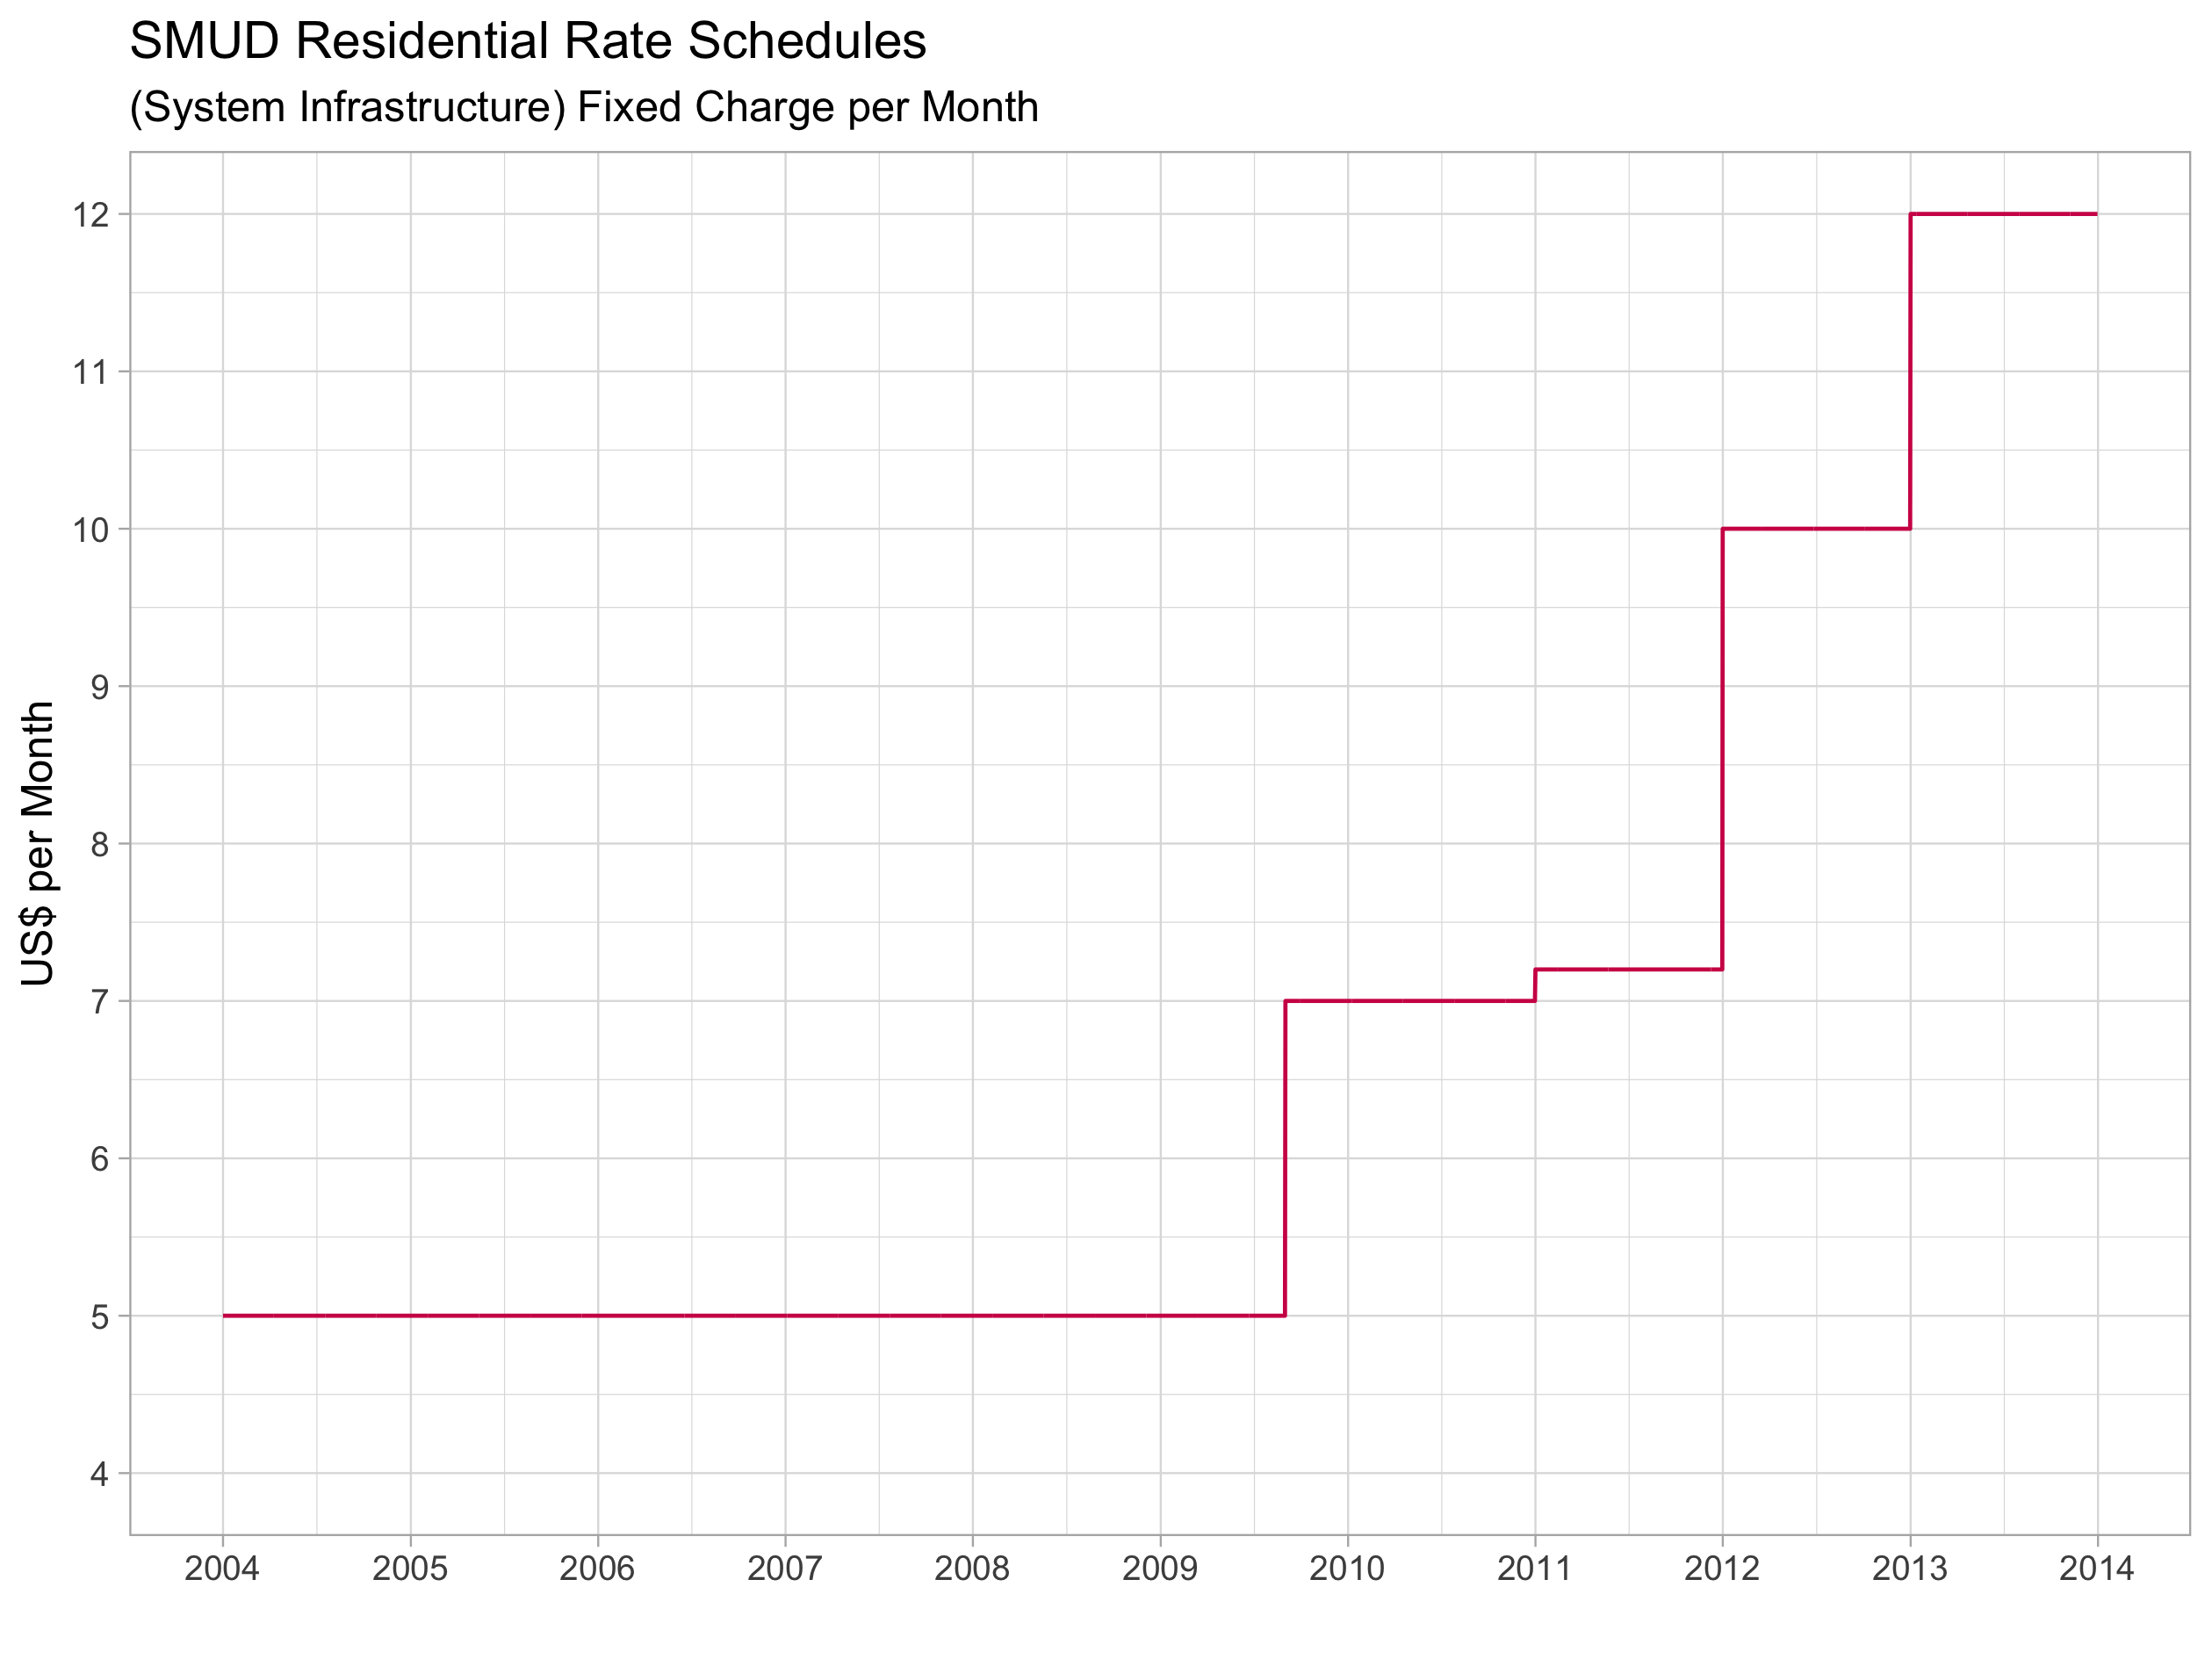
\includegraphics[scale = 0.18]{02_Plots/SMUD-Residential-Rate-Schedules_Fixed-Charge}
    \caption{SMUD Residential Rate Schedules: (System Infrastructure) Fixed Charge per Month}
%   \subcaption*{\textit{Notes: }}
    \label{Figure:Residential-Rate-Schedules_Fixed-Charge}
\end{figure}

\clearpage
\begin{figure}
    \centering
    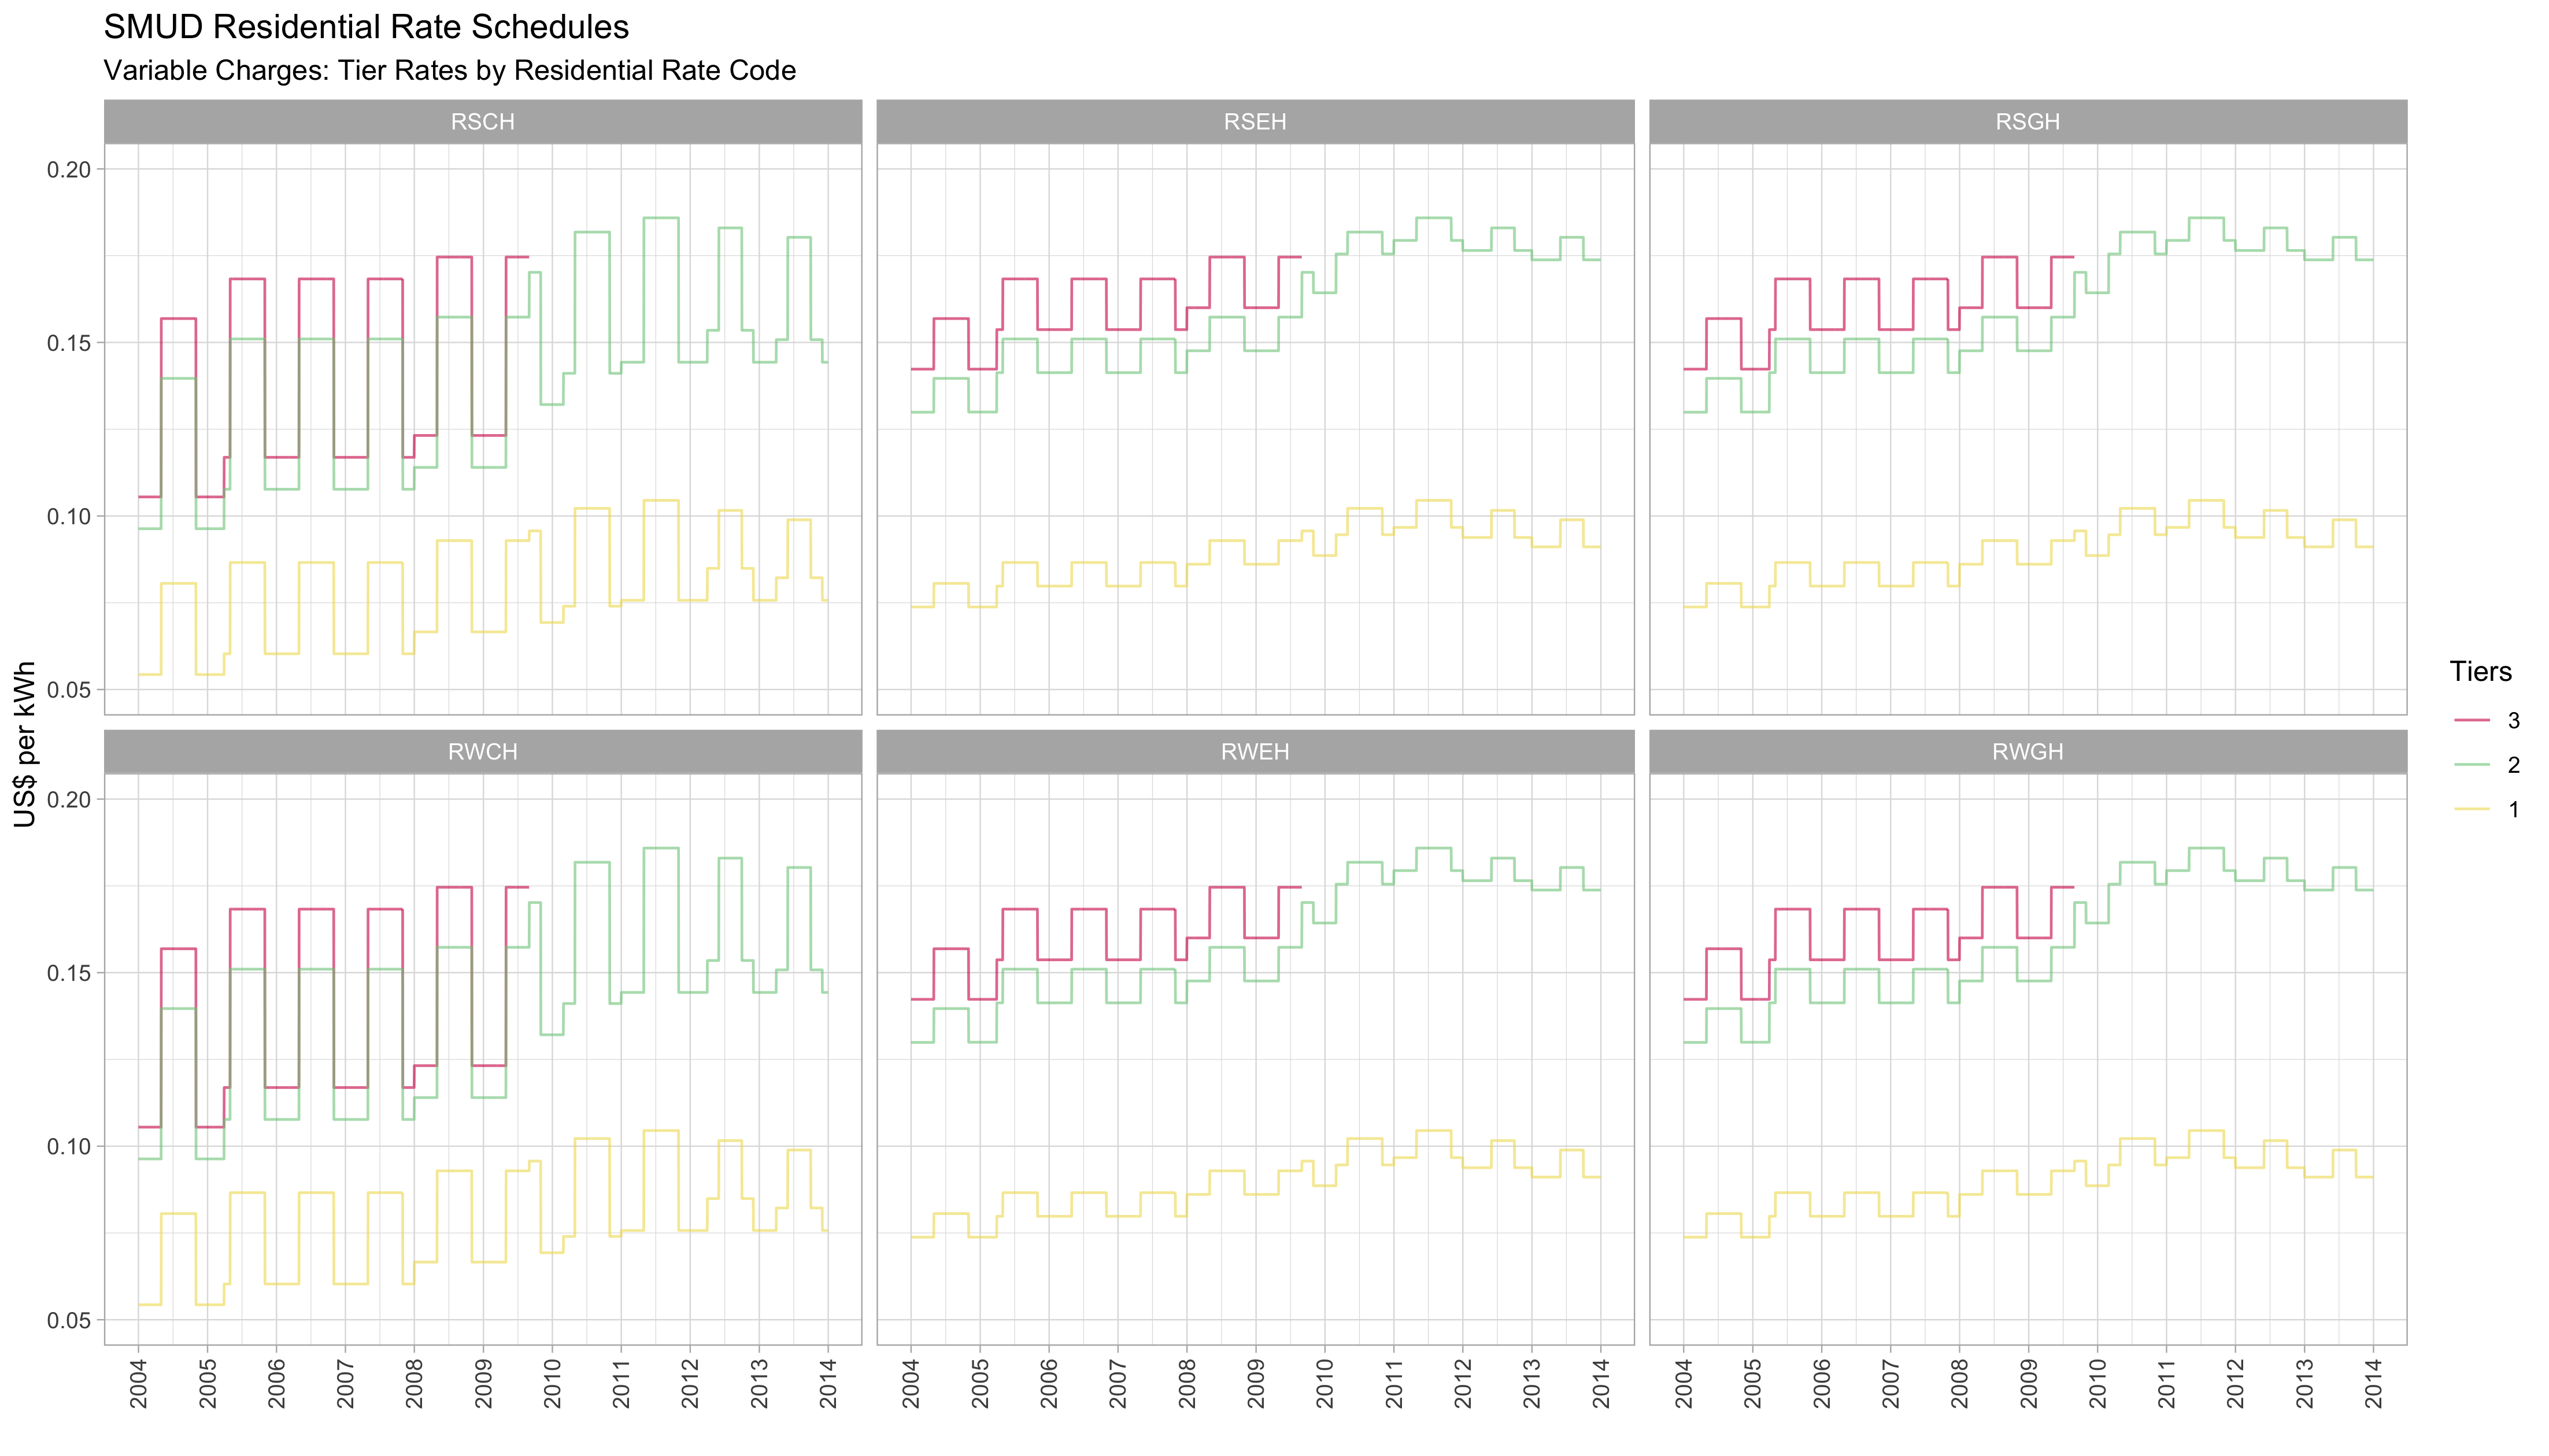
\includegraphics[scale = 0.105]{02_Plots/SMUD-Residential-Rate-Schedules_Variable-Charge_Normalized-Rate-Codes}
    \caption{SMUD Residential Rate Schedules: Variable Charges, By Residential Rate Code}
%   \subcaption*{\textit{Notes: }}
    \label{Figure:Residential-Rate-Schedules_Variable-Charges_By-Rate-Code}
\end{figure}
\vspace{0.3cm}

\begin{figure}
    \centering
    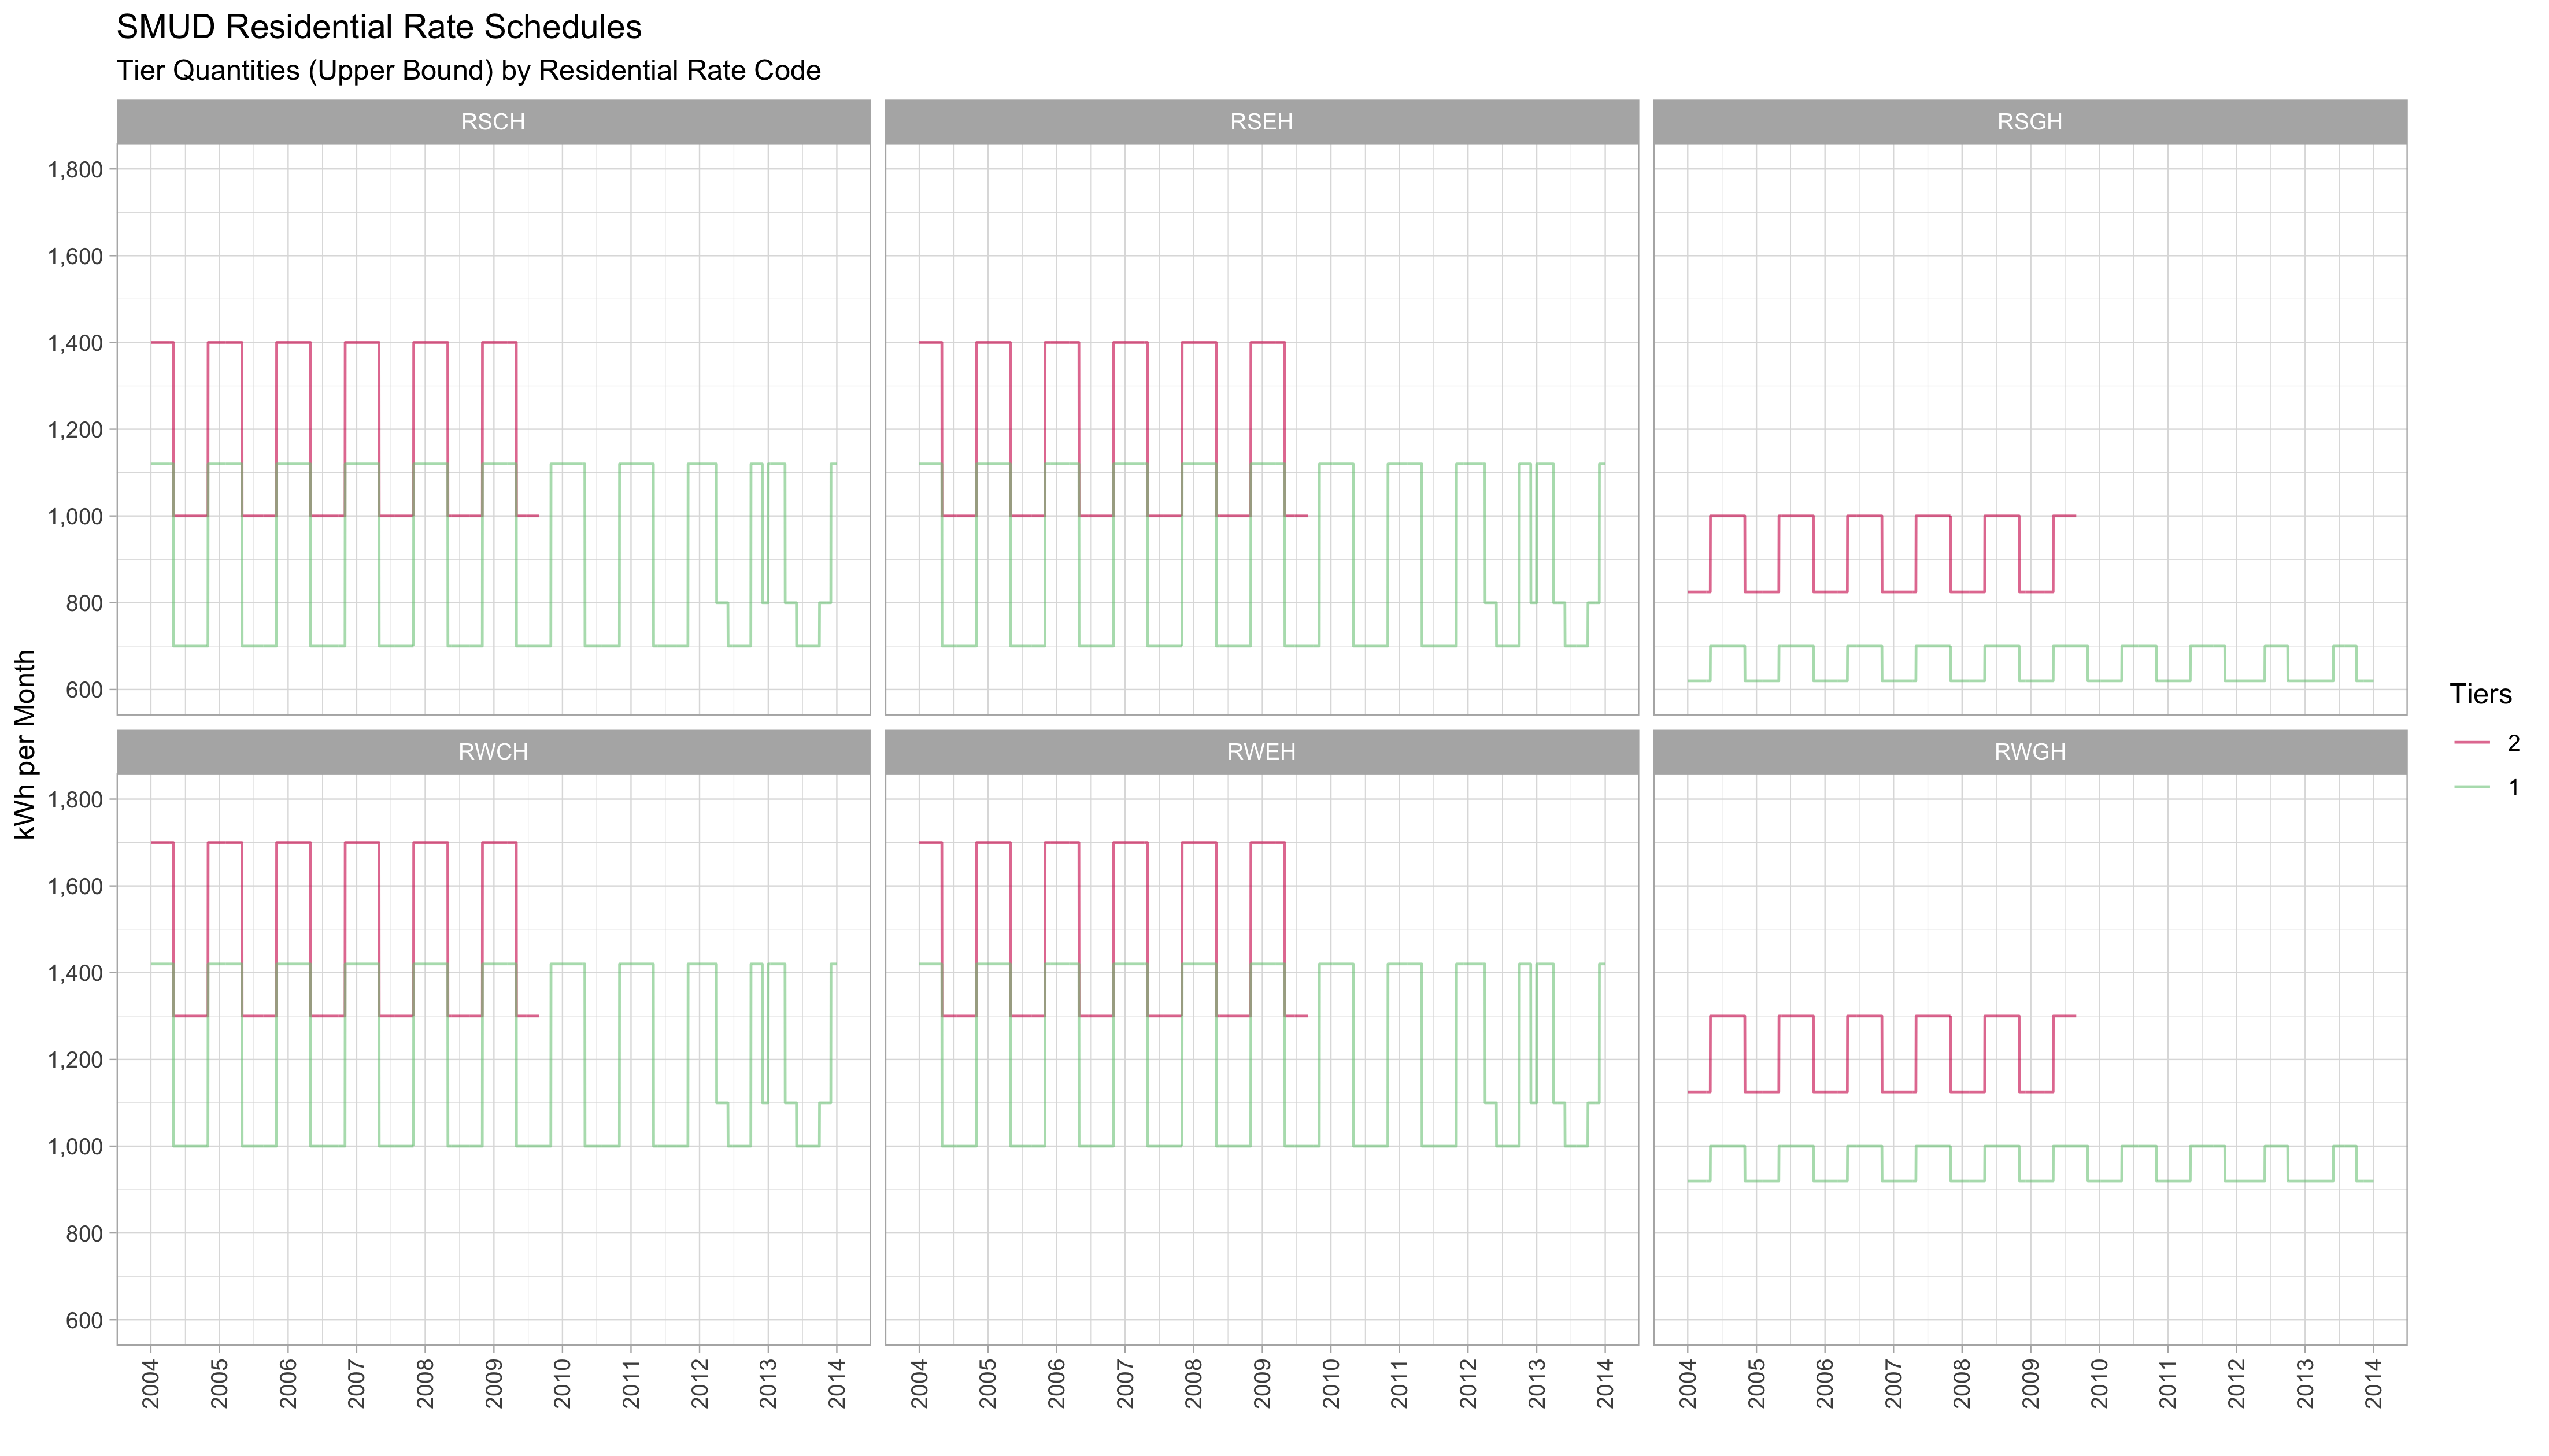
\includegraphics[scale = 0.105]{02_Plots/SMUD-Residential-Rate-Schedules_Qty_Normalized-Rate-Codes}
    \caption{SMUD Residential Rate Schedules: Base Usage Qty, By Residential Rate Code}
%   \subcaption*{\textit{Notes: }}
    \label{Figure:Residential-Rate-Schedules_Base-Usage-Qty_By-Rate-Code}
\end{figure}


\subsection{Scatter Plots}
\subsubsection{Un-Restricted Samples}
\begin{figure}
    \centering
    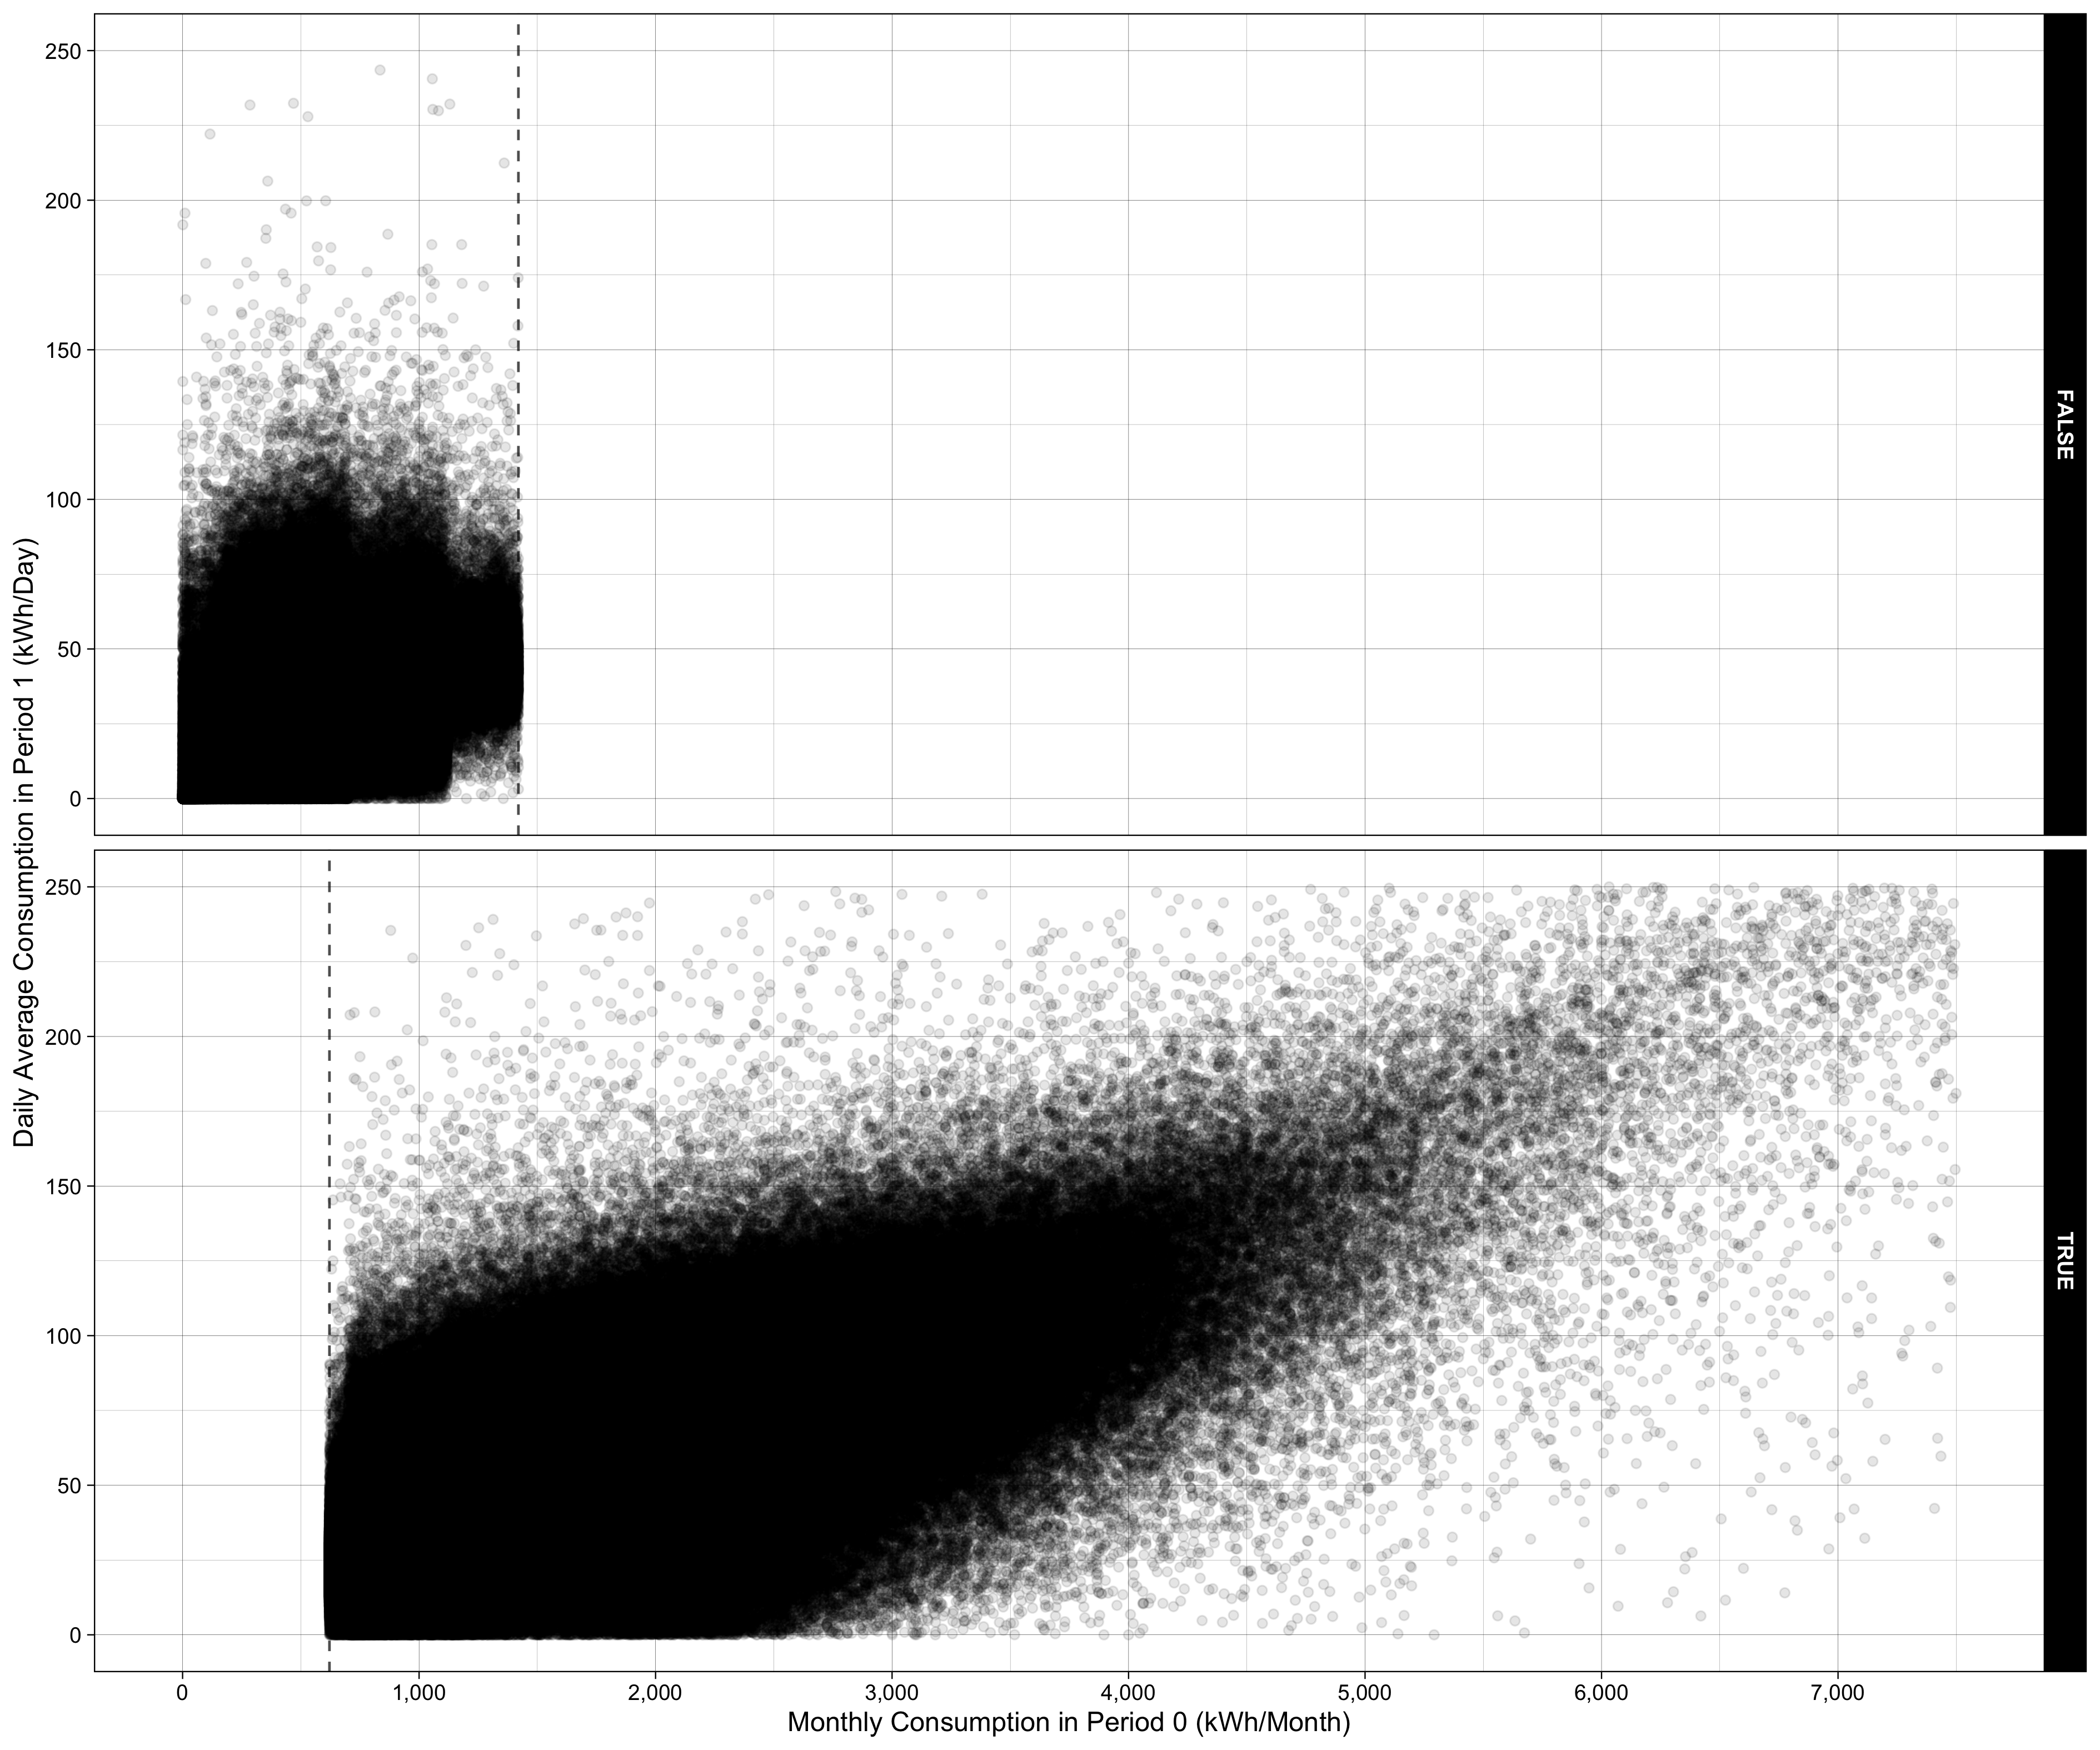
\includegraphics[scale = 0.13]{02_Plots/SMUD-Billing-Data_RD-Design_Scatter_Absolute-Consumption-in-H-Axis}
    \caption{Scatter Plot by Treatment Status}
    \subcaption*{\textit{Notes}: Horizontal axis is monthly consumption in period 0 (kWh/Month). The overlap in monthly consumption between control and treatment groups is due to seasonal changes in Base Usage Qty, as illustrated in Figure \ref{Figure:Residential-Rate-Schedules_Base-Usage-Qty_By-Rate-Code}.}
    \label{Figure:Scatter-Plots_Absolute-Values}
\end{figure}

\clearpage
\begin{figure}
    \centering
    \includegraphics[scale = 0.083]{02_Plots/SMUD-Billing-Data_RD-Design_Scatter_Spline-Fittings_Excluding-Outliers}
    \caption{Scatter Plots with Spline Fits}
   \subcaption*{\textit{Notes}: Horizontal axis is normalized consumption in period 0 relative to Base Usage Qty (\%).}
    \label{Figure:Scatter-Plots-with-Splie-Fits}
\end{figure}


\clearpage
\subsubsection{Samples constructed based on Rate Codes}
\vspace{0.2cm}

\begin{figure}
    \begin{subfigure}{1.0\textwidth}
        \centering
        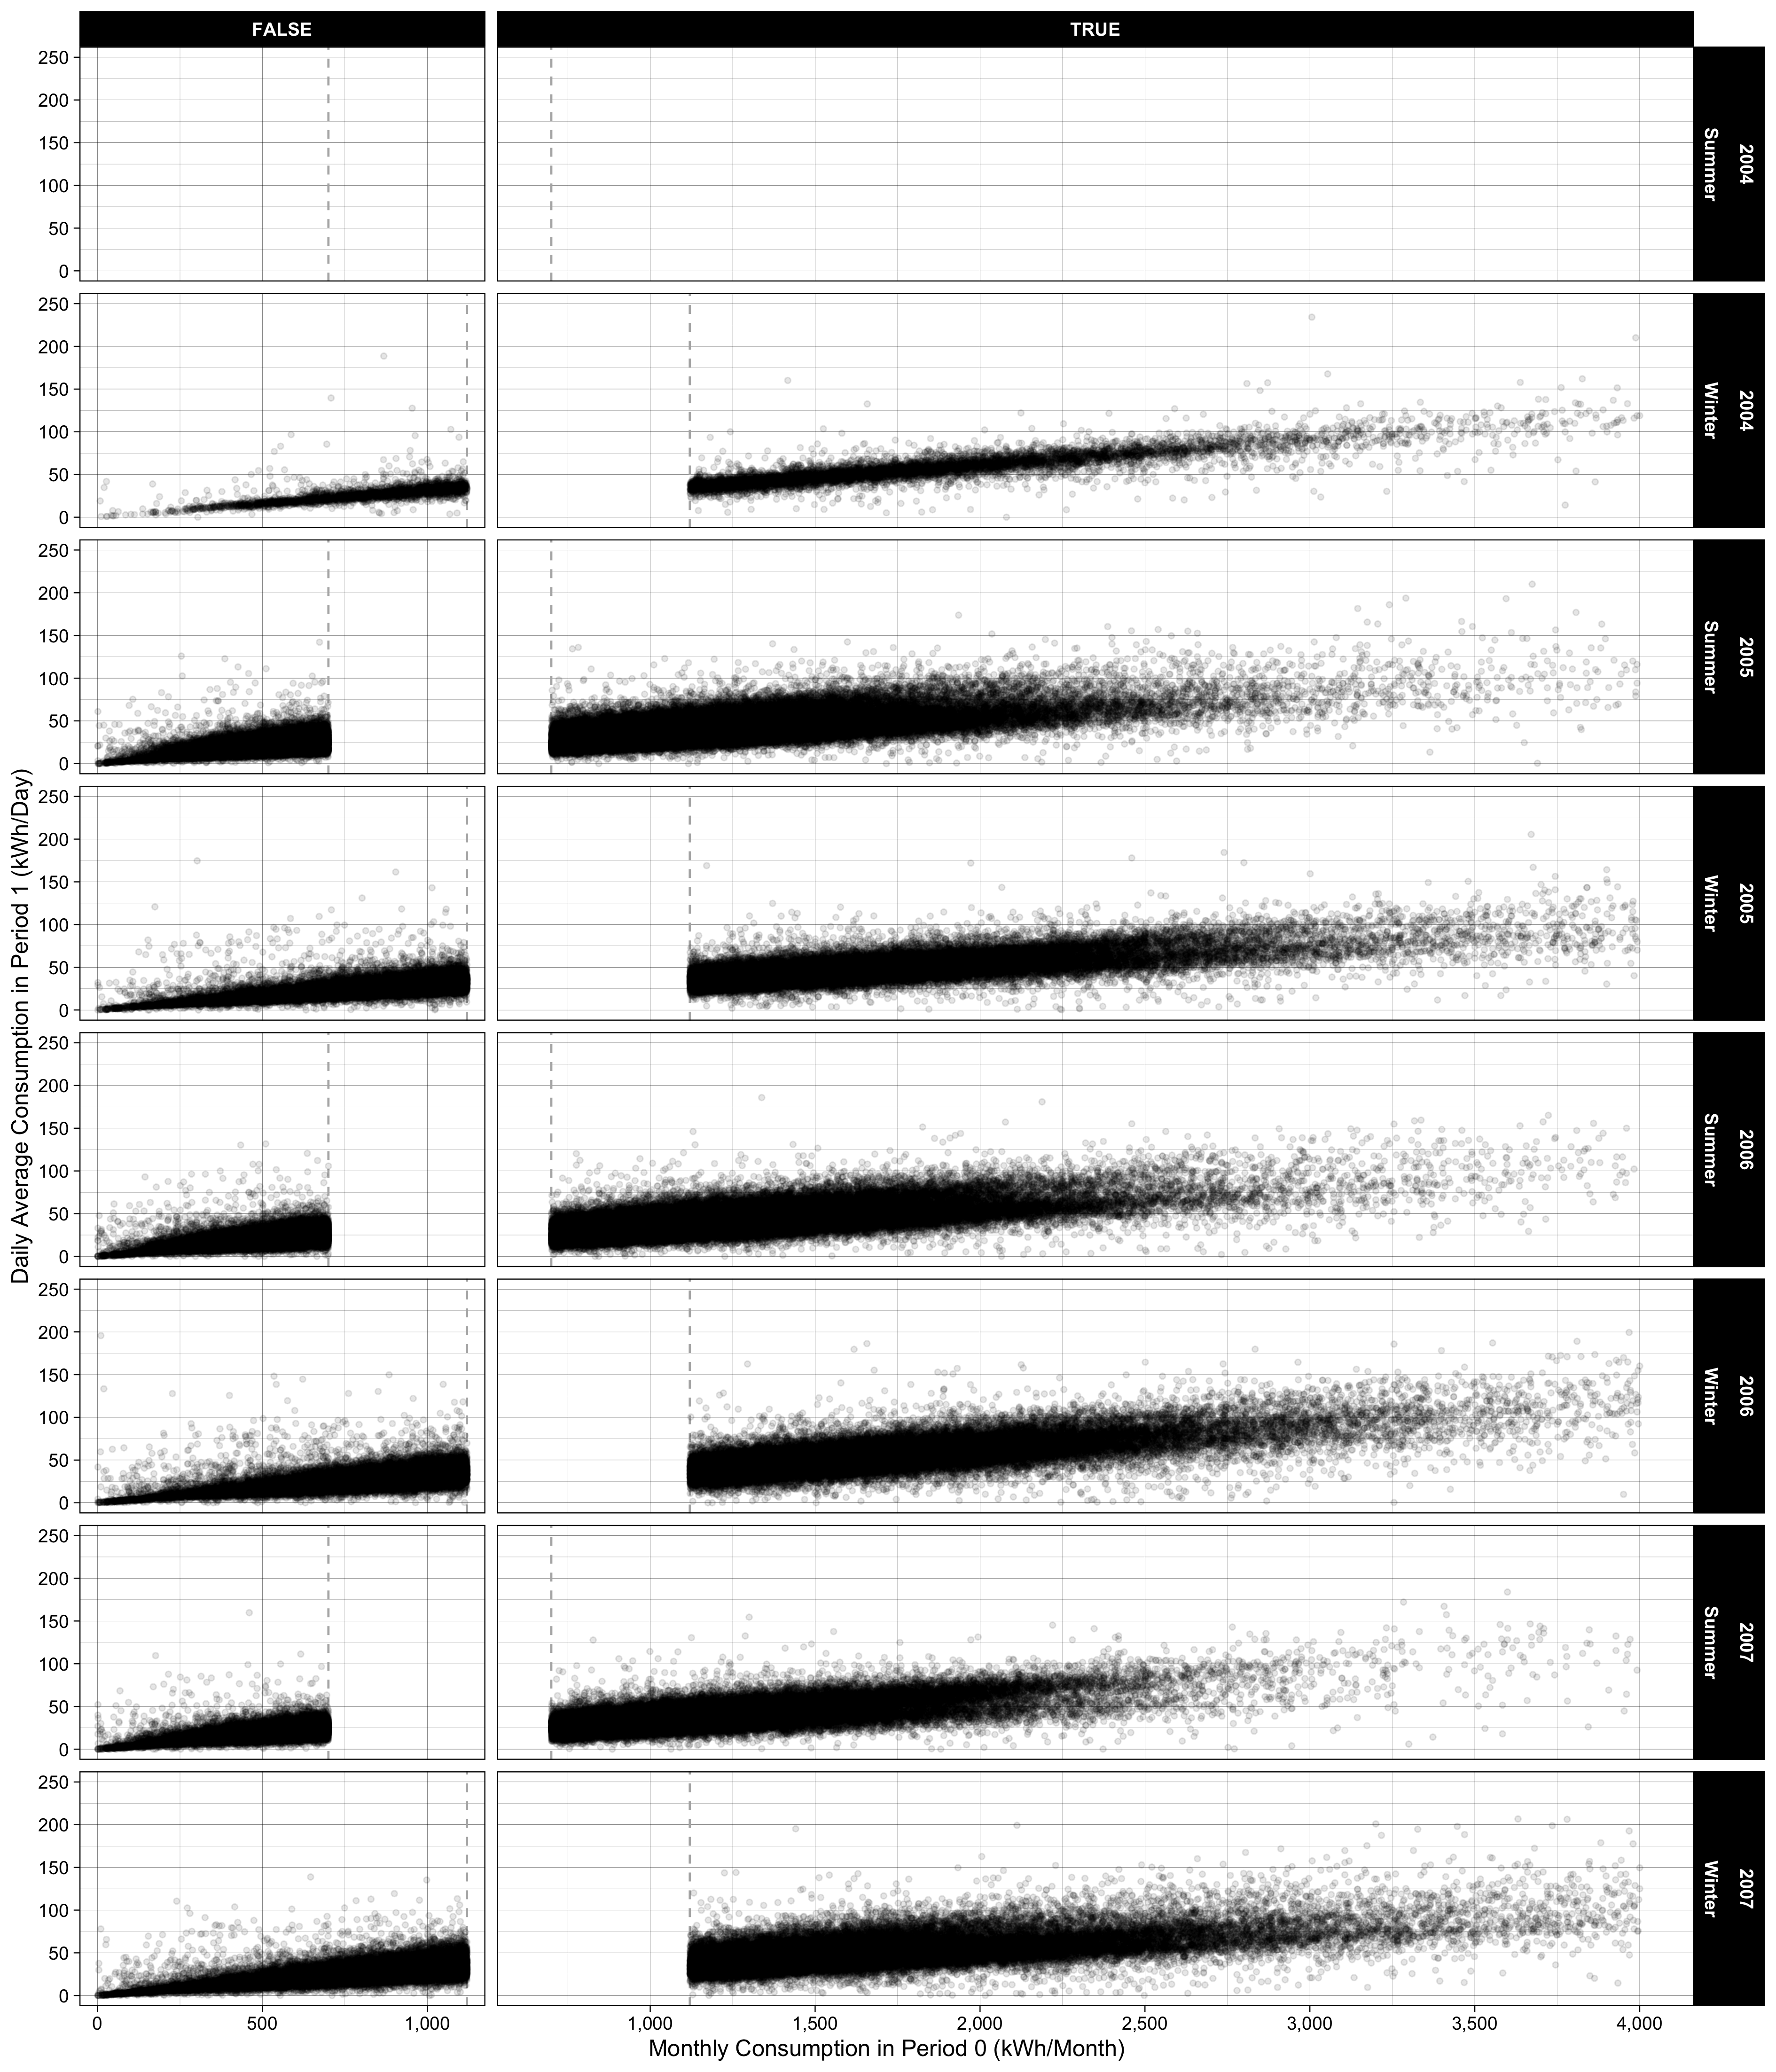
\includegraphics[scale = 0.12]{02_Plots/SMUD-Billing-Data_RD-Design_Scatter_Absolute-Consumption-in-H-Axis_RSCH_2004-2007}
        \caption{Observations between 2004 and 2007}
    \end{subfigure}
    \newline
    \begin{subfigure}{1.0\textwidth}
        \centering
        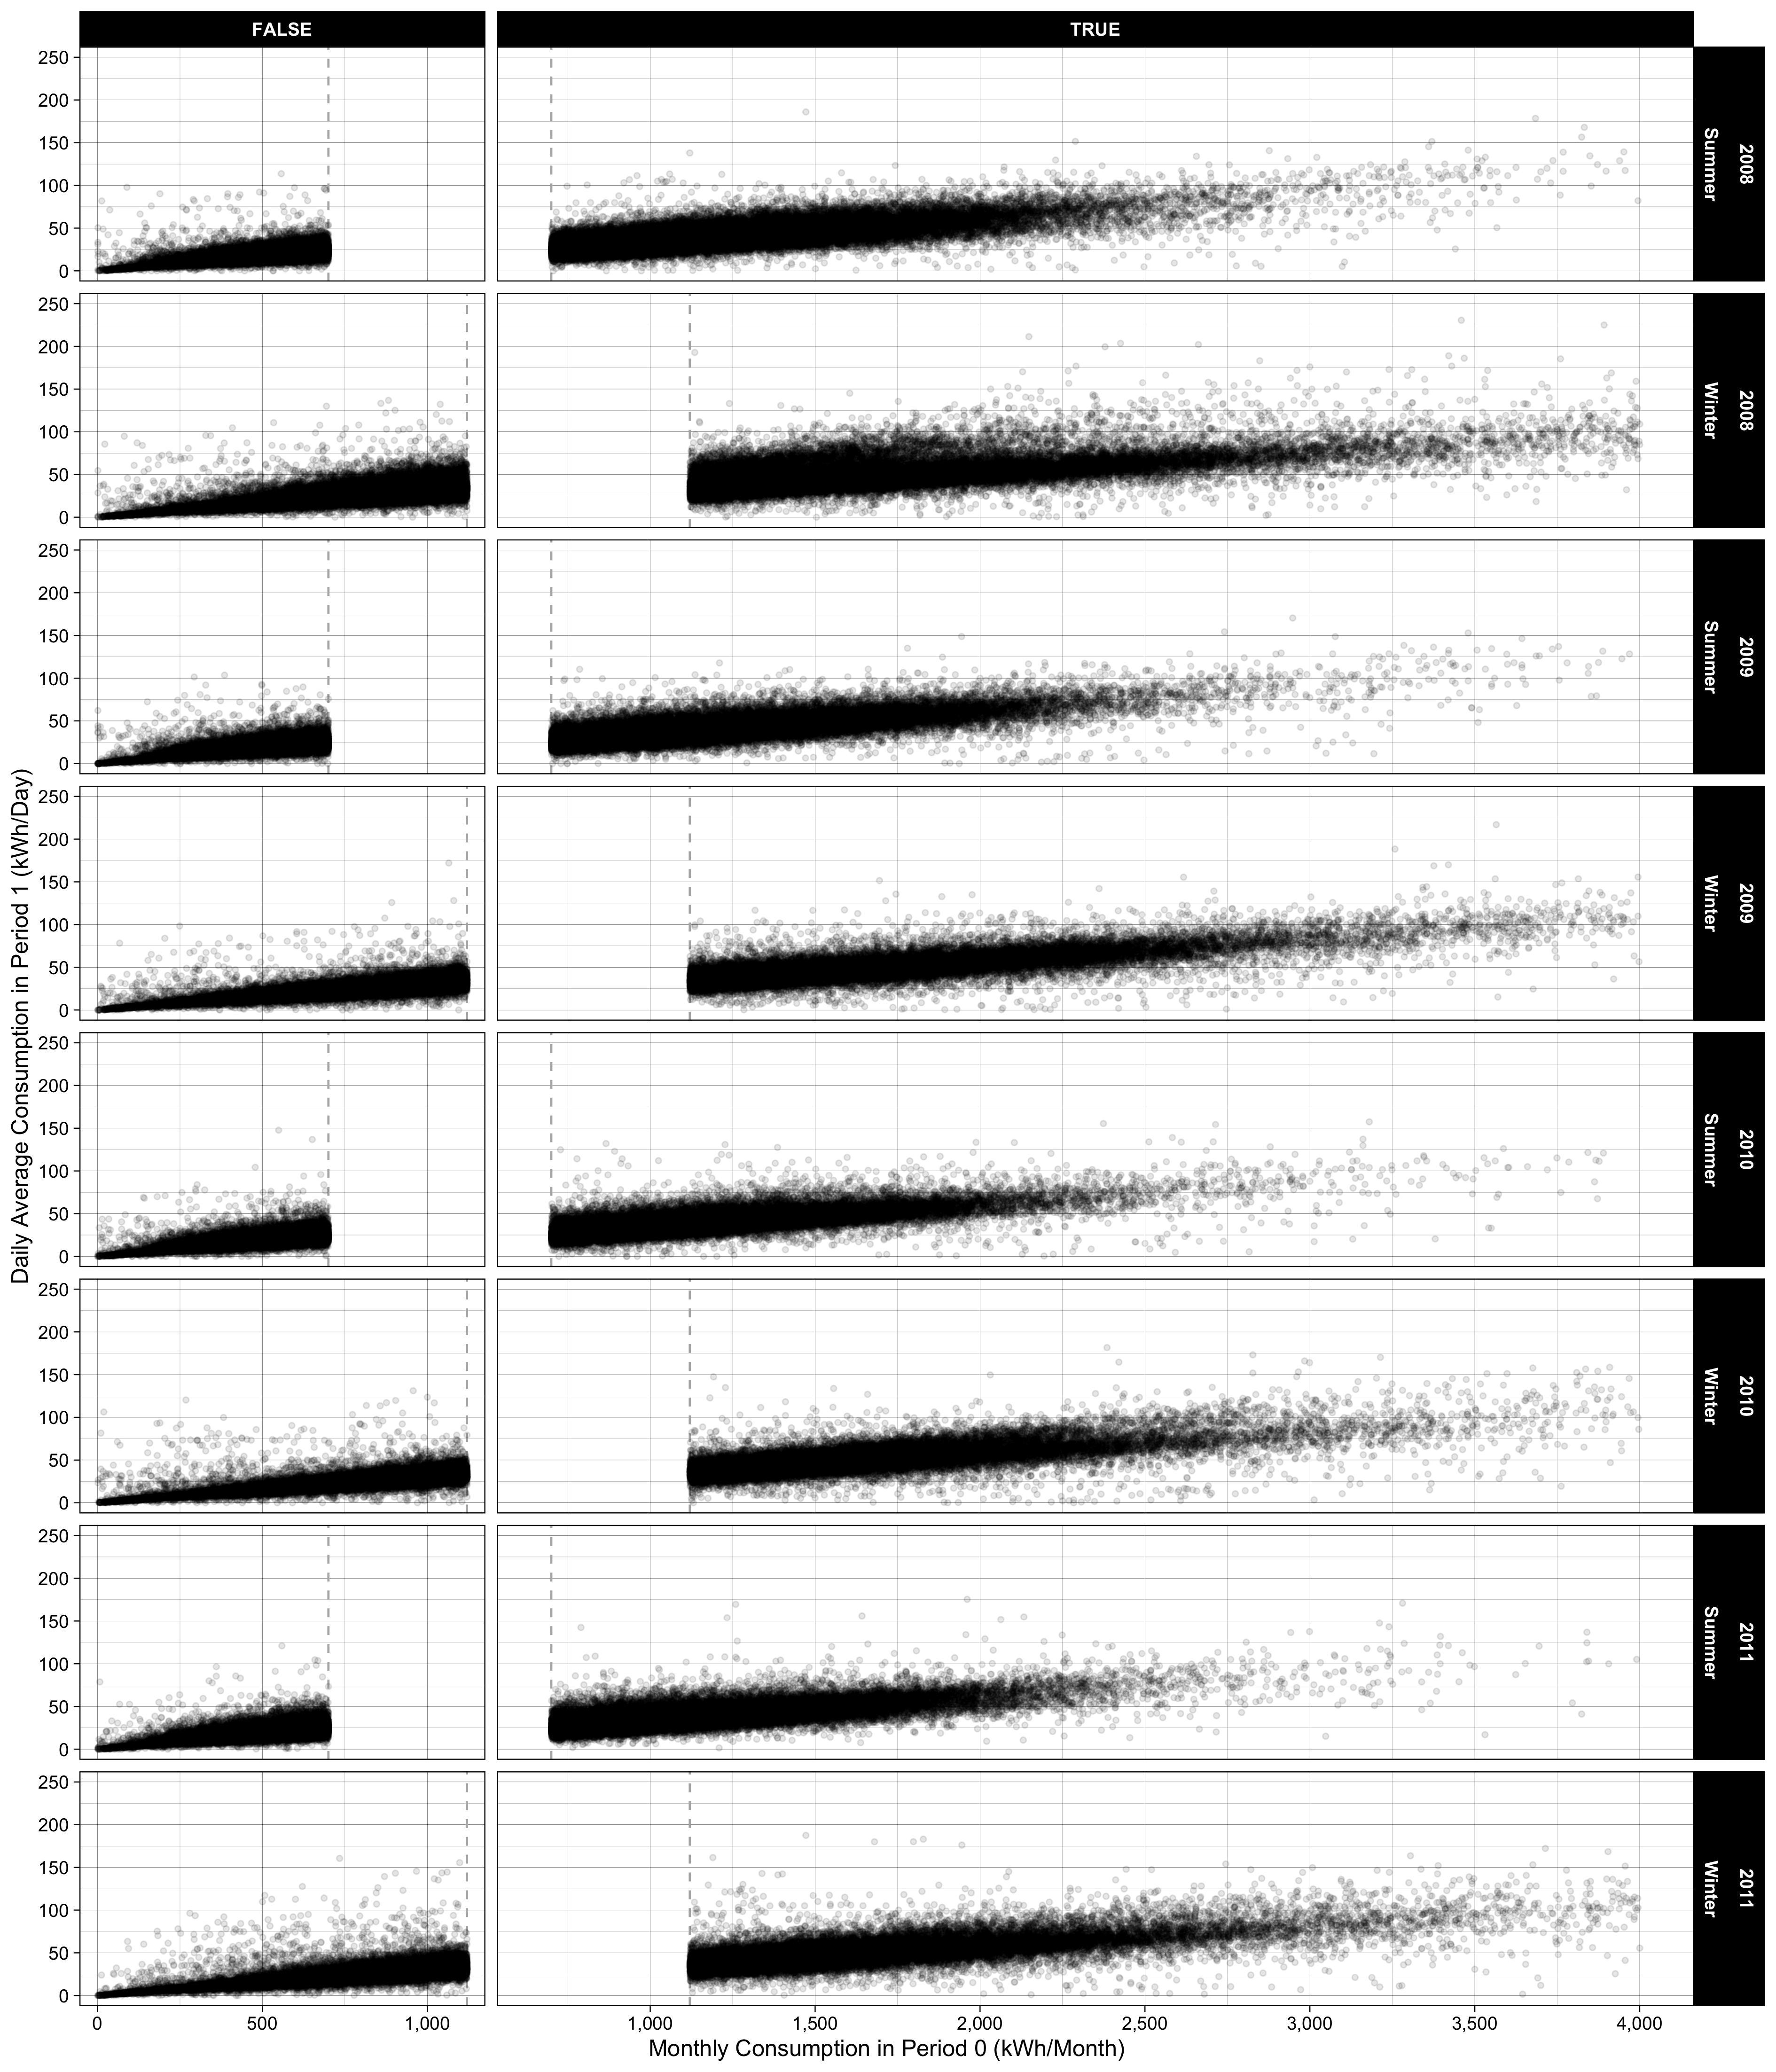
\includegraphics[scale = 0.12]{02_Plots/SMUD-Billing-Data_RD-Design_Scatter_Absolute-Consumption-in-H-Axis_RSCH_2008-2011}
        \caption{Observations between 2008 and 2011}
    \end{subfigure}
    \caption{Scatter Plots by Treatment Status, Year, and Season: For RSCH}
   \subcaption*{\textit{Notes}: Horizontal axis is normalized consumption in period 0 relative to Base Usage Qty (\%). The vertical dashed lines indicate the Base Usage Qty in corresponding year and season.}
    \label{Figure:Scatter-Plots_RSCH}
\end{figure}

\clearpage
\begin{figure}
    \begin{subfigure}{1.0\textwidth}
        \centering
        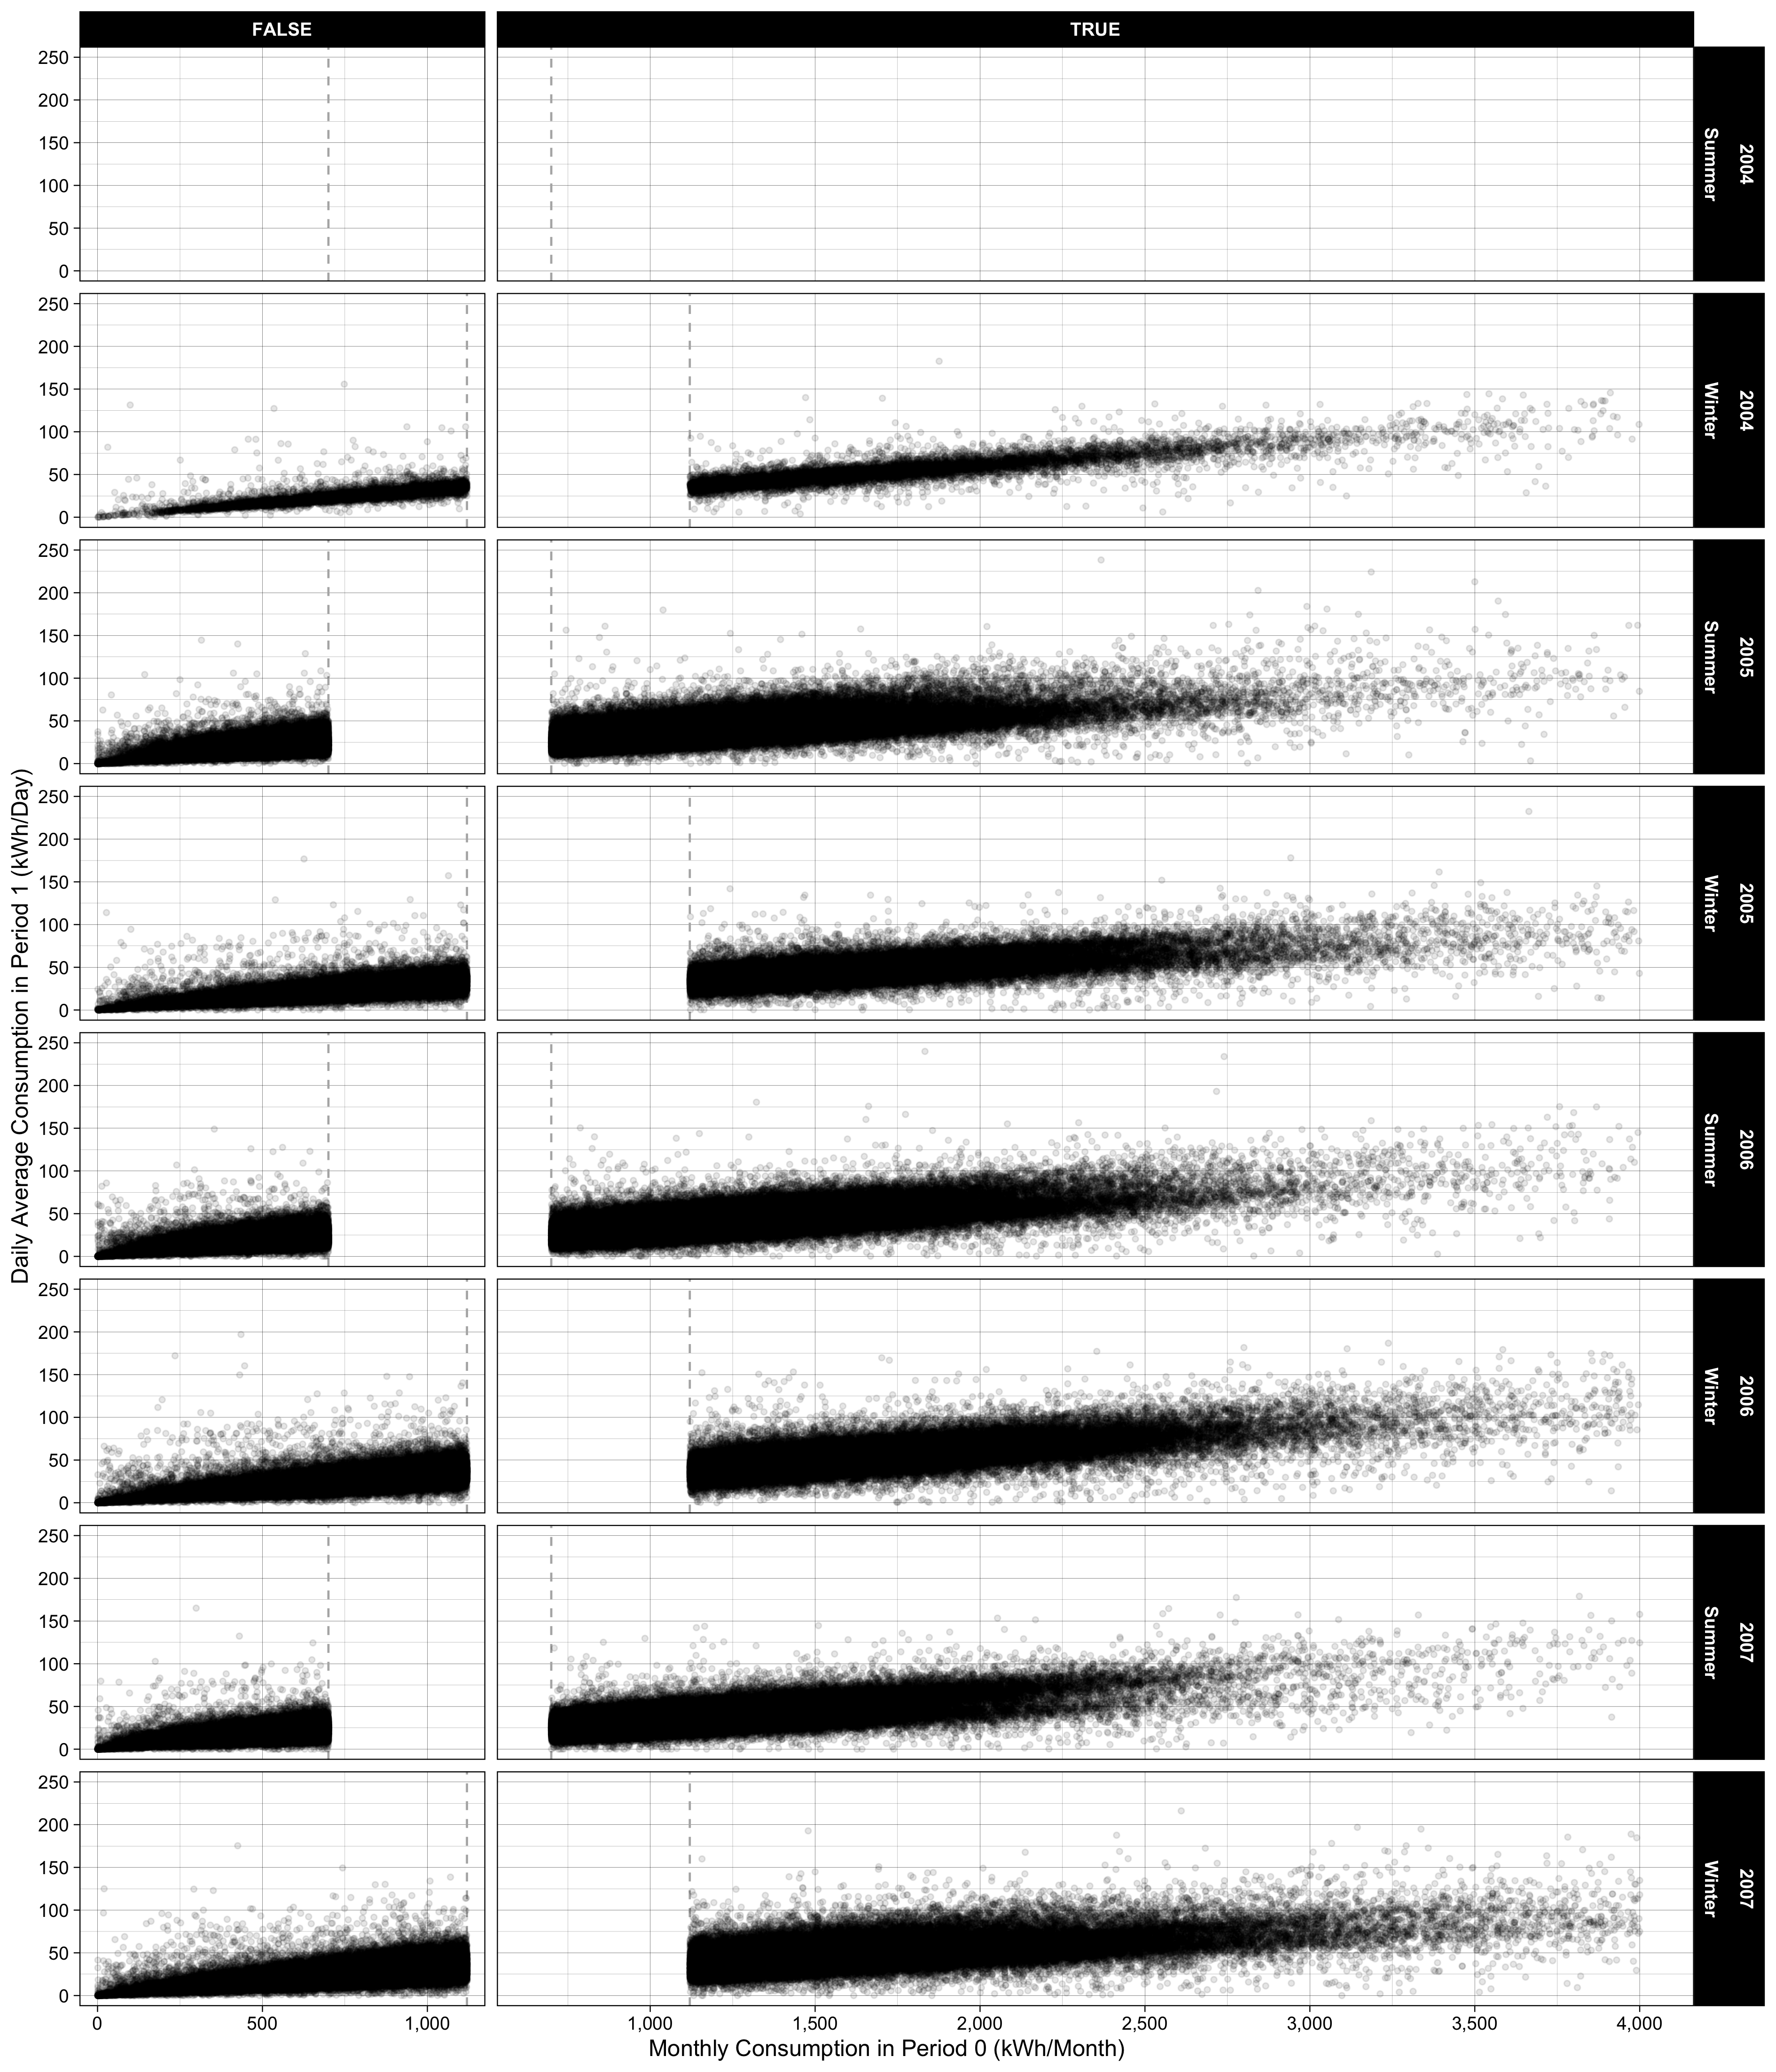
\includegraphics[scale = 0.12]{02_Plots/SMUD-Billing-Data_RD-Design_Scatter_Absolute-Consumption-in-H-Axis_RSEH_2004-2007}
        \caption{Observations between 2004 and 2007}  
    \end{subfigure}
    \begin{subfigure}{1.0\textwidth}
        \centering
        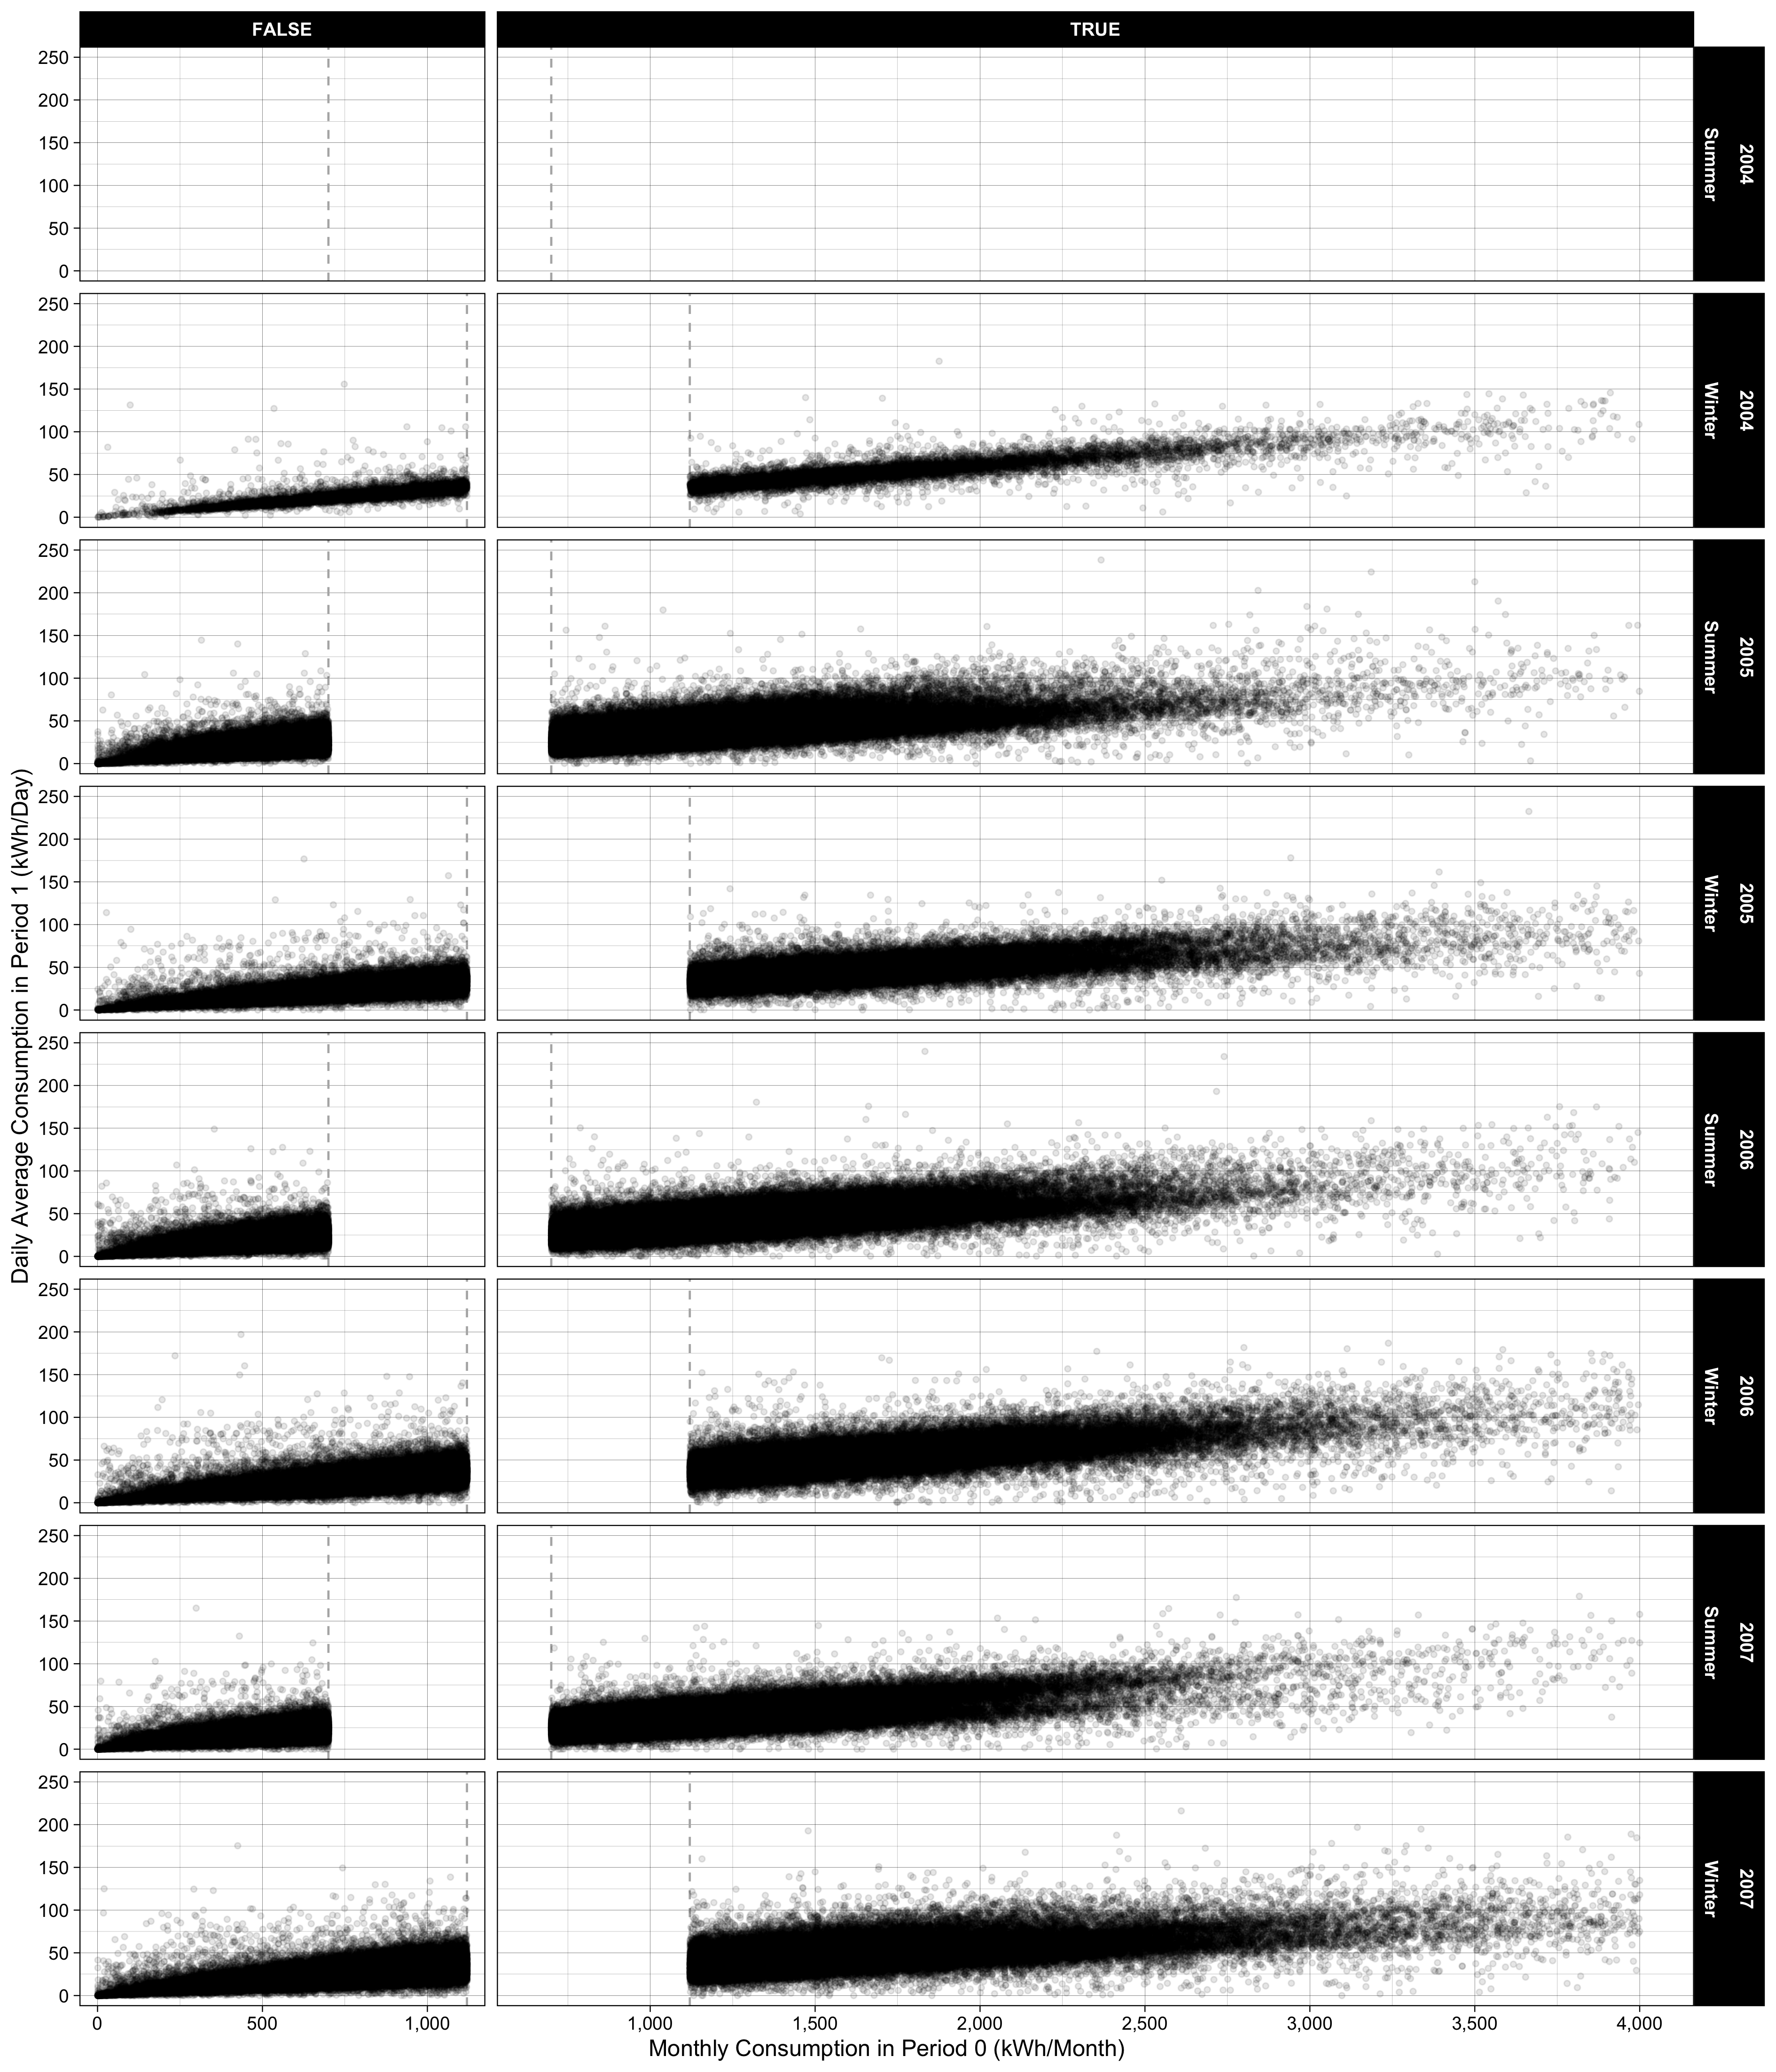
\includegraphics[scale = 0.12]{02_Plots/SMUD-Billing-Data_RD-Design_Scatter_Absolute-Consumption-in-H-Axis_RSEH_2004-2007}
        \caption{Observations between 2008 and 2011}  
    \end{subfigure}
    \caption{Scatter Plots by Treatment Status, Year, and Season: For RSEH}
    \subcaption*{\textit{Notes}: Horizontal axis is normalized consumption in period 0 relative to Base Usage Qty (\%). The vertical dashed lines indicate the Base Usage Qty in corresponding year and season.}
    \label{Figure:Scatter-Plots_RSEH}
\end{figure}

\clearpage
\begin{figure}
    \begin{subfigure}{1.0\textwidth}
        \centering
        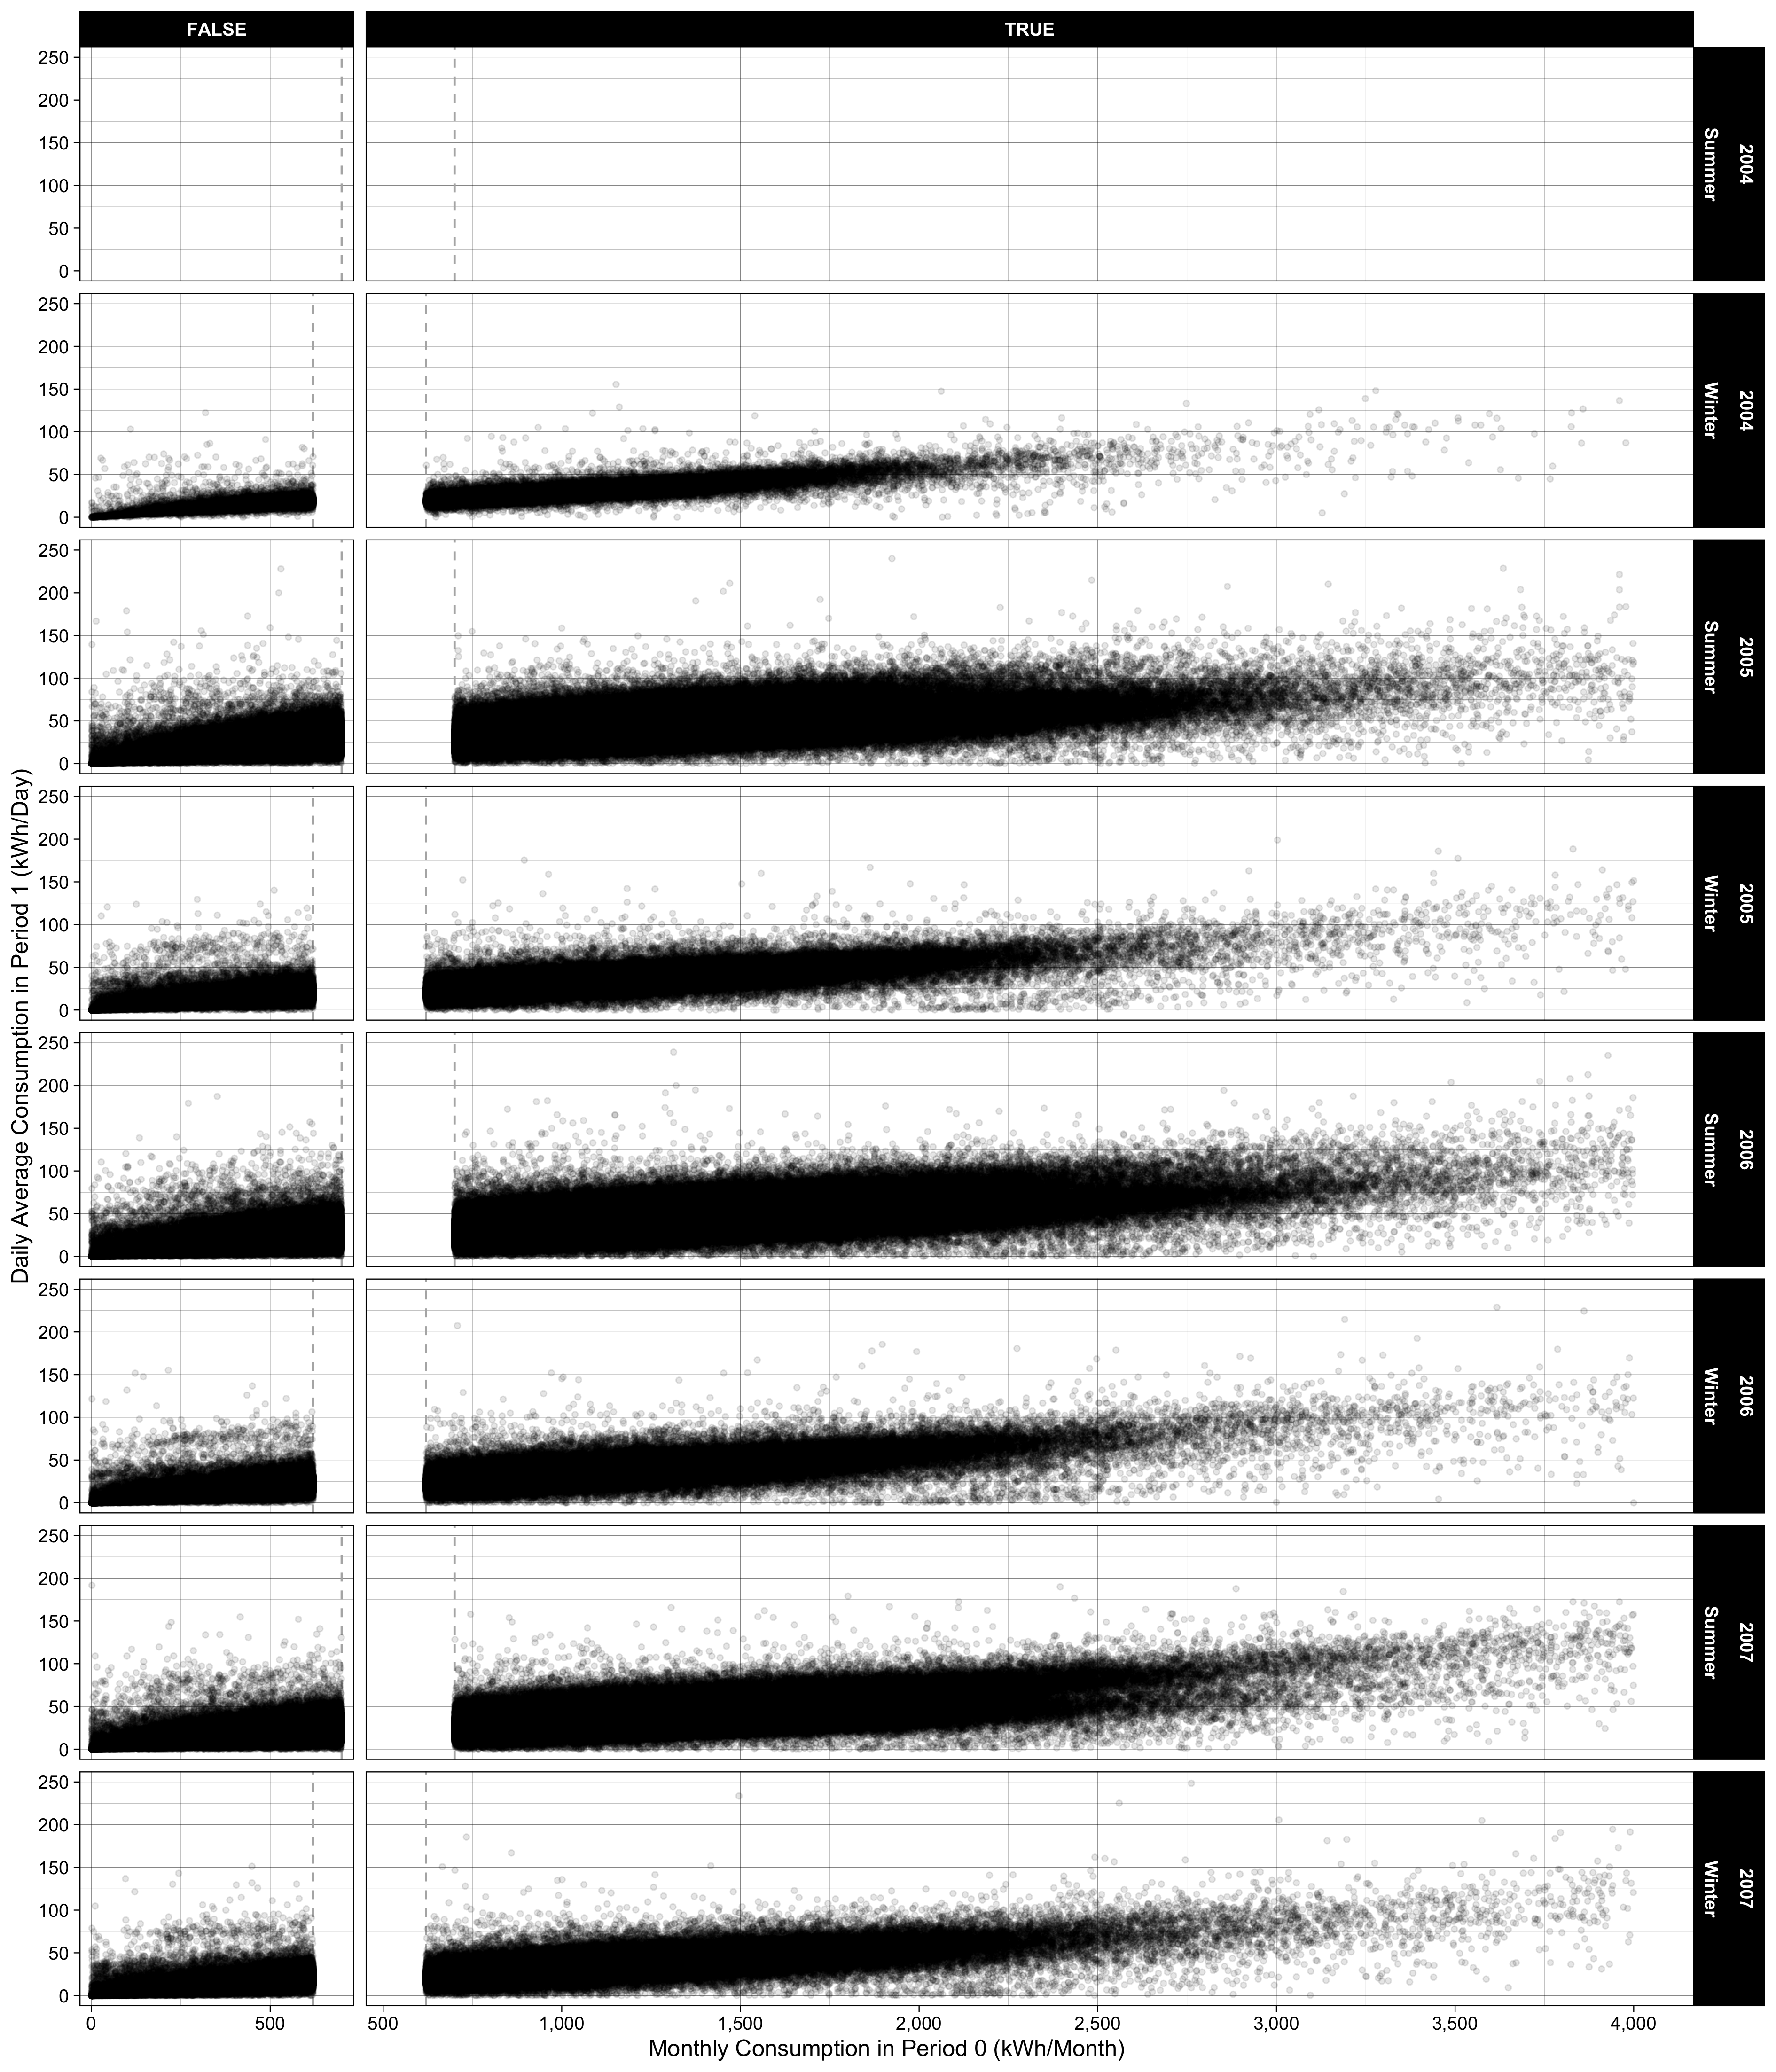
\includegraphics[scale = 0.12]{02_Plots/SMUD-Billing-Data_RD-Design_Scatter_Absolute-Consumption-in-H-Axis_RSGH_2004-2007}
        \caption{Observations between 2004 and 2007}
    \end{subfigure}
    \begin{subfigure}{1.0\textwidth}
        \centering
        \includegraphics[scale = 0.12]{02_Plots/SMUD-Billing-Data_RD-Design_Scatter_Absolute-Consumption-in-H-Axis_RSGH_2008-2011}
        \caption{Observations between 2008 and 2011}
    \end{subfigure}
    \caption{Scatter Plots by Treatment Status, Year, and Season: For RSGH}
    \subcaption*{\textit{Notes}: Horizontal axis is normalized consumption in period 0 relative to Base Usage Qty (\%). The vertical dashed lines indicate the Base Usage Qty in corresponding year and season.}
    \label{Figure:Scatter-Plots_RSGH_2004-2007}
\end{figure}


\clearpage
\subsection{Estimated Treatment Effects by Bandwidth}

\subsubsection{Un-Restricted Samples}
\begin{figure}
    \centering
    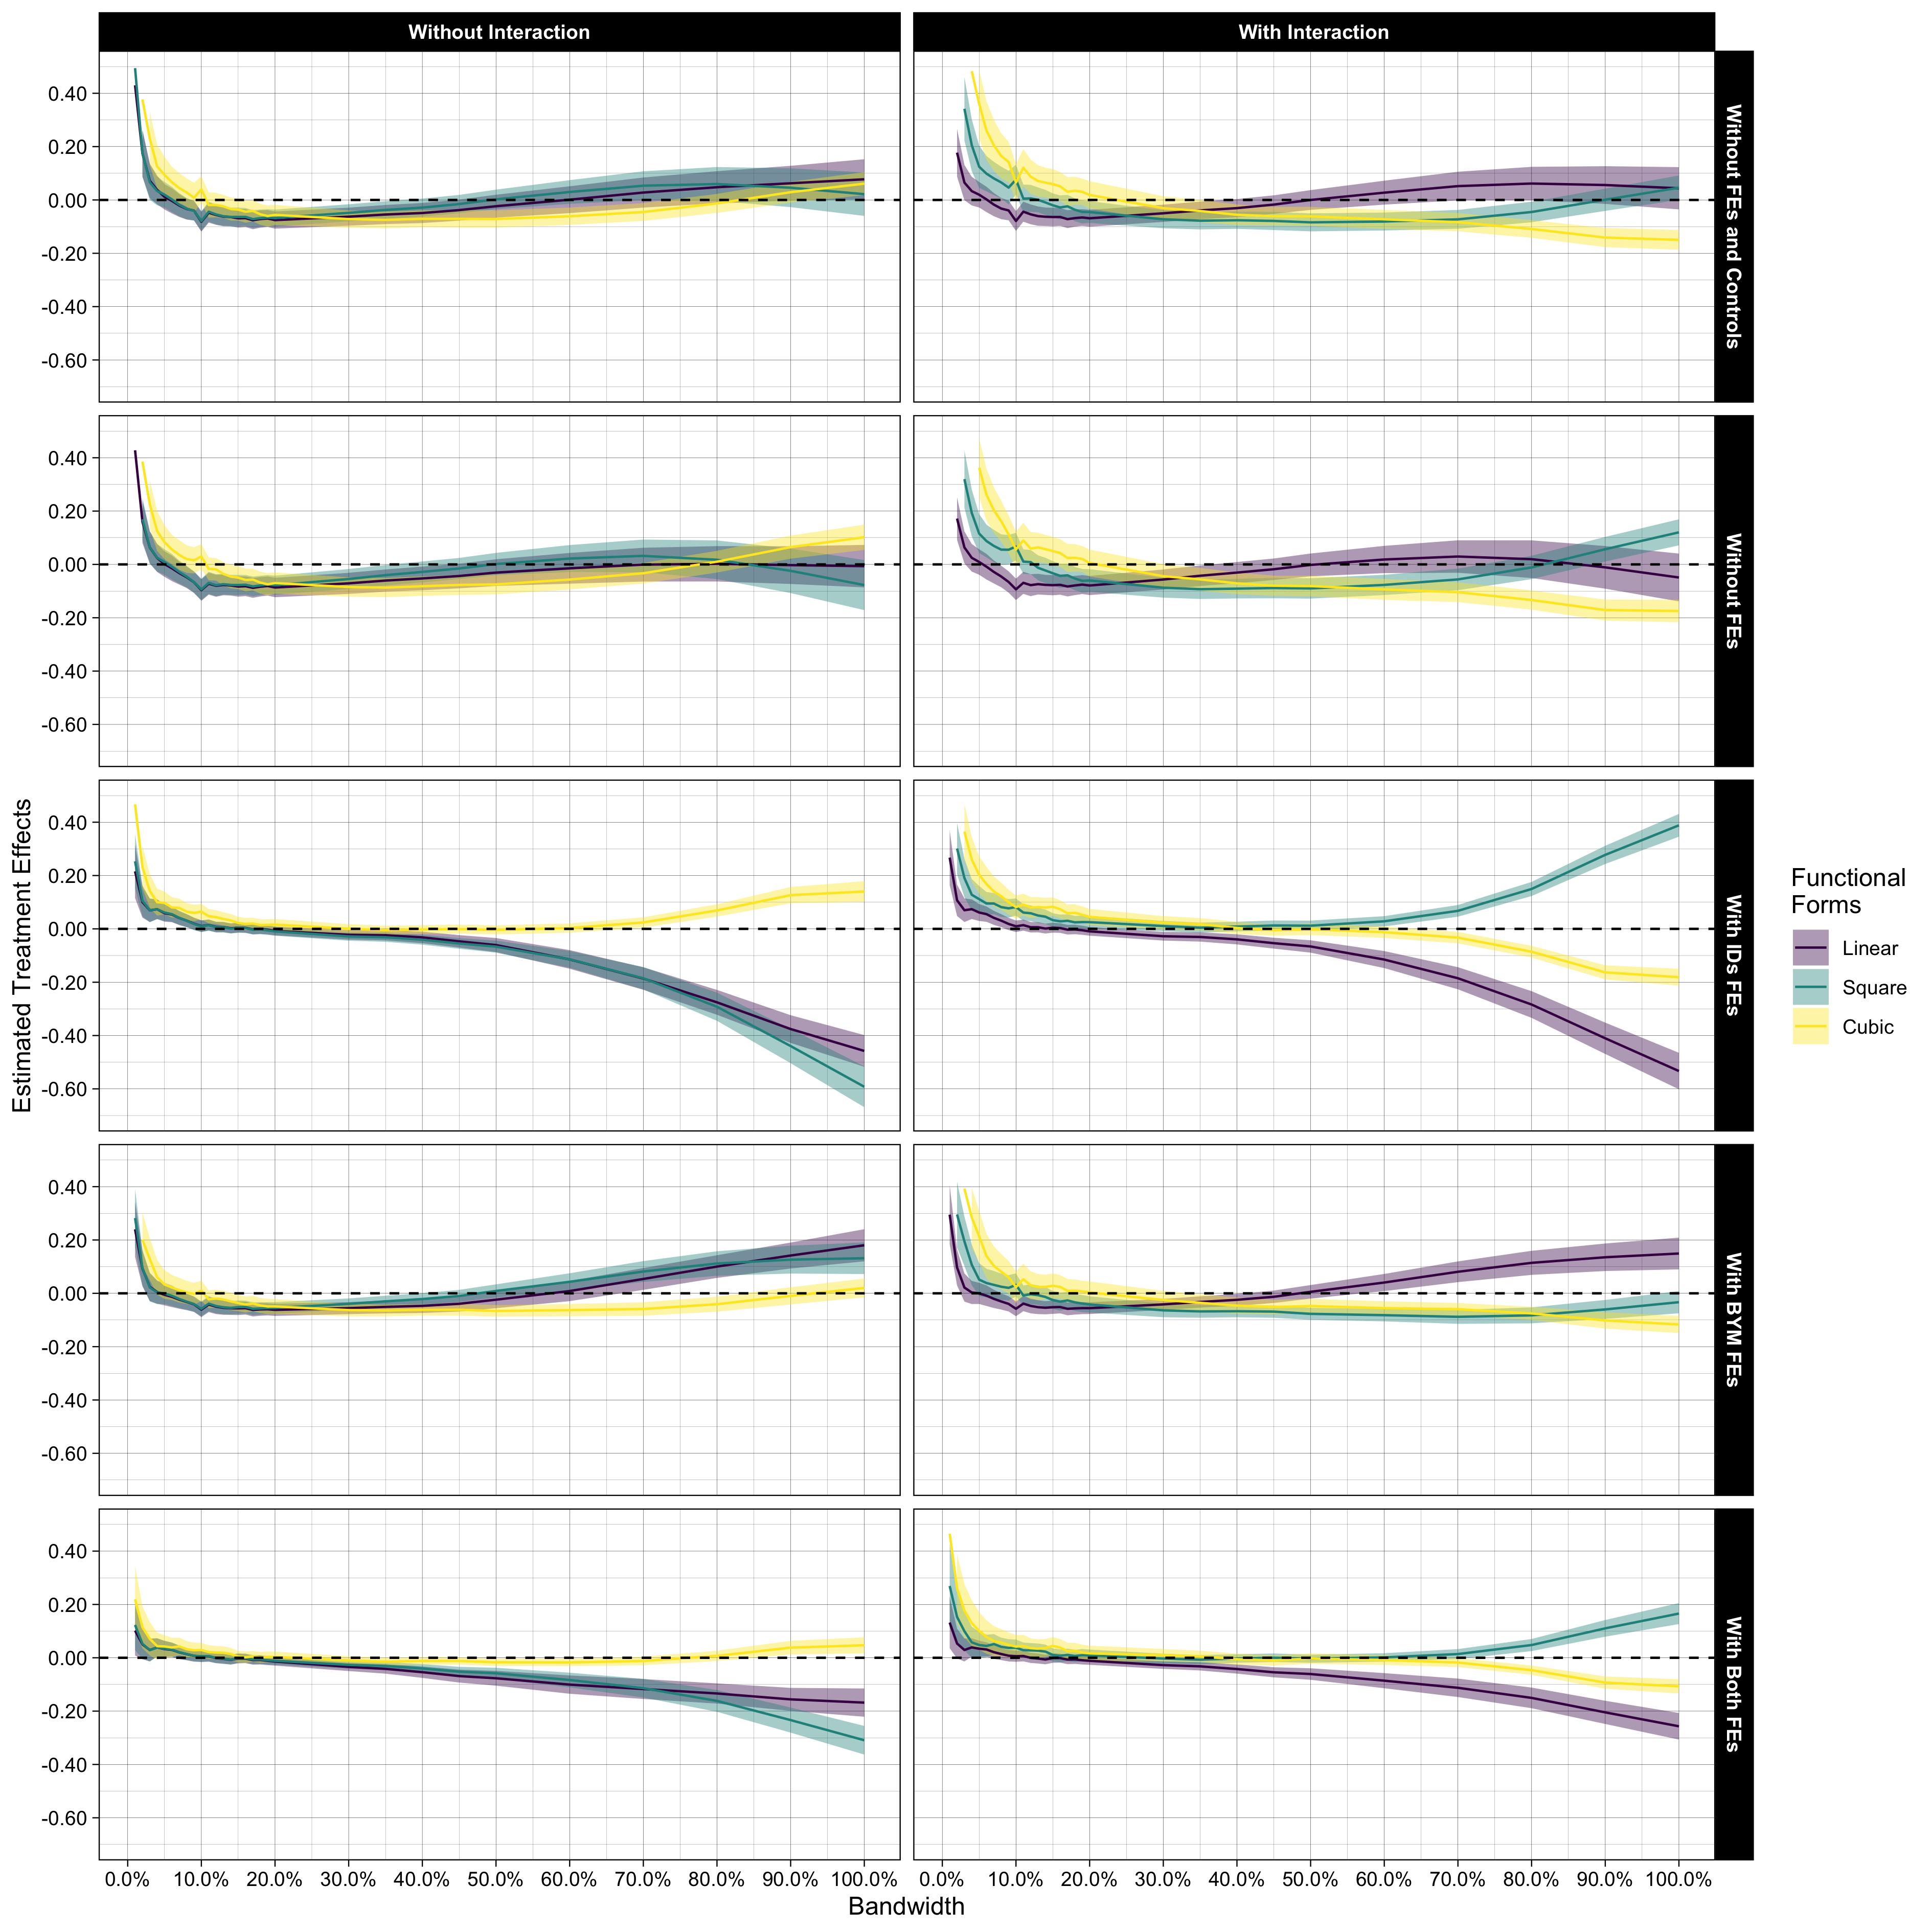
\includegraphics[scale = 0.13]{02_Plots/Regression-Results_RD-Design_Treatment-Effect-by-BW_All-Models}
    \caption{Estimated Treatment Effects by Bandwidth and Functional Form}
    \subcaption*{\textit{Notes}: Highest standard errors are selected between heteroskedasticity-robust and clustered (by Account-Premise IDs and Billing Year-Month) standard errors. Shaded areas in each panel indicate the 95\% confidence intervals.}
    \label{Figure:Estimated-Treatment-Effects_By-Functional-Form}
\end{figure}

\clearpage
\subsubsection{Samples constructed based on Rate Codes}
\begin{figure}
    \begin{subfigure}{1.0\textwidth}
        \centering
        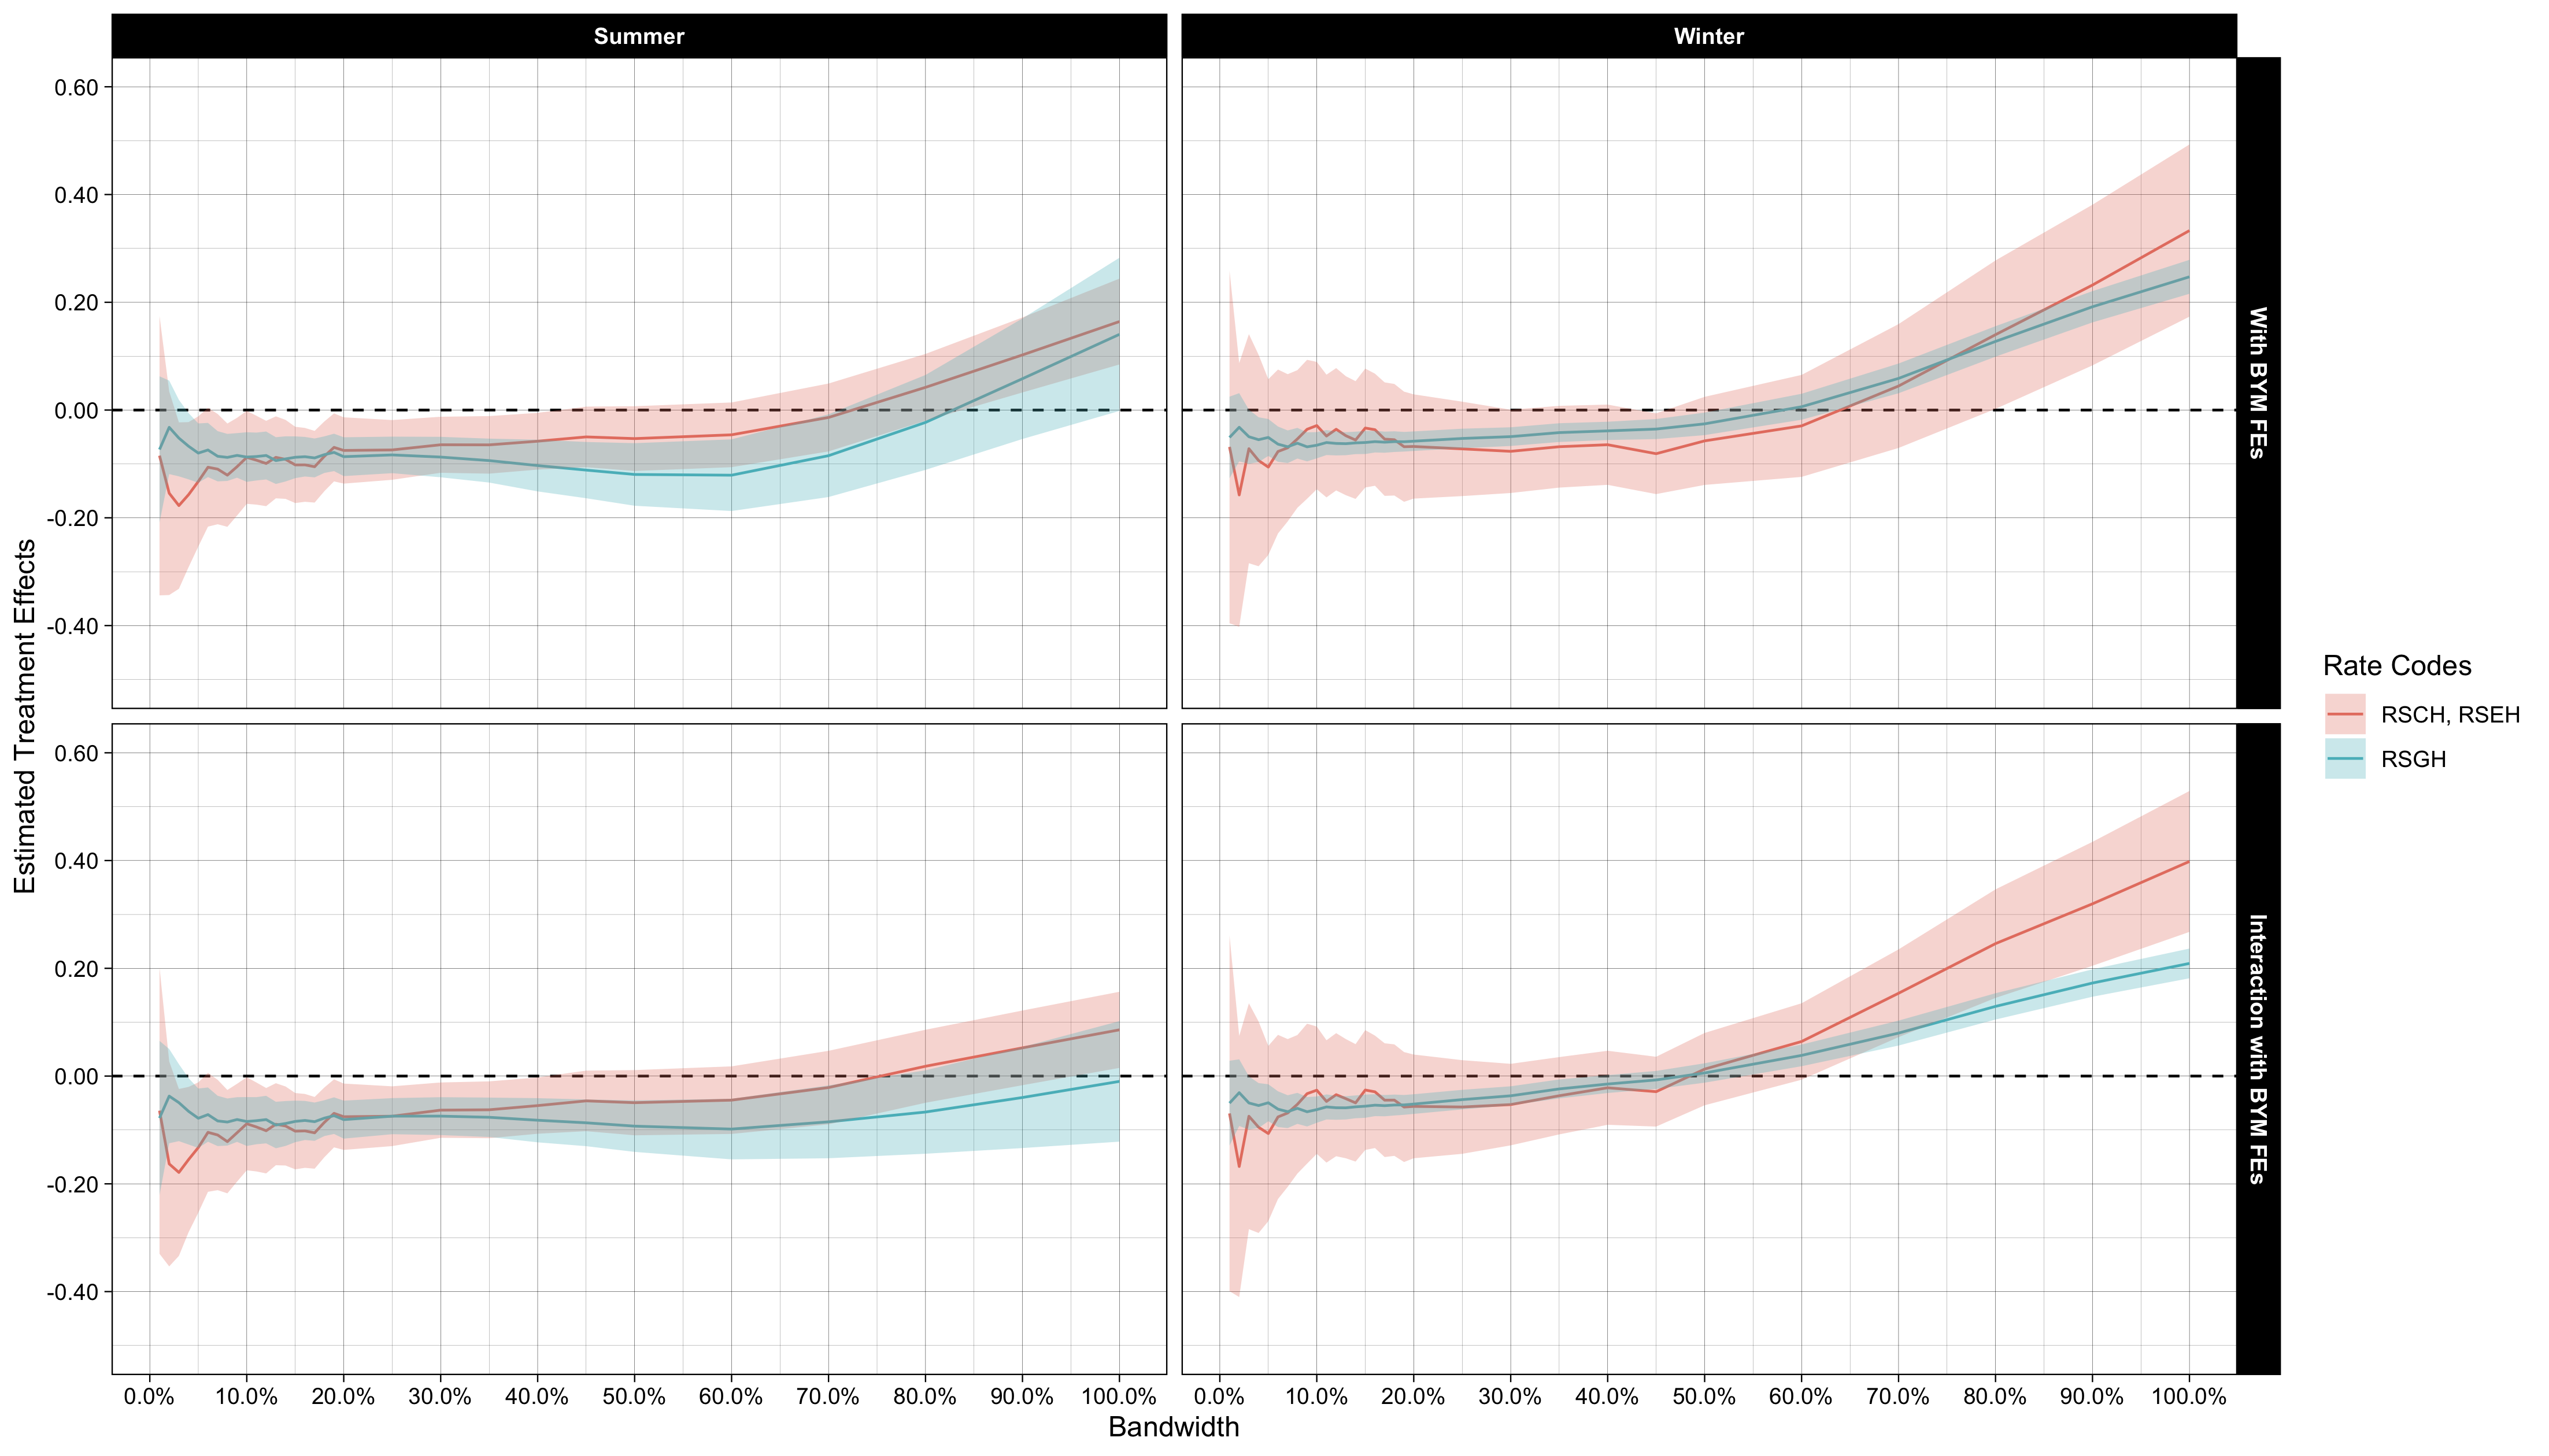
\includegraphics[scale = 0.108]{02_Plots/Regression-Results_RD-Design_Treatment-Effect-by-BW-and-Rate-Codes_Linear}
        \caption{Models with Linear Term of Running Variable}
        \label{Figure:Estimated-Treatment-Effects_By-Rate-Code-and-Season_Linear}
        \vspace{0.3cm}
    \end{subfigure}
    \newline
    \begin{subfigure}{1.0\textwidth}
        \centering
        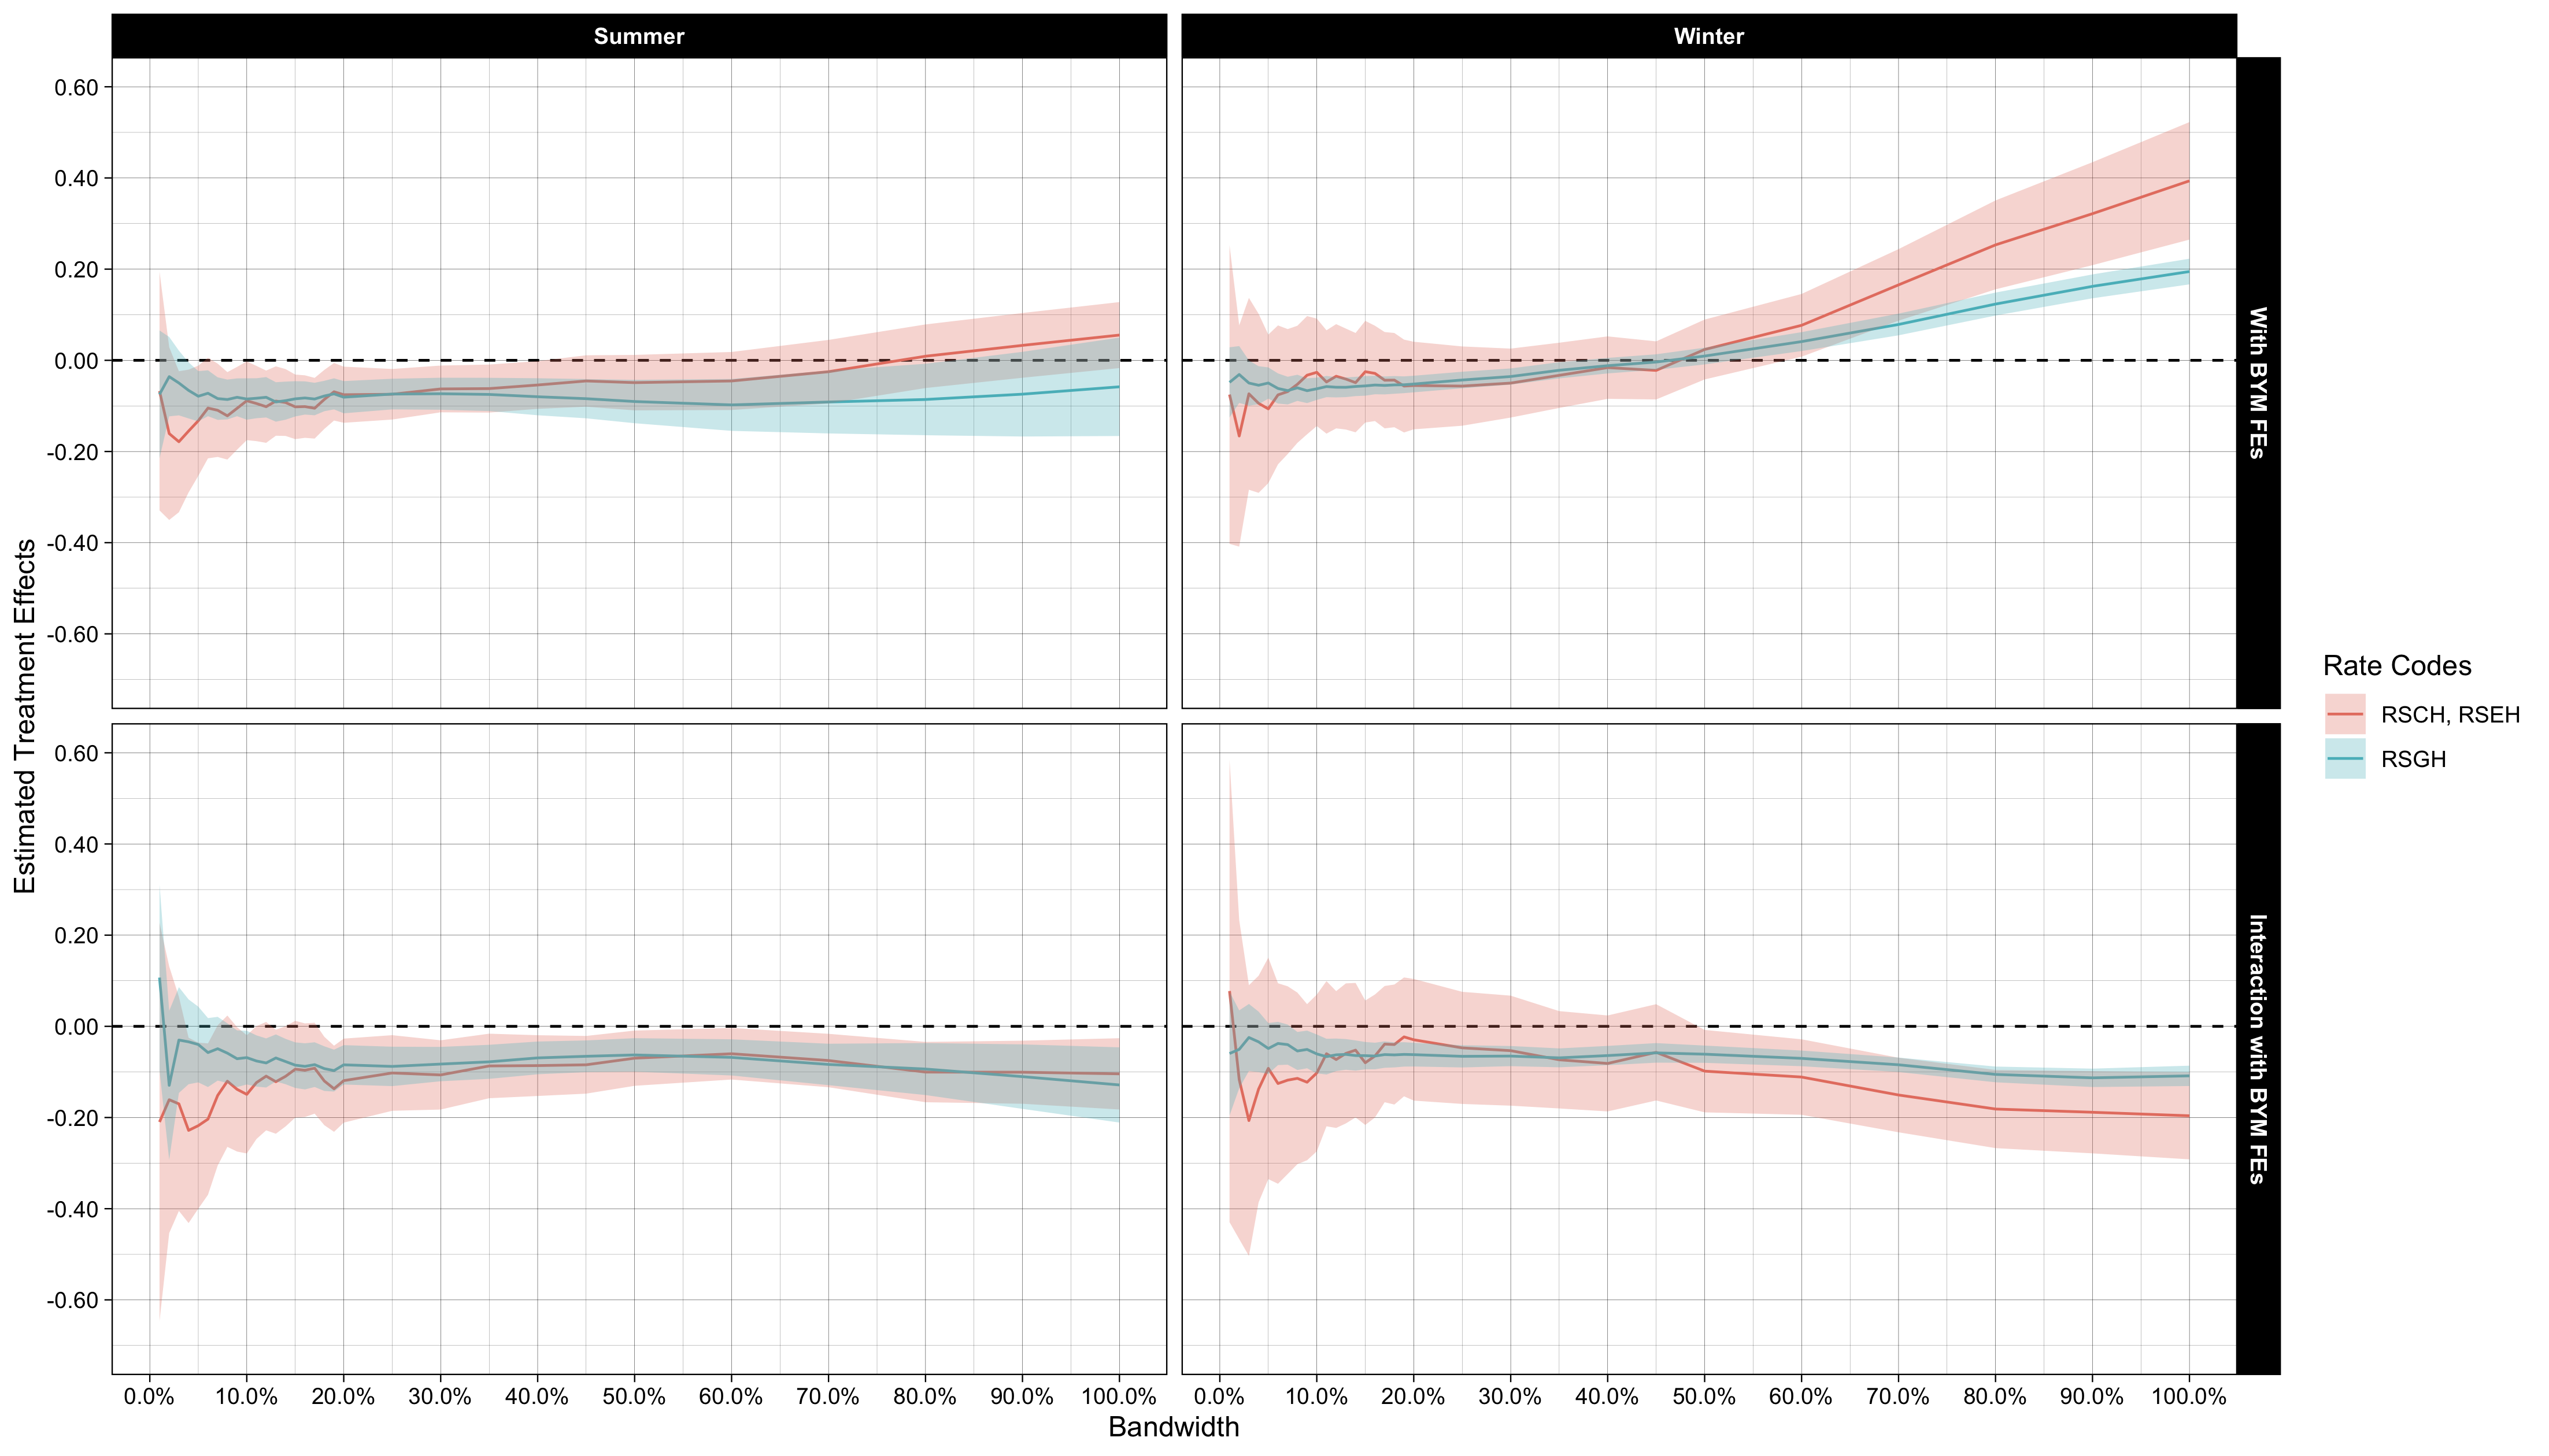
\includegraphics[scale = 0.108]{02_Plots/Regression-Results_RD-Design_Treatment-Effect-by-BW-and-Rate-Codes_Square}
        \caption{Models with Square Term of Running Variable}
        \label{Figure:Estimated-Treatment-Effects_By-Rate-Code-and-Season_Square}
    \end{subfigure}
    \newline
    \begin{subfigure}{1.0\textwidth}
        \centering
        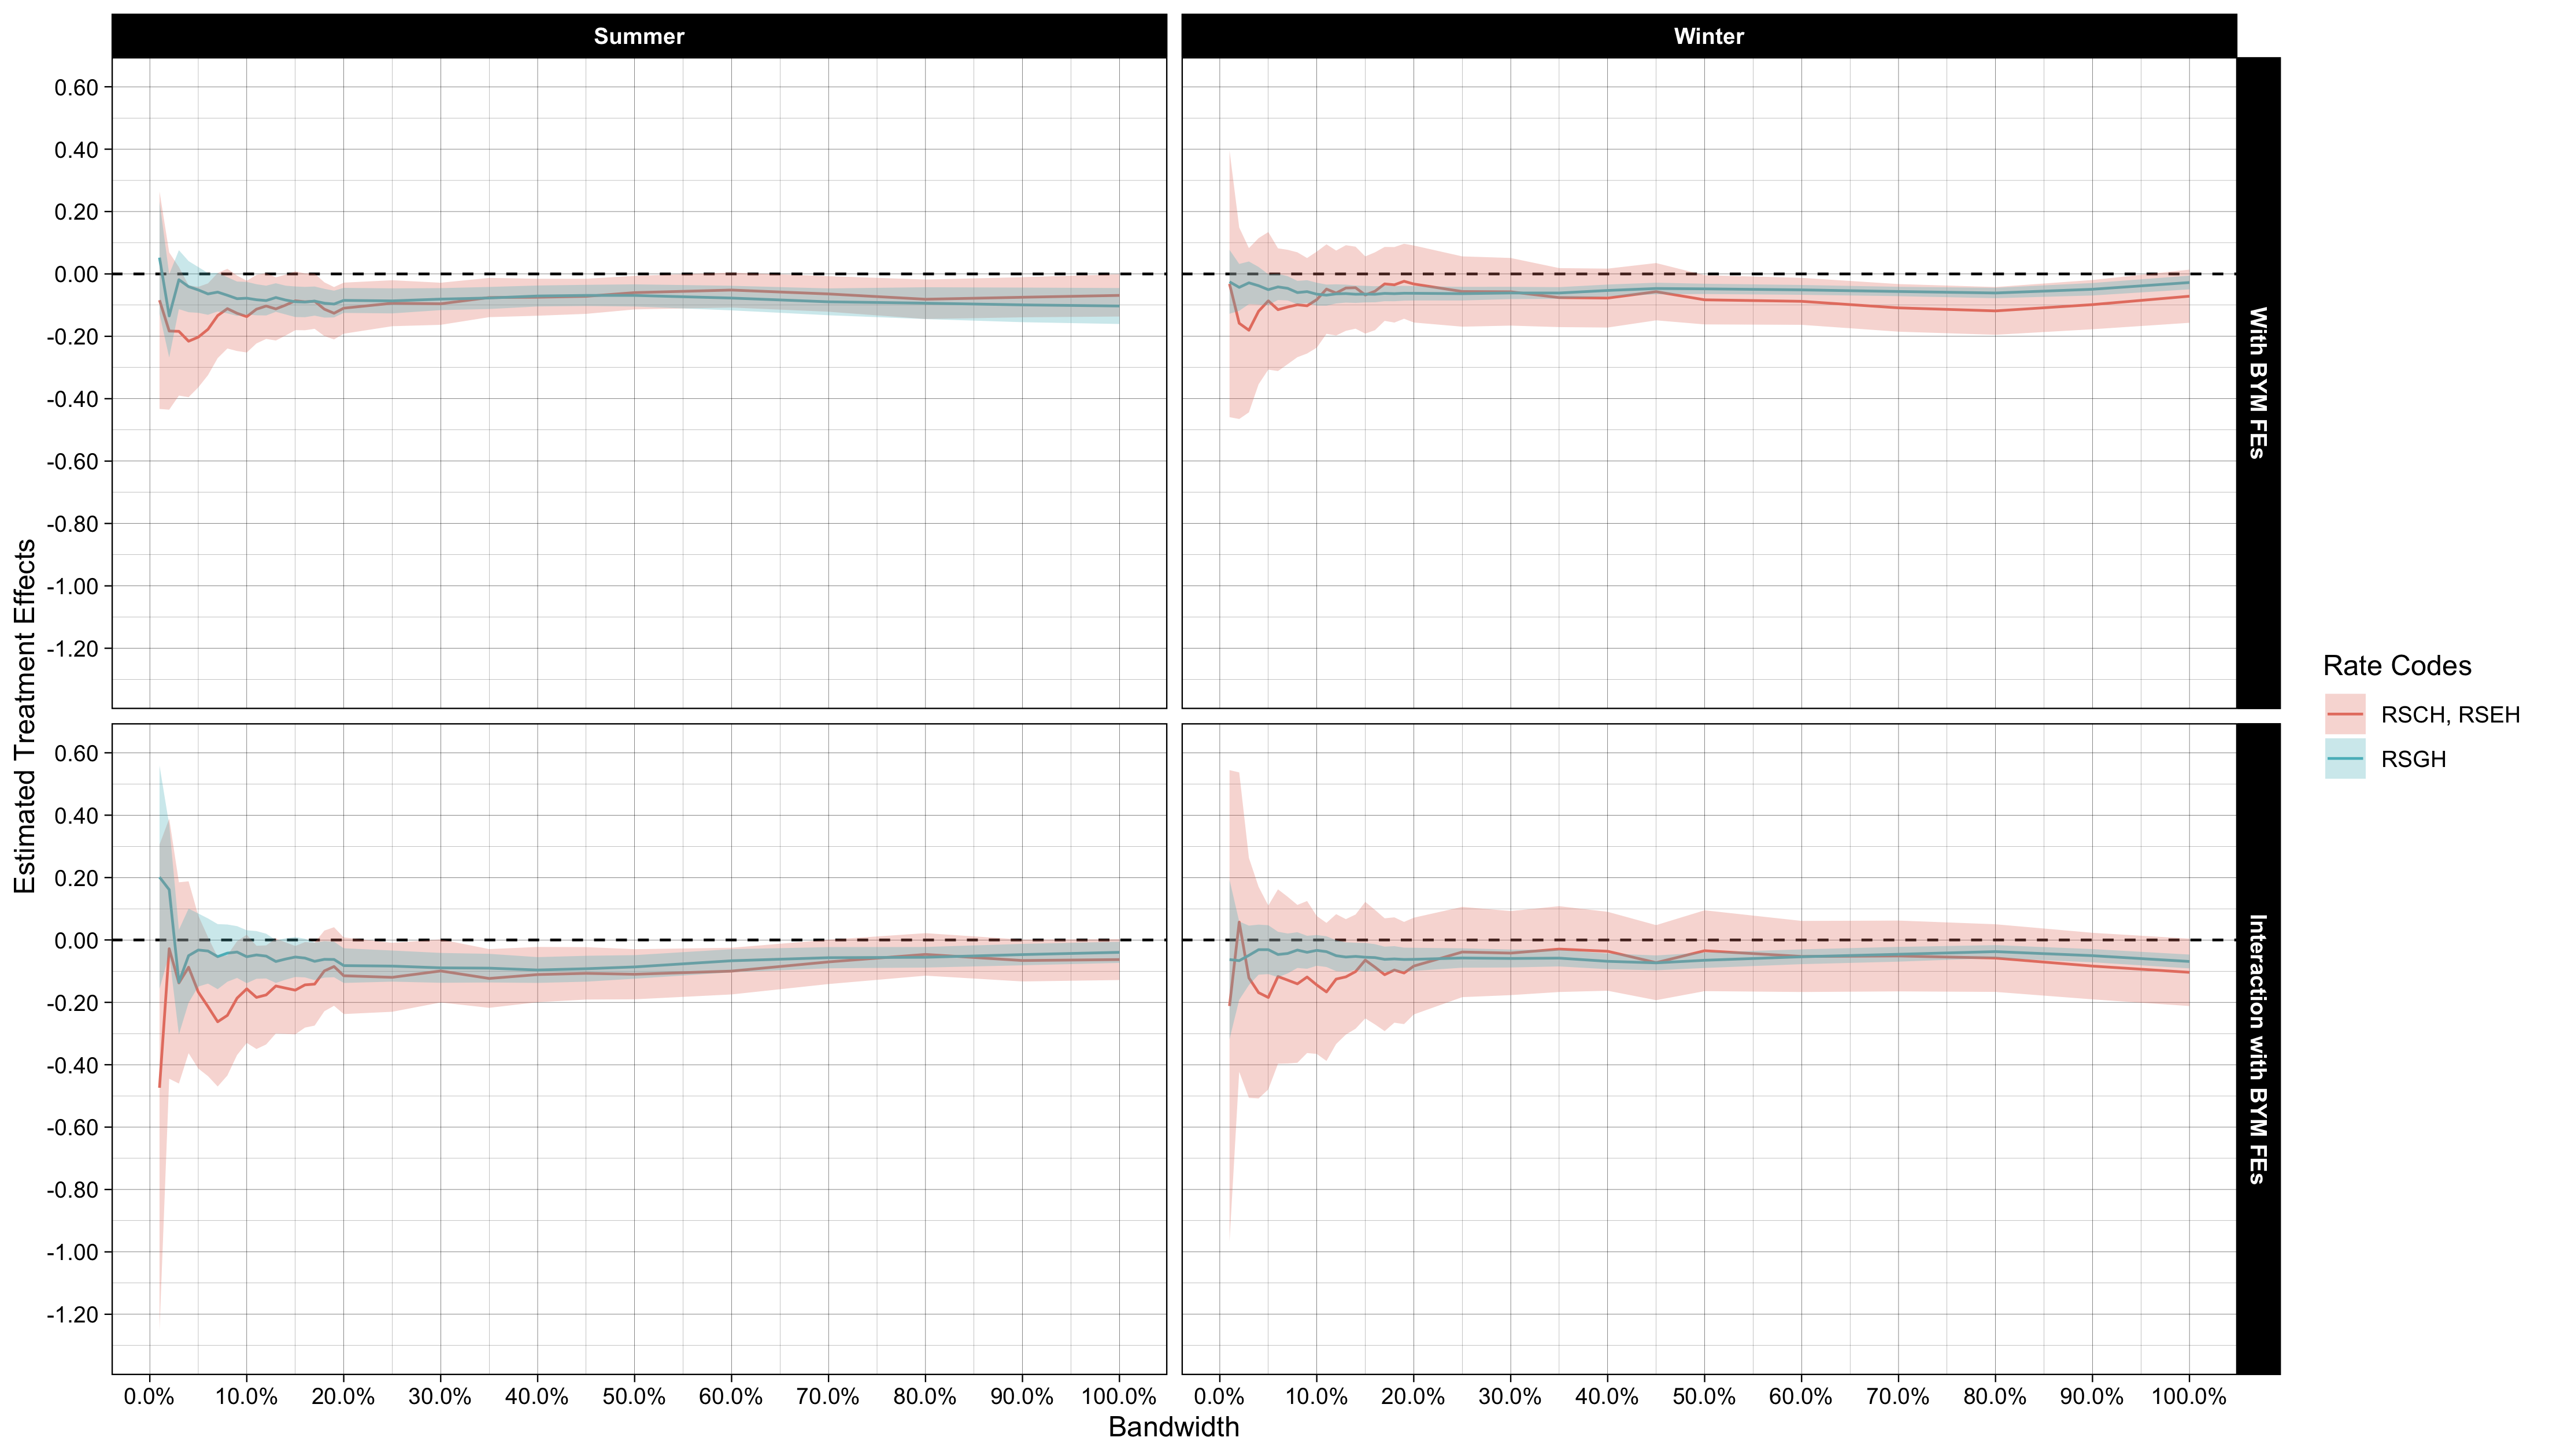
\includegraphics[scale = 0.108]{02_Plots/Regression-Results_RD-Design_Treatment-Effect-by-BW-and-Rate-Codes_Cubic}
        \caption{Models with Cubic Term of Running Variable}
        \label{Figure:Estimated-Treatment-Effects_By-Rate-Code-and-Season_Cubic}
    \end{subfigure}
    \caption{Estimated Treatment Effects by Bandwidth, Rate Code, and Season}
    \subcaption*{\textit{Notes}: Standard errors are selected between heteroskedasticity-robust and clustered (by Account-Premise IDs and Billing Year-Month) standard errors. Shaded areas in each panel indicate the 95\% confidence intervals. RSCH and RSEH rate codes have the same base usage qty, as illustrated in Figure \ref{Figure:Residential-Rate-Schedules_Base-Usage-Qty_By-Rate-Code}. When estimating the treatment effect, observations satisfying following conditions are exploited only: 1) observations between 2005 and 2011, and 2) observations without in-period seasonal change in Base Usage Qty.}
\end{figure}

\clearpage
%\begin{figure}
%    \begin{subfigure}{1.0\textwidth}
%        \centering
%        \includegraphics[scale = 0.143]{02_Plots/Regression-Results_RD-Design_Treatment-Effect-by-Term-between-Periods_RSCH-RSEH}
%        \caption{RSCH \& RSEH}
%        \vspace{0.1cm}
%    \end{subfigure}
%    \newline
%    \begin{subfigure}{1.0\textwidth}
%        \centering
%        \includegraphics[scale = 0.143]{02_Plots/Regression-Results_RD-Design_Treatment-Effect-by-Term-between-Periods_RSGH}
%        \caption{RSGH}
%    \end{subfigure}
%    \caption{Estimated Treatment Effects by Bandwidth and Term(s) between Periods}
%    \label{Figure:Estimated-Treatment-Effects_By-Terms-between-Periods}
%    \subcaption*{\textit{Notes}: Only for five bandwidths, the treatment effects are estimated. The term(s) between periods has the value of 1 (2, 3, and so on) when period 0 and period 1 (period 0 and period 2, period 0 and period 3, and so on) data are used to estimate the treatment effects. Standard errors are selected between heteroskedasticity-robust and clustered (by Account-Premise IDs and Billing Year-Month) standard errors. Error bars indicate the 95\% confidence intervals. Both point estimates and error bars are jittered for readability. RSCH and RSEH rate codes have the same base usage qty, as illustrated in Figure \ref{Figure:Residential-Rate-Schedules_Base-Usage-Qty_By-Rate-Code}. When estimating the treatment effect, observations satisfying following conditions are exploited only: 1) observations between 2005 and 2011, and 2) observations without in-period seasonal change in Base Usage Qty.}
%\end{figure}


\clearpage
\subsection{Miscellaneous Plots}
\vspace{0.5cm}

\begin{figure}
    \centering
    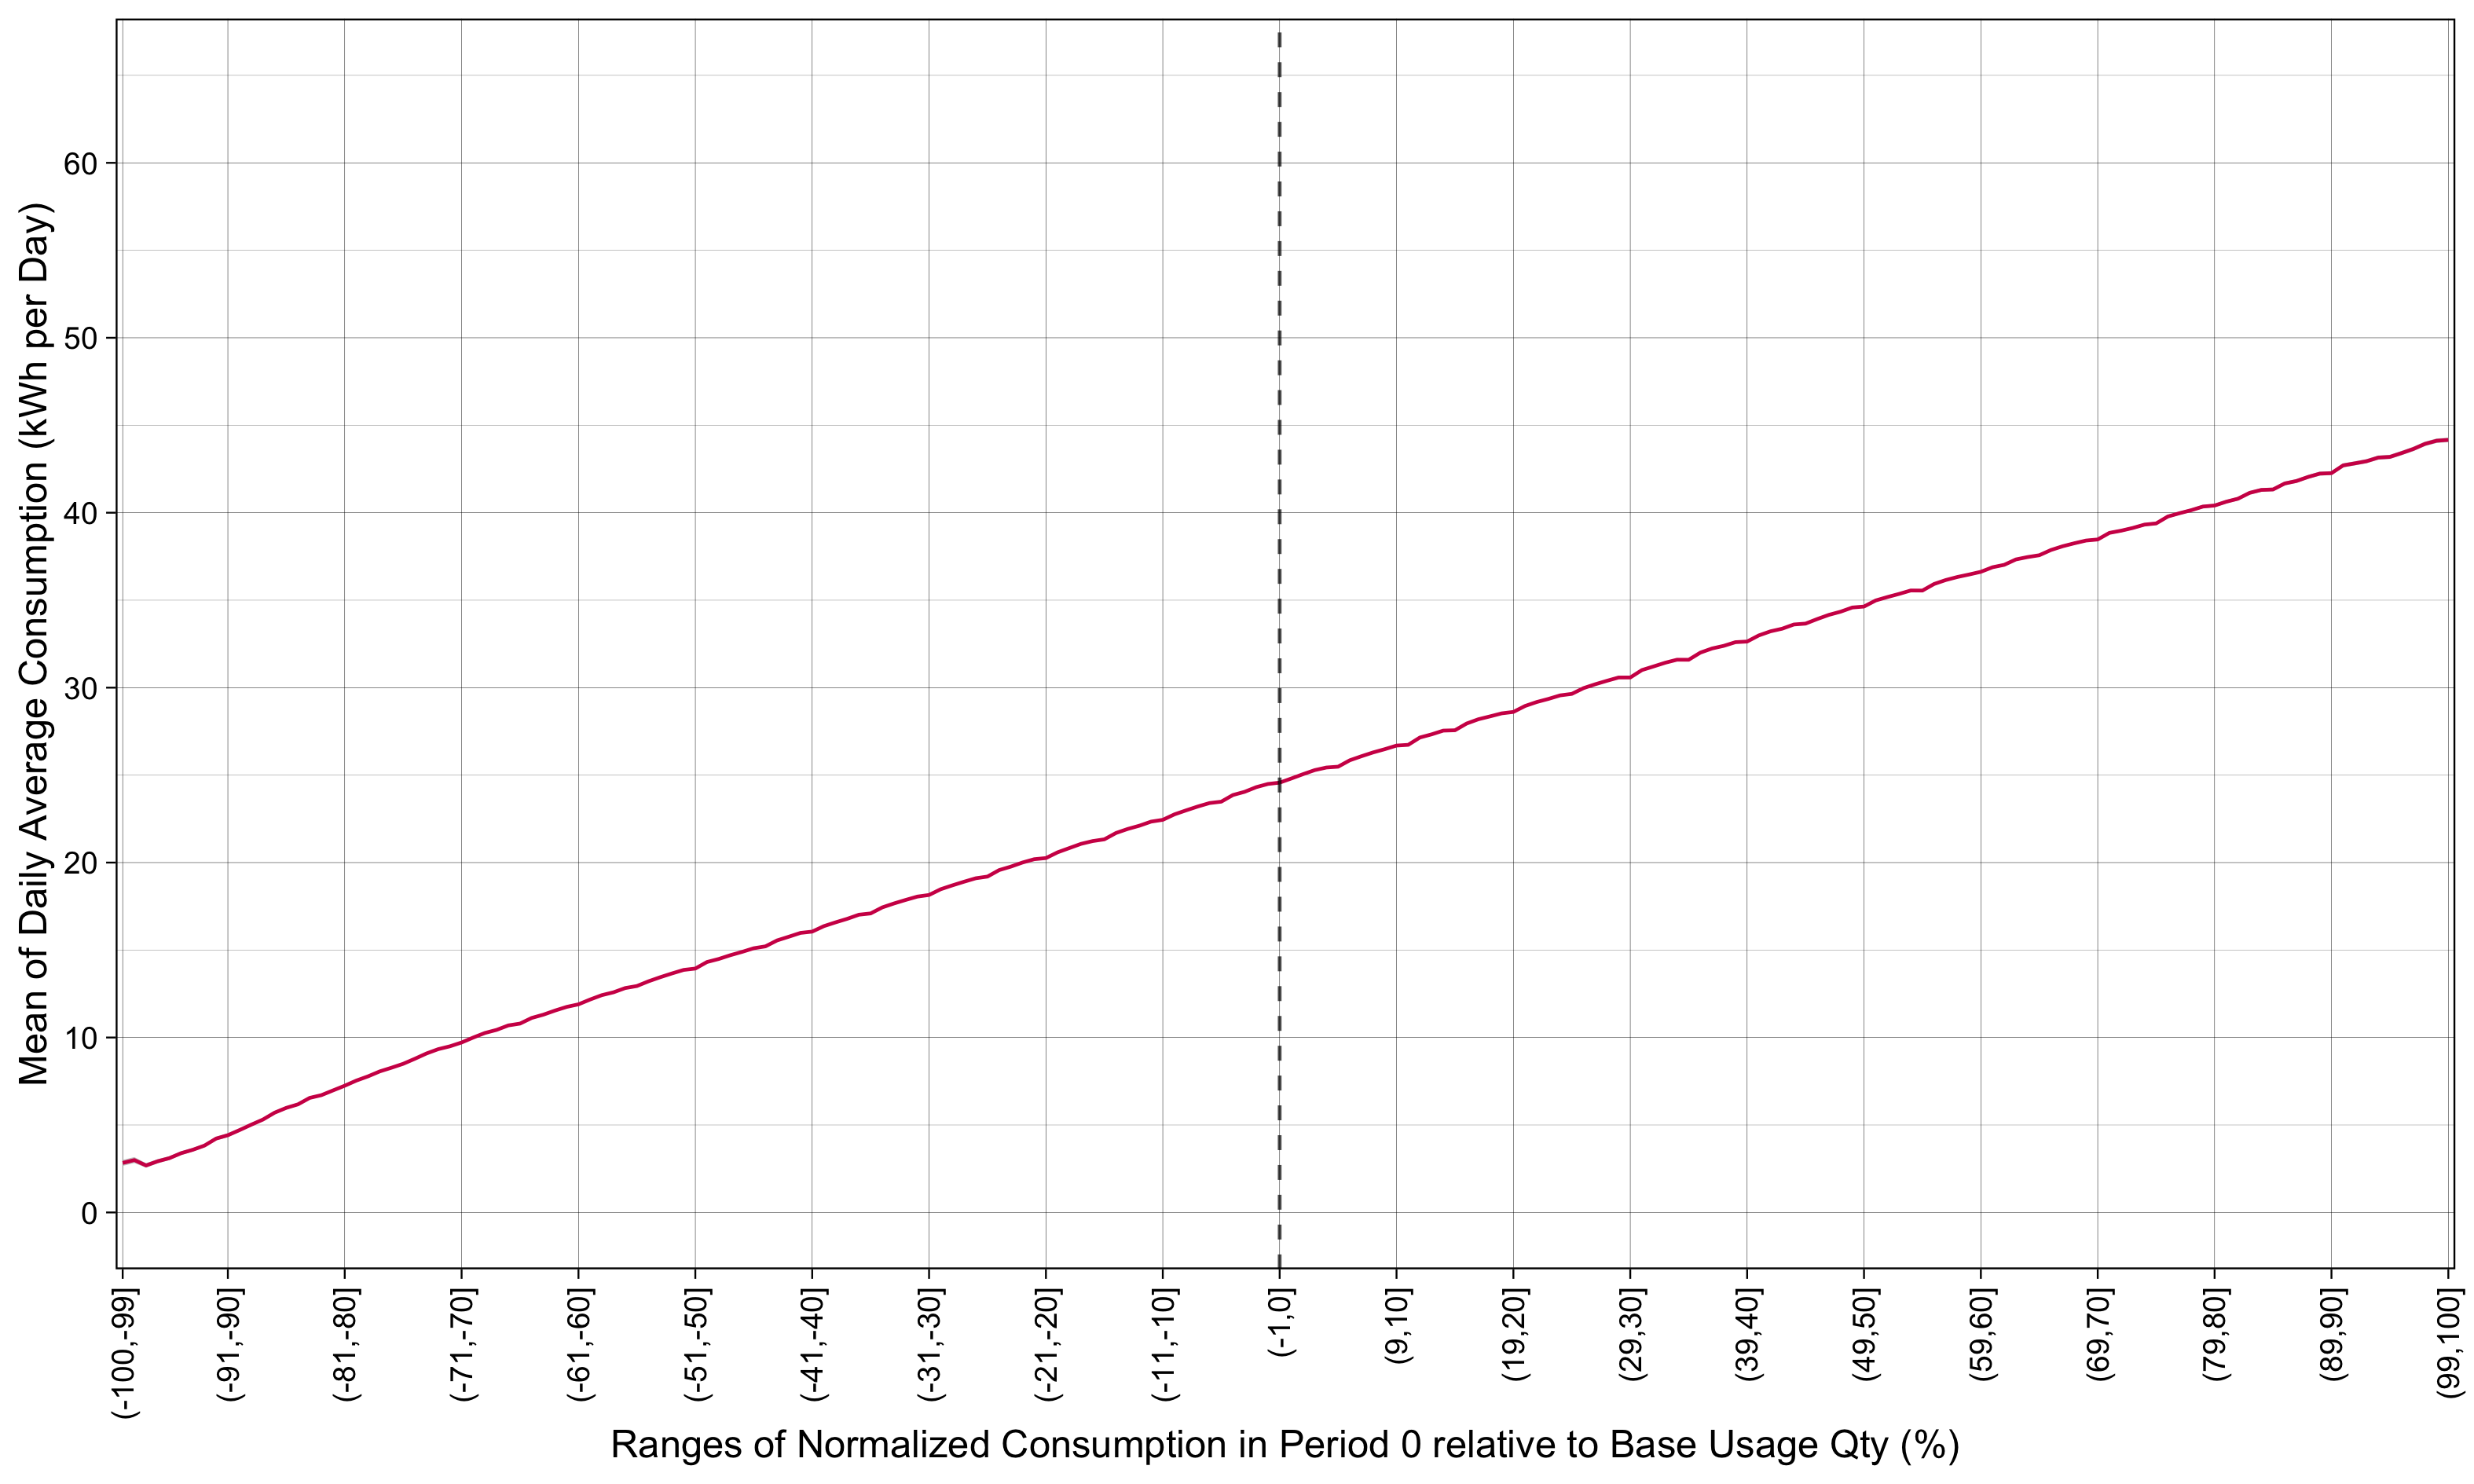
\includegraphics[scale = 0.15]{02_Plots/SMUD-Billing-Data_RD-Design_Mean-by-Range}
    \caption{Mean of Daily Average Consumption by Range of Normalized Consumption in Period 0 (\%)}
    \subcaption*{\textit{Notes}: Un-restricted sample is used to create this figure. Grey area indicates the 95\% confidence interval.}
    \label{Figure:Mean-by-Ranges}
\end{figure}




% ------- Back-Matter -------
%\backmatter


\end{document}

